% Options for packages loaded elsewhere
\PassOptionsToPackage{unicode}{hyperref}
\PassOptionsToPackage{hyphens}{url}
%
\documentclass[
  oneside,
  openany]{book}
\usepackage{amsmath,amssymb}
\usepackage{iftex}
\ifPDFTeX
  \usepackage[T1]{fontenc}
  \usepackage[utf8]{inputenc}
  \usepackage{textcomp} % provide euro and other symbols
\else % if luatex or xetex
  \usepackage{unicode-math} % this also loads fontspec
  \defaultfontfeatures{Scale=MatchLowercase}
  \defaultfontfeatures[\rmfamily]{Ligatures=TeX,Scale=1}
\fi
\usepackage{lmodern}
\ifPDFTeX\else
  % xetex/luatex font selection
\fi
% Use upquote if available, for straight quotes in verbatim environments
\IfFileExists{upquote.sty}{\usepackage{upquote}}{}
\IfFileExists{microtype.sty}{% use microtype if available
  \usepackage[]{microtype}
  \UseMicrotypeSet[protrusion]{basicmath} % disable protrusion for tt fonts
}{}
\makeatletter
\@ifundefined{KOMAClassName}{% if non-KOMA class
  \IfFileExists{parskip.sty}{%
    \usepackage{parskip}
  }{% else
    \setlength{\parindent}{0pt}
    \setlength{\parskip}{6pt plus 2pt minus 1pt}}
}{% if KOMA class
  \KOMAoptions{parskip=half}}
\makeatother
\usepackage{xcolor}
\usepackage[margin=1in]{geometry}
\usepackage{color}
\usepackage{fancyvrb}
\newcommand{\VerbBar}{|}
\newcommand{\VERB}{\Verb[commandchars=\\\{\}]}
\DefineVerbatimEnvironment{Highlighting}{Verbatim}{commandchars=\\\{\}}
% Add ',fontsize=\small' for more characters per line
\usepackage{framed}
\definecolor{shadecolor}{RGB}{248,248,248}
\newenvironment{Shaded}{\begin{snugshade}}{\end{snugshade}}
\newcommand{\AlertTok}[1]{\textcolor[rgb]{0.94,0.16,0.16}{#1}}
\newcommand{\AnnotationTok}[1]{\textcolor[rgb]{0.56,0.35,0.01}{\textbf{\textit{#1}}}}
\newcommand{\AttributeTok}[1]{\textcolor[rgb]{0.13,0.29,0.53}{#1}}
\newcommand{\BaseNTok}[1]{\textcolor[rgb]{0.00,0.00,0.81}{#1}}
\newcommand{\BuiltInTok}[1]{#1}
\newcommand{\CharTok}[1]{\textcolor[rgb]{0.31,0.60,0.02}{#1}}
\newcommand{\CommentTok}[1]{\textcolor[rgb]{0.56,0.35,0.01}{\textit{#1}}}
\newcommand{\CommentVarTok}[1]{\textcolor[rgb]{0.56,0.35,0.01}{\textbf{\textit{#1}}}}
\newcommand{\ConstantTok}[1]{\textcolor[rgb]{0.56,0.35,0.01}{#1}}
\newcommand{\ControlFlowTok}[1]{\textcolor[rgb]{0.13,0.29,0.53}{\textbf{#1}}}
\newcommand{\DataTypeTok}[1]{\textcolor[rgb]{0.13,0.29,0.53}{#1}}
\newcommand{\DecValTok}[1]{\textcolor[rgb]{0.00,0.00,0.81}{#1}}
\newcommand{\DocumentationTok}[1]{\textcolor[rgb]{0.56,0.35,0.01}{\textbf{\textit{#1}}}}
\newcommand{\ErrorTok}[1]{\textcolor[rgb]{0.64,0.00,0.00}{\textbf{#1}}}
\newcommand{\ExtensionTok}[1]{#1}
\newcommand{\FloatTok}[1]{\textcolor[rgb]{0.00,0.00,0.81}{#1}}
\newcommand{\FunctionTok}[1]{\textcolor[rgb]{0.13,0.29,0.53}{\textbf{#1}}}
\newcommand{\ImportTok}[1]{#1}
\newcommand{\InformationTok}[1]{\textcolor[rgb]{0.56,0.35,0.01}{\textbf{\textit{#1}}}}
\newcommand{\KeywordTok}[1]{\textcolor[rgb]{0.13,0.29,0.53}{\textbf{#1}}}
\newcommand{\NormalTok}[1]{#1}
\newcommand{\OperatorTok}[1]{\textcolor[rgb]{0.81,0.36,0.00}{\textbf{#1}}}
\newcommand{\OtherTok}[1]{\textcolor[rgb]{0.56,0.35,0.01}{#1}}
\newcommand{\PreprocessorTok}[1]{\textcolor[rgb]{0.56,0.35,0.01}{\textit{#1}}}
\newcommand{\RegionMarkerTok}[1]{#1}
\newcommand{\SpecialCharTok}[1]{\textcolor[rgb]{0.81,0.36,0.00}{\textbf{#1}}}
\newcommand{\SpecialStringTok}[1]{\textcolor[rgb]{0.31,0.60,0.02}{#1}}
\newcommand{\StringTok}[1]{\textcolor[rgb]{0.31,0.60,0.02}{#1}}
\newcommand{\VariableTok}[1]{\textcolor[rgb]{0.00,0.00,0.00}{#1}}
\newcommand{\VerbatimStringTok}[1]{\textcolor[rgb]{0.31,0.60,0.02}{#1}}
\newcommand{\WarningTok}[1]{\textcolor[rgb]{0.56,0.35,0.01}{\textbf{\textit{#1}}}}
\usepackage{longtable,booktabs,array}
\usepackage{calc} % for calculating minipage widths
% Correct order of tables after \paragraph or \subparagraph
\usepackage{etoolbox}
\makeatletter
\patchcmd\longtable{\par}{\if@noskipsec\mbox{}\fi\par}{}{}
\makeatother
% Allow footnotes in longtable head/foot
\IfFileExists{footnotehyper.sty}{\usepackage{footnotehyper}}{\usepackage{footnote}}
\makesavenoteenv{longtable}
\usepackage{graphicx}
\makeatletter
\def\maxwidth{\ifdim\Gin@nat@width>\linewidth\linewidth\else\Gin@nat@width\fi}
\def\maxheight{\ifdim\Gin@nat@height>\textheight\textheight\else\Gin@nat@height\fi}
\makeatother
% Scale images if necessary, so that they will not overflow the page
% margins by default, and it is still possible to overwrite the defaults
% using explicit options in \includegraphics[width, height, ...]{}
\setkeys{Gin}{width=\maxwidth,height=\maxheight,keepaspectratio}
% Set default figure placement to htbp
\makeatletter
\def\fps@figure{htbp}
\makeatother
\usepackage{svg}
\setlength{\emergencystretch}{3em} % prevent overfull lines
\providecommand{\tightlist}{%
  \setlength{\itemsep}{0pt}\setlength{\parskip}{0pt}}
\setcounter{secnumdepth}{5}
\usepackage{booktabs}
\usepackage{longtable}
\ifLuaTeX
  \usepackage{selnolig}  % disable illegal ligatures
\fi
\usepackage{bookmark}
\IfFileExists{xurl.sty}{\usepackage{xurl}}{} % add URL line breaks if available
\urlstyle{same}
\hypersetup{
  pdftitle={lifesimulatoR Book},
  pdfauthor={Noushin Nabavi},
  hidelinks,
  pdfcreator={LaTeX via pandoc}}

\title{lifesimulatoR Book}
\author{Noushin Nabavi}
\date{2026-06-20}

\begin{document}
\maketitle

{
\setcounter{tocdepth}{1}
\tableofcontents
}
\href{https://doi.org/10.5281/zenodo.20767188}{\includesvg{lifesimulatoR-book_files/55082e2caad9809d8098b0283082b306832db062.svg}}

\chapter*{Welcome}\label{welcome}
\addcontentsline{toc}{chapter}{Welcome}

The origin of life is one of the deepest and most challenging questions in science. It asks how non-living matter became organized enough to exhibit the properties we associate with living systems, including replication, variation, heredity, metabolism, adaptation, and evolution.

Unlike many scientific questions, the origin of life sits at the intersection of multiple disciplines. Chemistry seeks to understand how biological building blocks could form naturally. Biology examines how information and evolution emerged. Physics explores energy flow and self-organization. Geology provides clues about the environments of the early Earth. Complexity science investigates how interacting systems can generate emergent behavior.

At its core, the origin-of-life problem can be summarized by a simple question:

\begin{quote}
How can chemistry become biology?
\end{quote}

Despite decades of research, there is currently no universally accepted explanation. Instead, several major scientific frameworks have been proposed.

The \textbf{RNA World} hypothesis suggests that life may have begun with RNA-like molecules capable of both storing information and catalyzing reactions. \textbf{Metabolism-First} theories propose that self-sustaining reaction networks emerged before genetic systems. \textbf{Protocell} theories emphasize the importance of compartments and primitive membranes. \textbf{Autocatalytic Set Theory} focuses on networks of molecules that collectively support their own production. Increasingly, researchers view these theories as complementary rather than competing, suggesting that life may have emerged through interactions among molecules, networks, compartments, and environmental energy sources.

Although these theories differ in emphasis, most agree that life-like systems require several key ingredients:

\begin{enumerate}
\def\labelenumi{\arabic{enumi}.}
\tightlist
\item
  Variation
\item
  Persistence
\item
  Replication or reproduction
\item
  Mutation and novelty
\item
  Selection
\item
  Organization
\item
  Compartmentalization
\item
  Energy flow
\end{enumerate}

Understanding how these ingredients became linked remains one of the central challenges of modern science.

This book serves as the theoretical companion to the \texttt{lifesimulatoR} package. The package provides simplified computational simulations that allow readers to explore many of the ideas discussed in origin-of-life research. Rather than attempting to reproduce the full complexity of early Earth chemistry, the simulations focus on fundamental concepts such as mutation, selection, diversity, autocatalysis, compartmentalization, and emergence.

The goal is not to demonstrate how life actually originated. Instead, the goal is to provide conceptual tools that help illuminate the logic underlying major origin-of-life theories.

\section*{What is lifesimulatoR?}\label{what-is-lifesimulator}
\addcontentsline{toc}{section}{What is lifesimulatoR?}

\texttt{lifesimulatoR} is an educational R package designed to explore simplified models of abiogenesis and early evolution.

The package includes tools for:

\begin{itemize}
\tightlist
\item
  Creating symbolic molecular populations
\item
  Simulating mutation and replication
\item
  Exploring evolutionary dynamics
\item
  Measuring diversity and entropy
\item
  Modeling protocell populations
\item
  Simulating autocatalytic networks
\item
  Visualizing simulation outputs
\end{itemize}

These models are intentionally simplified so that the underlying concepts remain accessible and transparent.

\section*{How this book is organized}\label{how-this-book-is-organized}
\addcontentsline{toc}{section}{How this book is organized}

The book follows a progression from chemistry toward increasingly life-like systems.

\textbf{Origin of Life: Big Questions} introduces the scientific problem and the major theories that attempt to explain life's emergence.

\textbf{Prebiotic Chemistry and Molecular Pools} examines how molecular diversity may have arisen on the early Earth.

\textbf{Molecular Evolution} explores how replication, mutation, heredity, and selection can produce evolutionary change.

\textbf{Diversity, Entropy, and Complexity} investigates how variation can be quantified and how complexity differs from randomness.

\textbf{Protocells and Compartmentalization} examines how boundaries may have helped organize early chemistry.

\textbf{Autocatalytic Networks} explores how networks of interacting molecules can become self-reinforcing and self-maintaining.

\textbf{Comparing Origin-of-Life Frameworks} integrates the major theories and discusses open questions and future research directions.

The appendices provide function references, classroom activities, and additional resources for educators and students.

\section*{How to use this book}\label{how-to-use-this-book}
\addcontentsline{toc}{section}{How to use this book}

This book can be approached in several ways.

Students may use it as a self-study introduction to origin-of-life science.

Instructors may use it as a teaching companion for courses in biology, chemistry, complexity science, astrobiology, or systems thinking.

Researchers and science communicators may use it as a conceptual framework for discussing major ideas in abiogenesis.

Readers are encouraged to modify examples, experiment with parameter values, compare simulation outcomes, and critically evaluate model assumptions.

\section*{A Simple Example}\label{a-simple-example}
\addcontentsline{toc}{section}{A Simple Example}

The package can be used to simulate a simplified evolutionary process.

\begin{Shaded}
\begin{Highlighting}[]
\NormalTok{sim }\OtherTok{\textless{}{-}} \FunctionTok{simulate\_abiogenesis}\NormalTok{(}
  \AttributeTok{n\_molecules =} \DecValTok{100}\NormalTok{,}
  \AttributeTok{generations =} \DecValTok{100}\NormalTok{,}
  \AttributeTok{mutation\_rate =} \FloatTok{0.02}\NormalTok{,}
  \AttributeTok{selection\_strength =} \DecValTok{1}\NormalTok{,}
  \AttributeTok{seed =} \DecValTok{123}
\NormalTok{)}

\FunctionTok{head}\NormalTok{(sim)}
\end{Highlighting}
\end{Shaded}

\begin{verbatim}
## # A tibble: 6 x 6
##   generation n_molecules mean_length mean_fitness diversity max_fitness
##        <int>       <int>       <dbl>        <dbl>     <int>       <dbl>
## 1          0         100        12.6         1.00       100        1.25
## 2          1         100        12.7         1.04        67        1.25
## 3          2         100        12.3         1.05        61        1.25
## 4          3         100        12.3         1.11        61        1.25
## 5          4         100        12.5         1.11        48        1.25
## 6          5         100        12.8         1.13        53        1.25
\end{verbatim}

Simulation outputs can be visualized using:

\begin{Shaded}
\begin{Highlighting}[]
\FunctionTok{plot\_simulation}\NormalTok{(}
\NormalTok{  sim,}
  \AttributeTok{x =} \StringTok{"generation"}\NormalTok{,}
  \AttributeTok{y =} \StringTok{"mean\_fitness"}
\NormalTok{)}
\end{Highlighting}
\end{Shaded}

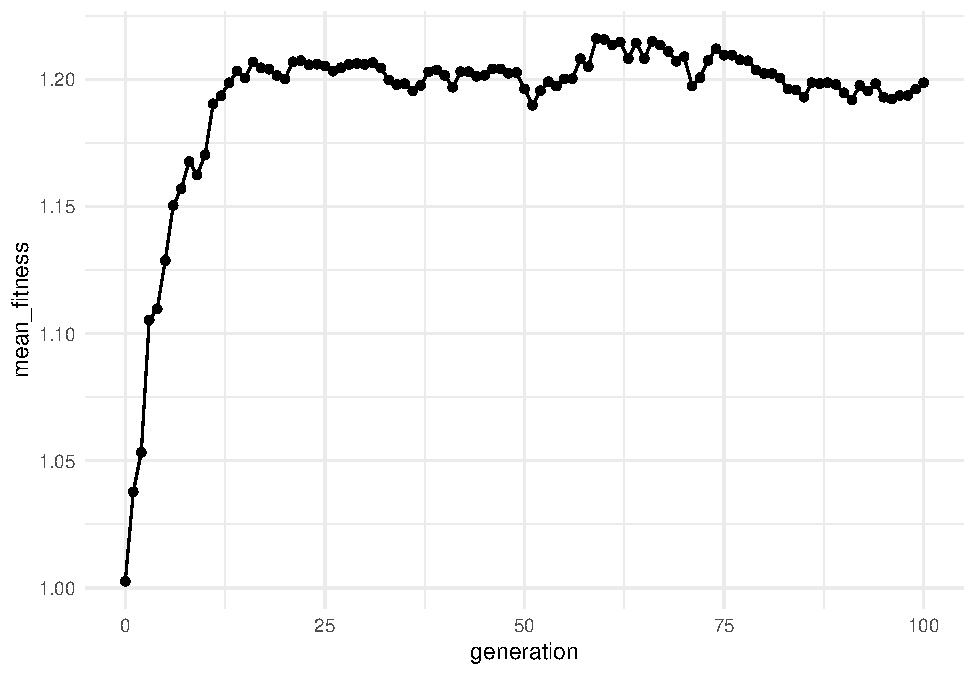
\includegraphics{lifesimulatoR-book_files/lifesimulatoR-book_files/figure-latex/welcome-plot-1.pdf}

These simulations do not represent the actual origin of life. Instead, they illustrate how variation, mutation, replication, and selection can produce population-level change through time.

\section*{Important Interpretation Note}\label{important-interpretation-note}
\addcontentsline{toc}{section}{Important Interpretation Note}

The simulations in \texttt{lifesimulatoR} are educational models.

They do not include realistic chemistry, thermodynamics, environmental variability, molecular folding, or detailed reaction kinetics. Consequently, simulation results should not be interpreted as evidence supporting a specific origin-of-life theory.

Instead, the models are best viewed as conceptual laboratories that allow readers to explore ideas, test assumptions, and develop intuition about the mechanisms frequently discussed in origin-of-life research.

\section*{Moving Forward}\label{moving-forward}
\addcontentsline{toc}{section}{Moving Forward}

The chapters that follow examine the major scientific ideas behind life's emergence, beginning with the fundamental question of how non-living chemistry could generate the diversity and organization required for evolution to begin.

\chapter{Origin of Life: Big Questions}\label{origin-of-life-big-questions}

\section{Why this question matters}\label{why-this-question-matters}

The origin of life is one of the most important open questions in science. It asks how non-living matter could give rise to systems that show life-like properties such as persistence, replication, variation, heredity, metabolism, and evolution.

This question sits at the intersection of chemistry, biology, geology, physics, information theory, and complexity science. It is not only about identifying the first living organism. It is also about understanding how matter became organized enough to evolve.

A useful way to frame the problem is:

\begin{quote}
How can chemistry become biology?
\end{quote}

\section{Major origin-of-life theories}\label{major-origin-of-life-theories}

There is no single universally accepted theory of the origin of life. Instead, there are several major research traditions.

\begin{longtable}[]{@{}
  >{\raggedright\arraybackslash}p{(\columnwidth - 4\tabcolsep) * \real{0.1319}}
  >{\raggedright\arraybackslash}p{(\columnwidth - 4\tabcolsep) * \real{0.5000}}
  >{\raggedright\arraybackslash}p{(\columnwidth - 4\tabcolsep) * \real{0.3681}}@{}}
\toprule\noalign{}
\begin{minipage}[b]{\linewidth}\raggedright
Theory
\end{minipage} & \begin{minipage}[b]{\linewidth}\raggedright
Main idea
\end{minipage} & \begin{minipage}[b]{\linewidth}\raggedright
Central challenge
\end{minipage} \\
\midrule\noalign{}
\endhead
\bottomrule\noalign{}
\endlastfoot
RNA World & Life began with RNA-like molecules capable of storing information and catalyzing reactions. & How did RNA-like molecules form and replicate reliably? \\
Metabolism First & Self-sustaining reaction networks emerged before genetic replication. & How did such networks become stable and evolvable? \\
Protocell First & Compartments played a central role in organizing chemistry. & How did compartments grow, divide, and preserve internal chemistry? \\
Autocatalytic Set Theory & Networks of mutually reinforcing molecules produced self-maintaining systems. & How did network organization become heritable? \\
Hybrid Models & Life emerged through coupling among molecules, compartments, energy flows, and networks. & How did these processes become integrated? \\
\end{longtable}

These theories are not always mutually exclusive. A complete account may need to explain how molecular information, metabolism, compartments, and energy flow became linked.

\section{Conceptual model}\label{conceptual-model}

A minimal life-like system may need several ingredients:

\begin{enumerate}
\def\labelenumi{\arabic{enumi}.}
\tightlist
\item
  \textbf{Variation}: molecules or systems must differ.
\item
  \textbf{Persistence}: some variants must last longer than others.
\item
  \textbf{Replication or reproduction}: successful variants must influence future states.
\item
  \textbf{Mutation or novelty}: new variants must appear.
\item
  \textbf{Selection}: some variants must become more common.
\item
  \textbf{Organization}: components must interact in structured ways.
\end{enumerate}

In \texttt{lifesimulatoR}, these ideas are represented using symbolic molecules and simple simulations. The package does not attempt to reproduce real prebiotic chemistry. Instead, it provides simplified computational models for exploring the logic of origin-of-life ideas.

\section{Package example: a simple molecular evolution simulation}\label{package-example-a-simple-molecular-evolution-simulation}

The following simulation begins with a symbolic molecular population. Over repeated generations, molecules are copied, mutated, and selected according to a simplified fitness rule.

\begin{Shaded}
\begin{Highlighting}[]
\NormalTok{sim }\OtherTok{\textless{}{-}} \FunctionTok{simulate\_abiogenesis}\NormalTok{(}
  \AttributeTok{n\_molecules =} \DecValTok{100}\NormalTok{,}
  \AttributeTok{generations =} \DecValTok{100}\NormalTok{,}
  \AttributeTok{mutation\_rate =} \FloatTok{0.02}\NormalTok{,}
  \AttributeTok{selection\_strength =} \DecValTok{1}\NormalTok{,}
  \AttributeTok{seed =} \DecValTok{123}
\NormalTok{)}

\FunctionTok{head}\NormalTok{(sim)}
\end{Highlighting}
\end{Shaded}

\begin{verbatim}
## # A tibble: 6 x 6
##   generation n_molecules mean_length mean_fitness diversity max_fitness
##        <int>       <int>       <dbl>        <dbl>     <int>       <dbl>
## 1          0         100        12.6         1.00       100        1.25
## 2          1         100        12.7         1.04        67        1.25
## 3          2         100        12.3         1.05        61        1.25
## 4          3         100        12.3         1.11        61        1.25
## 5          4         100        12.5         1.11        48        1.25
## 6          5         100        12.8         1.13        53        1.25
\end{verbatim}

The output is a time series. Each row summarizes the state of the molecular population at a generation.

Depending on the package version, the output may include variables such as:

\begin{itemize}
\tightlist
\item
  generation number,
\item
  number of molecules,
\item
  mean fitness,
\item
  maximum fitness,
\item
  diversity,
\item
  mean sequence length.
\end{itemize}

\section{Visualizing change through time}\label{visualizing-change-through-time}

\begin{Shaded}
\begin{Highlighting}[]
\FunctionTok{plot\_simulation}\NormalTok{(}
\NormalTok{  sim,}
  \AttributeTok{x =} \StringTok{"generation"}\NormalTok{,}
  \AttributeTok{y =} \StringTok{"mean\_fitness"}
\NormalTok{)}
\end{Highlighting}
\end{Shaded}

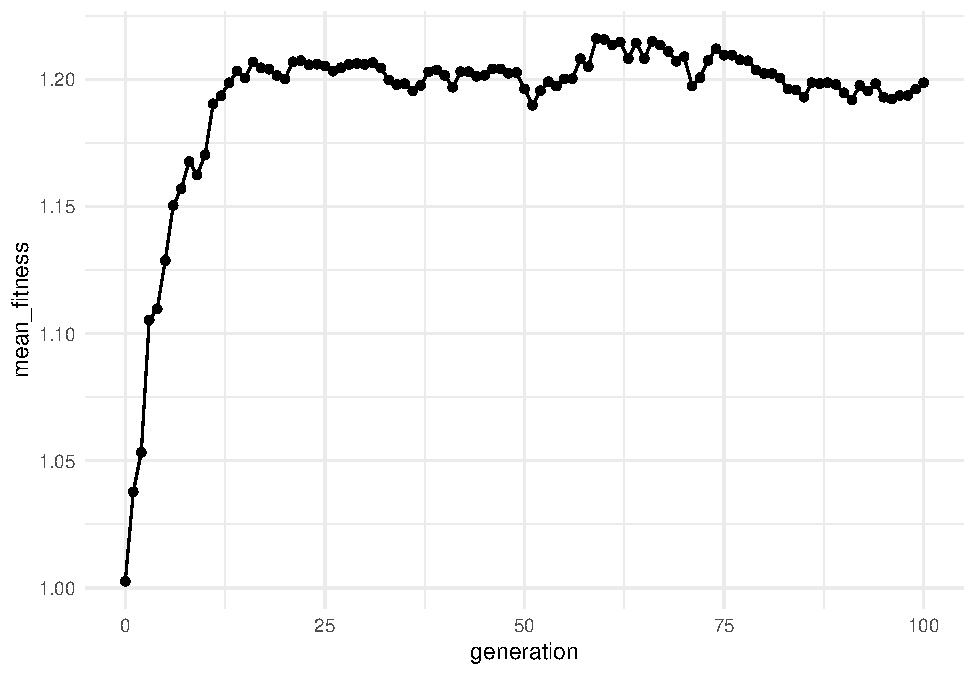
\includegraphics{lifesimulatoR-book_files/lifesimulatoR-book_files/figure-latex/origin-simple-plot-1.pdf}

This plot helps us ask whether the molecular population shows selection-like change over time.

\section{Interpretation of results}\label{interpretation-of-results}

This simulation does not show the actual origin of life. Instead, it demonstrates a simplified principle:

\begin{quote}
If a population has variation, replication, mutation, and selection, then population-level properties can change through time.
\end{quote}

If mean fitness increases, the toy model is showing that some molecular variants are becoming more successful under the model's assumptions.

If diversity changes, the model is showing the balance between two opposing forces:

\begin{itemize}
\tightlist
\item
  mutation introduces new variants,
\item
  selection amplifies successful variants.
\end{itemize}

In a classroom setting, this example can introduce the difference between:

\begin{itemize}
\tightlist
\item
  chemical randomness,
\item
  evolutionary dynamics,
\item
  life-like organization,
\item
  and modern biological life.
\end{itemize}

\section{What this model leaves out}\label{what-this-model-leaves-out}

This simplified model does not include:

\begin{itemize}
\tightlist
\item
  real molecular chemistry,
\item
  RNA folding,
\item
  energy gradients,
\item
  thermodynamics,
\item
  mineral surfaces,
\item
  wet-dry cycles,
\item
  environmental change,
\item
  spatial structure,
\item
  membranes or compartments,
\item
  metabolism.
\end{itemize}

These omissions are intentional. The purpose of the model is to isolate a few basic ideas and make them easy to explore.

Later chapters introduce additional concepts such as diversity metrics, protocells, and autocatalytic networks.

\section{How this chapter connects to the rest of the book}\label{how-this-chapter-connects-to-the-rest-of-the-book}

This chapter introduces the central problem: how non-living systems might begin to show life-like behaviour.

The next chapters explore this question from different angles:

\begin{itemize}
\tightlist
\item
  \textbf{Prebiotic Chemistry and Molecular Pools}: Where does molecular variation come from?
\item
  \textbf{Molecular Evolution}: How do mutation, replication, and selection change populations?
\item
  \textbf{Diversity and Complexity}: How can we measure variation and organization?
\item
  \textbf{Protocells}: How can compartments create individuality?
\item
  \textbf{Autocatalytic Networks}: How can systems become self-reinforcing?
\end{itemize}

\section{Reflection questions}\label{reflection-questions}

\begin{enumerate}
\def\labelenumi{\arabic{enumi}.}
\tightlist
\item
  Which features of life are represented in this simple simulation?
\item
  Which features are missing?
\item
  Could evolution begin before cells existed?
\item
  Could selection act on molecules, compartments, or networks?
\item
  Does increasing fitness imply increasing complexity?
\item
  What would need to be added to make this model more chemically realistic?
\end{enumerate}

\chapter{Prebiotic Chemistry and Molecular Pools}\label{prebiotic-chemistry-and-molecular-pools}

\section{Why Prebiotic Chemistry Matters}\label{why-prebiotic-chemistry-matters}

Before life could evolve, the building blocks of life had to exist. The first challenge in any origin-of-life theory is therefore not replication, selection, or evolution, but chemistry.

Modern organisms depend on a remarkable collection of molecules, including amino acids, nucleotides, lipids, sugars, proteins, RNA, and DNA. Yet before life existed, none of these molecules were being produced by biological systems. They had to arise through natural physical and chemical processes operating on the early Earth.

This raises one of the central questions of origin-of-life research:

\begin{quote}
Could the early Earth naturally produce the molecular building blocks required for life?
\end{quote}

Understanding how simple chemistry could generate increasingly complex molecular systems is the starting point for nearly every scientific theory of abiogenesis.

\section{The Early Earth}\label{the-early-earth}

The Earth formed approximately 4.5 billion years ago. During its first several hundred million years, conditions were dramatically different from those we experience today.

Scientists believe the young Earth experienced:

\begin{itemize}
\tightlist
\item
  Extensive volcanic activity
\item
  Frequent meteorite and comet impacts
\item
  Intense ultraviolet radiation
\item
  A largely oxygen-free atmosphere
\item
  Widespread hydrothermal activity
\item
  Dynamic cycles of evaporation and rainfall
\end{itemize}

Although these conditions appear hostile by modern standards, they may have provided exactly the kinds of energy sources needed to drive complex chemical reactions.

The challenge facing origin-of-life researchers is to determine whether these environments could generate sufficient molecular complexity to eventually produce self-organizing and self-replicating systems.

\section{Sources of Prebiotic Molecules}\label{sources-of-prebiotic-molecules}

Several environments have been proposed as potential locations where prebiotic chemistry may have flourished.

\section{Hydrothermal Vents}\label{hydrothermal-vents}

Hydrothermal vents occur where heated water emerges from Earth's crust into the ocean.

These environments provide:

\begin{itemize}
\tightlist
\item
  Continuous energy flow
\item
  Chemical gradients
\item
  Mineral catalysts
\item
  Stable reaction environments
\end{itemize}

Many metabolism-first theories propose that life originated in hydrothermal vent systems because they naturally maintain chemical disequilibria that can drive reactions.

\section{Shallow Ponds and Tide Pools}\label{shallow-ponds-and-tide-pools}

Another possibility is that life began in shallow bodies of water exposed to repeated wet-dry cycles.

These environments may have advantages such as:

\begin{itemize}
\tightlist
\item
  Concentration of dissolved molecules
\item
  Increased reaction frequency
\item
  Drying phases that encourage polymer formation
\item
  Exposure to sunlight and atmospheric gases
\end{itemize}

Many researchers view wet-dry cycles as particularly important because they may help overcome the dilution problem that affects many aqueous chemical reactions.

\section{Mineral Surfaces}\label{mineral-surfaces}

Minerals may have played a crucial role in organizing prebiotic chemistry.

Clay minerals and other surfaces can:

\begin{itemize}
\tightlist
\item
  Concentrate molecules
\item
  Catalyze reactions
\item
  Provide structural templates
\item
  Protect molecules from degradation
\end{itemize}

Some origin-of-life models propose that minerals served as scaffolds upon which increasingly complex chemistry emerged.

\section{Ice Environments}\label{ice-environments}

Cold environments may seem unlikely places for life to begin, but they offer several potential advantages.

Ice can:

\begin{itemize}
\tightlist
\item
  Protect fragile molecules
\item
  Slow destructive reactions
\item
  Concentrate dissolved substances in microscopic channels
\item
  Stabilize reaction intermediates
\end{itemize}

As a result, frozen environments are now considered plausible locations for important prebiotic processes.

\section{The Miller--Urey Experiment}\label{the-millerurey-experiment}

One of the most famous experiments in origin-of-life research was conducted by Stanley Miller and Harold Urey in 1953.

The experiment attempted to simulate conditions believed to resemble the early Earth. A mixture of gases was exposed to electrical sparks representing lightning.

After only a short period, the apparatus produced several amino acids---the building blocks of proteins.

The significance of the experiment was profound:

\begin{quote}
Biologically relevant molecules can arise spontaneously from non-living chemistry.
\end{quote}

Although modern interpretations of the early atmosphere differ from those originally assumed by Miller and Urey, the experiment demonstrated an important principle that remains central to origin-of-life research today.

\section{From Molecules to Molecular Pools}\label{from-molecules-to-molecular-pools}

Prebiotic chemistry likely did not produce isolated molecules one at a time. Instead, it probably generated complex mixtures containing many different molecular species.

These collections are often referred to as \textbf{prebiotic molecular pools}.

A molecular pool may contain:

\begin{itemize}
\tightlist
\item
  Thousands of distinct molecules
\item
  Molecules of varying lengths
\item
  Molecules with different stabilities
\item
  Molecules with different catalytic properties
\item
  Molecules interacting in complex ways
\end{itemize}

Most origin-of-life theories begin with some form of molecular pool because evolution requires variation.

Without variation, there can be no selection.

\section{Chemical Space}\label{chemical-space}

One of the most important concepts in origin-of-life research is \textbf{chemical space}.

Chemical space refers to the enormous set of all possible molecular structures that could exist.

Even simple molecules can generate enormous numbers of possible combinations.

For example, a symbolic sequence built from four symbols has:

\begin{itemize}
\tightlist
\item
  4 possible sequences of length 1
\item
  16 possible sequences of length 2
\item
  64 possible sequences of length 3
\item
  1,048,576 possible sequences of length 10
\end{itemize}

As sequence length increases, the number of possible structures grows exponentially.

This creates both an opportunity and a challenge:

\begin{itemize}
\tightlist
\item
  Large chemical spaces provide many possibilities.
\item
  Large chemical spaces are difficult to search efficiently.
\end{itemize}

A central question in origin-of-life research is how prebiotic systems explored chemical space well enough to discover useful molecular structures.

\section{\texorpdfstring{Conceptual Model in \texttt{lifesimulatoR}}{Conceptual Model in lifesimulatoR}}\label{conceptual-model-in-lifesimulator}

Modeling actual prebiotic chemistry requires sophisticated physical chemistry and reaction-network simulations.

To make the concepts more accessible, \texttt{lifesimulatoR} uses a simplified representation.

Instead of real molecules, symbolic molecular sequences are generated from a chosen alphabet.

For example:

\begin{Shaded}
\begin{Highlighting}[]
\FunctionTok{library}\NormalTok{(lifesimulatoR)}

\NormalTok{pool }\OtherTok{\textless{}{-}} \FunctionTok{create\_prebiotic\_pool}\NormalTok{(}
  \AttributeTok{n\_molecules =} \DecValTok{50}\NormalTok{,}
  \AttributeTok{alphabet =} \FunctionTok{c}\NormalTok{(}\StringTok{"A"}\NormalTok{, }\StringTok{"U"}\NormalTok{, }\StringTok{"G"}\NormalTok{, }\StringTok{"C"}\NormalTok{),}
  \AttributeTok{min\_length =} \DecValTok{5}\NormalTok{,}
  \AttributeTok{max\_length =} \DecValTok{15}\NormalTok{,}
  \AttributeTok{seed =} \DecValTok{123}
\NormalTok{)}

\FunctionTok{head}\NormalTok{(pool)}
\end{Highlighting}
\end{Shaded}

Each sequence represents a symbolic molecule.

Although these sequences are not chemically realistic, they allow us to explore concepts such as:

\begin{itemize}
\tightlist
\item
  Diversity
\item
  Mutation
\item
  Selection
\item
  Replication
\item
  Complexity
\item
  Evolutionary dynamics
\end{itemize}

The key modeling idea is:

\begin{quote}
Before selection can act, variation must exist.
\end{quote}

\section{Creating a Prebiotic Molecular Pool}\label{creating-a-prebiotic-molecular-pool}

The function \texttt{create\_prebiotic\_pool()} generates an initial collection of symbolic molecules.

\begin{Shaded}
\begin{Highlighting}[]
\NormalTok{pool }\OtherTok{\textless{}{-}} \FunctionTok{create\_prebiotic\_pool}\NormalTok{(}
  \AttributeTok{n\_molecules =} \DecValTok{50}\NormalTok{,}
  \AttributeTok{alphabet =} \FunctionTok{c}\NormalTok{(}\StringTok{"A"}\NormalTok{, }\StringTok{"U"}\NormalTok{, }\StringTok{"G"}\NormalTok{, }\StringTok{"C"}\NormalTok{),}
  \AttributeTok{min\_length =} \DecValTok{5}\NormalTok{,}
  \AttributeTok{max\_length =} \DecValTok{15}\NormalTok{,}
  \AttributeTok{seed =} \DecValTok{123}
\NormalTok{)}

\FunctionTok{head}\NormalTok{(pool)}
\end{Highlighting}
\end{Shaded}

Each sequence is generated randomly within the specified constraints.

The resulting pool acts as the starting point for later simulations involving mutation, replication, and selection.

\section{Exploring Molecular Diversity}\label{exploring-molecular-diversity}

We can inspect some basic characteristics of the pool.

\begin{Shaded}
\begin{Highlighting}[]
\FunctionTok{data.frame}\NormalTok{(}
  \AttributeTok{molecule =}\NormalTok{ pool[}\DecValTok{1}\SpecialCharTok{:}\DecValTok{10}\NormalTok{],}
  \AttributeTok{length =} \FunctionTok{nchar}\NormalTok{(pool[}\DecValTok{1}\SpecialCharTok{:}\DecValTok{10}\NormalTok{])}
\NormalTok{)}
\end{Highlighting}
\end{Shaded}

Immediately we observe variation among molecules.

Some are longer than others, and their symbolic compositions differ.

This variation is essential because evolution requires differences among competing entities.

\section{Exploring Chemical Space with Different Pools}\label{exploring-chemical-space-with-different-pools}

Changing model parameters changes the size of the symbolic chemical space.

\begin{Shaded}
\begin{Highlighting}[]
\NormalTok{small\_pool }\OtherTok{\textless{}{-}} \FunctionTok{create\_prebiotic\_pool}\NormalTok{(}
  \AttributeTok{n\_molecules =} \DecValTok{10}\NormalTok{,}
  \AttributeTok{min\_length =} \DecValTok{3}\NormalTok{,}
  \AttributeTok{max\_length =} \DecValTok{6}\NormalTok{,}
  \AttributeTok{seed =} \DecValTok{123}
\NormalTok{)}

\NormalTok{large\_pool }\OtherTok{\textless{}{-}} \FunctionTok{create\_prebiotic\_pool}\NormalTok{(}
  \AttributeTok{n\_molecules =} \DecValTok{100}\NormalTok{,}
  \AttributeTok{min\_length =} \DecValTok{8}\NormalTok{,}
  \AttributeTok{max\_length =} \DecValTok{20}\NormalTok{,}
  \AttributeTok{seed =} \DecValTok{123}
\NormalTok{)}

\FunctionTok{length}\NormalTok{(small\_pool)}
\FunctionTok{length}\NormalTok{(large\_pool)}
\end{Highlighting}
\end{Shaded}

Larger pools contain more variation and potentially more opportunities for later evolutionary processes.

Longer molecules also allow more complex symbolic structures to emerge.

\section{Why the Starting Pool Matters}\label{why-the-starting-pool-matters}

The initial molecular pool influences everything that follows.

A larger and more diverse pool may:

\begin{itemize}
\tightlist
\item
  Explore more possibilities
\item
  Generate more novel variants
\item
  Increase opportunities for interaction
\item
  Improve the chances of producing useful structures
\end{itemize}

However, diversity alone is not enough.

A completely random collection of molecules may contain enormous diversity while lacking any ability to persist, replicate, or evolve.

This highlights an important distinction:

\begin{quote}
Diversity provides possibilities, but organization creates life-like behaviour.
\end{quote}

\section{Limitations of the Model}\label{limitations-of-the-model}

The symbolic molecules generated by \texttt{lifesimulatoR} are educational abstractions.

They do not include:

\begin{itemize}
\tightlist
\item
  Molecular structure
\item
  Folding dynamics
\item
  Catalytic activity
\item
  Reaction kinetics
\item
  Energy constraints
\item
  Environmental interactions
\item
  Thermodynamic limitations
\end{itemize}

Consequently, the simulations should not be interpreted as realistic models of prebiotic chemistry.

Instead, they serve as conceptual tools for understanding the logic of variation, diversity, and emergence.

\section{Looking Ahead}\label{looking-ahead}

A prebiotic molecular pool provides the raw material from which more complex systems may emerge.

However, variation alone does not create evolution.

The next question is:

\begin{quote}
What happens when molecules begin to replicate, mutate, and compete?
\end{quote}

The next chapter explores molecular evolution and investigates how replication, mutation, and selection can transform a molecular population over time.

\section{Reflection Questions}\label{reflection-questions-1}

\begin{enumerate}
\def\labelenumi{\arabic{enumi}.}
\tightlist
\item
  Which prebiotic environment do you think provides the most plausible setting for the origin of life? Why?
\item
  Is molecular diversity alone sufficient for life to emerge?
\item
  What challenges arise when searching extremely large chemical spaces?
\item
  How might mineral surfaces influence prebiotic chemistry?
\item
  What advantages might wet-dry cycles provide compared with deep-ocean environments?
\item
  What important aspects of real chemistry are omitted by symbolic molecular models?
\item
  Could multiple origin-of-life environments have contributed simultaneously to the emergence of life?
\item
  How might future simulations better represent real prebiotic chemistry?
\end{enumerate}

\chapter{Molecular Evolution}\label{molecular-evolution}

\section{Why Molecular Evolution Matters}\label{why-molecular-evolution-matters}

One of the central questions in origin-of-life research is how simple chemistry became capable of evolution.

Modern biological evolution depends on three fundamental ingredients:

\begin{itemize}
\tightlist
\item
  Information
\item
  Replication
\item
  Variation
\end{itemize}

Today these functions are carried out primarily by DNA, RNA, and proteins. However, before modern cells existed, simpler molecular systems may have possessed primitive versions of these capabilities.

Molecular evolution studies how populations of molecules change through time when information is copied imperfectly and some variants become more successful than others.

Understanding molecular evolution helps bridge the gap between prebiotic chemistry and the emergence of life.

\section{From Prebiotic Chemistry to Evolution}\label{from-prebiotic-chemistry-to-evolution}

The previous chapter introduced prebiotic molecular pools. These pools contain diverse molecules that may have formed through natural chemical processes on the early Earth.

Diversity alone, however, is not sufficient for evolution.

For evolution to occur:

\begin{enumerate}
\def\labelenumi{\arabic{enumi}.}
\tightlist
\item
  Molecules must differ from one another.
\item
  Some molecules must persist or reproduce more successfully than others.
\item
  Information must be transmitted between generations.
\item
  New variants must appear.
\item
  Successful variants must become more common through time.
\end{enumerate}

When these conditions are satisfied, populations can evolve.

This transition from chemistry to evolution represents one of the most important steps in the origin of life.

\section{The RNA World Hypothesis}\label{the-rna-world-hypothesis}

One of the most influential origin-of-life theories is the RNA World hypothesis.

The central idea is that early life may have been based primarily on RNA-like molecules.

RNA is particularly interesting because it can perform two critical functions:

\begin{itemize}
\tightlist
\item
  Store information
\item
  Catalyze chemical reactions
\end{itemize}

Modern life separates these functions among DNA, RNA, and proteins. The RNA World hypothesis proposes that earlier biological systems may have relied on a single class of molecules capable of doing both.

If correct, evolution may have begun before cells, genomes, and proteins existed.

Although the RNA World remains one of the leading hypotheses, researchers continue to investigate alternative and complementary explanations involving metabolism, compartments, and autocatalytic networks.

\section{Information and Heredity}\label{information-and-heredity}

Evolution requires information.

In biological systems, information refers to patterns that can be copied and transmitted.

For example:

\begin{Shaded}
\begin{Highlighting}[]
\NormalTok{AUGCAUGCAUGC}
\end{Highlighting}
\end{Shaded}

contains information because the arrangement of symbols matters.

When sequences are copied, information is inherited. When copying errors occur, variation is introduced.

The interaction between heredity and variation forms the foundation of evolution.

Without heredity, successful innovations would be lost. Without variation, populations could not adapt or explore new possibilities.

\section{Conceptual Model}\label{conceptual-model-1}

In \texttt{lifesimulatoR}, molecular evolution is represented using symbolic molecular sequences.

The model contains five major processes:

\begin{enumerate}
\def\labelenumi{\arabic{enumi}.}
\tightlist
\item
  Molecular populations
\item
  Fitness evaluation
\item
  Replication
\item
  Mutation
\item
  Selection
\end{enumerate}

Together, these processes generate evolutionary dynamics.

Although simplified, the model captures the essential logic underlying evolutionary change.

\section{Creating a Molecular Population}\label{creating-a-molecular-population}

Evolution begins with a population of molecules.

\begin{Shaded}
\begin{Highlighting}[]
\NormalTok{pool }\OtherTok{\textless{}{-}} \FunctionTok{create\_prebiotic\_pool}\NormalTok{(}
  \AttributeTok{n\_molecules =} \DecValTok{50}\NormalTok{,}
  \AttributeTok{alphabet =} \FunctionTok{c}\NormalTok{(}\StringTok{"A"}\NormalTok{, }\StringTok{"U"}\NormalTok{, }\StringTok{"G"}\NormalTok{, }\StringTok{"C"}\NormalTok{),}
  \AttributeTok{min\_length =} \DecValTok{5}\NormalTok{,}
  \AttributeTok{max\_length =} \DecValTok{15}\NormalTok{,}
  \AttributeTok{seed =} \DecValTok{123}
\NormalTok{)}

\FunctionTok{cat}\NormalTok{(}\FunctionTok{head}\NormalTok{(pool), }\AttributeTok{sep =} \StringTok{"}\SpecialCharTok{\textbackslash{}n}\StringTok{"}\NormalTok{)}
\end{Highlighting}
\end{Shaded}

\begin{verbatim}
## UGUUUGA
## UUAUGCAG
## ACAAAGCUGUAUGCU
## GGACG
## AGAAUGGCAGAGCU
## UAACCGAUAAGAU
\end{verbatim}

Each sequence represents a symbolic molecule.

Although these molecules are simplified abstractions, they allow us to explore the logic of molecular evolution.

\section{Molecular Fitness}\label{molecular-fitness}

Not all molecules are equally successful.

The concept of fitness attempts to capture how likely a molecule is to persist or contribute descendants to future generations.

In real chemistry, fitness may depend on factors such as:

\begin{itemize}
\tightlist
\item
  Stability
\item
  Catalytic activity
\item
  Replication efficiency
\item
  Environmental conditions
\item
  Resource availability
\end{itemize}

In \texttt{lifesimulatoR}, fitness is represented using a simplified scoring function.

\begin{Shaded}
\begin{Highlighting}[]
\NormalTok{molecules }\OtherTok{\textless{}{-}} \FunctionTok{c}\NormalTok{(}
  \StringTok{"AUGC"}\NormalTok{,}
  \StringTok{"AAAAUUUU"}\NormalTok{,}
  \StringTok{"GCGCGC"}\NormalTok{,}
  \StringTok{"AUAUAUAUAUAU"}
\NormalTok{)}

\NormalTok{fitness }\OtherTok{\textless{}{-}} \FunctionTok{molecule\_fitness}\NormalTok{(molecules)}

\FunctionTok{data.frame}\NormalTok{(}
  \AttributeTok{molecule =}\NormalTok{ molecules,}
  \AttributeTok{fitness =}\NormalTok{ fitness}
\NormalTok{)}
\end{Highlighting}
\end{Shaded}

\begin{verbatim}
##       molecule   fitness
## 1         AUGC 0.6993290
## 2     AAAAUUUU 1.0687308
## 3       GCGCGC 0.8876282
## 4 AUAUAUAUAUAU 1.2500000
\end{verbatim}

\section{Fitness Landscapes}\label{fitness-landscapes}

Evolution is often visualized using the concept of a fitness landscape.

A fitness landscape maps molecular structures to fitness values.

\begin{itemize}
\tightlist
\item
  High-fitness molecules occupy peaks.
\item
  Low-fitness molecules occupy valleys.
\item
  Mutation moves populations through the landscape.
\item
  Selection tends to push populations toward higher-fitness regions.
\end{itemize}

Although fitness landscapes are simplified conceptual tools, they help explain how populations can gradually become better adapted.

A useful way to think about evolution is as a search process moving through a landscape of possibilities.

\section{Replication}\label{replication}

Replication is the process by which molecules produce copies of themselves.

Without replication, successful molecules cannot become more common.

\begin{Shaded}
\begin{Highlighting}[]
\NormalTok{next\_generation }\OtherTok{\textless{}{-}} \FunctionTok{replicate\_molecules}\NormalTok{(}
  \AttributeTok{molecules =}\NormalTok{ molecules,}
  \AttributeTok{n\_molecules =} \DecValTok{20}\NormalTok{,}
  \AttributeTok{selection\_strength =} \DecValTok{1}
\NormalTok{)}

\FunctionTok{cat}\NormalTok{(}\FunctionTok{head}\NormalTok{(next\_generation), }\AttributeTok{sep =} \StringTok{"}\SpecialCharTok{\textbackslash{}n}\StringTok{"}\NormalTok{)}
\end{Highlighting}
\end{Shaded}

\begin{verbatim}
## AAAAUUUU
## AAAAUUUU
## AUGC
## AUAUAUAUAUAU
## AUAUAUAUAUAU
## GCGCGC
\end{verbatim}

Replication allows information to persist through time.

Every evolutionary process depends on some mechanism that preserves information from one generation to the next.

\section{Mutation}\label{mutation}

Mutation introduces novelty into a molecular population.

Without mutation, evolution would eventually stop because no new variants could appear.

\begin{Shaded}
\begin{Highlighting}[]
\NormalTok{original }\OtherTok{\textless{}{-}} \StringTok{"AUGCAUGCAUGC"}

\NormalTok{mutated }\OtherTok{\textless{}{-}} \FunctionTok{mutate\_sequence}\NormalTok{(}
  \AttributeTok{sequence =}\NormalTok{ original,}
  \AttributeTok{alphabet =} \FunctionTok{c}\NormalTok{(}\StringTok{"A"}\NormalTok{, }\StringTok{"U"}\NormalTok{, }\StringTok{"G"}\NormalTok{, }\StringTok{"C"}\NormalTok{),}
  \AttributeTok{mutation\_rate =} \FloatTok{0.05}
\NormalTok{)}

\FunctionTok{data.frame}\NormalTok{(}
  \AttributeTok{original =}\NormalTok{ original,}
  \AttributeTok{mutated =}\NormalTok{ mutated}
\NormalTok{)}
\end{Highlighting}
\end{Shaded}

\begin{verbatim}
##       original      mutated
## 1 AUGCAUGCAUGC AUGGAUGCGUGC
\end{verbatim}

Mutation generates diversity, but excessive mutation can also destroy information.

\section{Mutation Rate and the Evolutionary Trade-Off}\label{mutation-rate-and-the-evolutionary-trade-off}

Mutation creates one of evolution's most important trade-offs.

Low mutation rates:

\begin{itemize}
\tightlist
\item
  Preserve information
\item
  Limit innovation
\end{itemize}

High mutation rates:

\begin{itemize}
\tightlist
\item
  Generate novelty
\item
  Risk destroying successful structures
\end{itemize}

Evolution requires a balance between stability and innovation.

Too little mutation limits exploration. Too much mutation prevents successful information from being preserved.

\section{The Error Threshold}\label{the-error-threshold}

One of the most important concepts in molecular evolution is the error threshold.

If mutation rates become too high:

\begin{itemize}
\tightlist
\item
  Successful sequences cannot be preserved.
\item
  Information is lost.
\item
  Selection becomes ineffective.
\end{itemize}

This idea is closely associated with Eigen's work on early replicators.

A major challenge for the earliest evolving systems may have been maintaining enough copying accuracy to preserve information while still generating useful variation.

The error threshold remains a central concept in studies of the origin of life.

\section{Selection}\label{selection}

Selection occurs whenever some molecules contribute more descendants than others.

Selection is not a conscious process. It emerges automatically whenever certain variants persist or replicate more successfully.

In the simulation:

\begin{itemize}
\tightlist
\item
  Weak selection produces nearly neutral evolution.
\item
  Strong selection favors fitter molecules more strongly.
\end{itemize}

Selection acts as a filter on variation.

Mutation generates possibilities. Selection determines which possibilities persist.

\section{Evolving One Generation}\label{evolving-one-generation}

Mutation, replication, and selection can be combined into a single evolutionary step.

\begin{Shaded}
\begin{Highlighting}[]
\NormalTok{next\_generation }\OtherTok{\textless{}{-}} \FunctionTok{evolve\_generation}\NormalTok{(}
  \AttributeTok{molecules =}\NormalTok{ pool,}
  \AttributeTok{mutation\_rate =} \FloatTok{0.02}\NormalTok{,}
  \AttributeTok{selection\_strength =} \DecValTok{1}
\NormalTok{)}

\FunctionTok{head}\NormalTok{(next\_generation)}
\end{Highlighting}
\end{Shaded}

\begin{verbatim}
## [1] "UUAUGCAG"     "GCCGUGC"      "UUCACUACCA"   "UAUGCAAC"     "UCUGAUCACUAC" "UUUGCGGUAUC"
\end{verbatim}

This represents one generation of molecular evolution.

Repeated application of this process can produce long-term evolutionary change.

\section{Simulating Molecular Evolution}\label{simulating-molecular-evolution}

The full simulation repeatedly applies mutation, replication, and selection across many generations.

\begin{Shaded}
\begin{Highlighting}[]
\NormalTok{sim }\OtherTok{\textless{}{-}} \FunctionTok{simulate\_abiogenesis}\NormalTok{(}
  \AttributeTok{n\_molecules =} \DecValTok{100}\NormalTok{,}
  \AttributeTok{generations =} \DecValTok{200}\NormalTok{,}
  \AttributeTok{mutation\_rate =} \FloatTok{0.02}\NormalTok{,}
  \AttributeTok{selection\_strength =} \DecValTok{1}\NormalTok{,}
  \AttributeTok{seed =} \DecValTok{123}
\NormalTok{)}

\FunctionTok{head}\NormalTok{(sim)}
\end{Highlighting}
\end{Shaded}

\begin{verbatim}
## # A tibble: 6 x 6
##   generation n_molecules mean_length mean_fitness diversity max_fitness
##        <int>       <int>       <dbl>        <dbl>     <int>       <dbl>
## 1          0         100        12.6         1.00       100        1.25
## 2          1         100        12.7         1.04        67        1.25
## 3          2         100        12.3         1.05        61        1.25
## 4          3         100        12.3         1.11        61        1.25
## 5          4         100        12.5         1.11        48        1.25
## 6          5         100        12.8         1.13        53        1.25
\end{verbatim}

\section{Visualizing Fitness Through Time}\label{visualizing-fitness-through-time}

\begin{Shaded}
\begin{Highlighting}[]
\FunctionTok{plot\_simulation}\NormalTok{(}
\NormalTok{  sim,}
  \AttributeTok{x =} \StringTok{"generation"}\NormalTok{,}
  \AttributeTok{y =} \StringTok{"mean\_fitness"}
\NormalTok{)}
\end{Highlighting}
\end{Shaded}

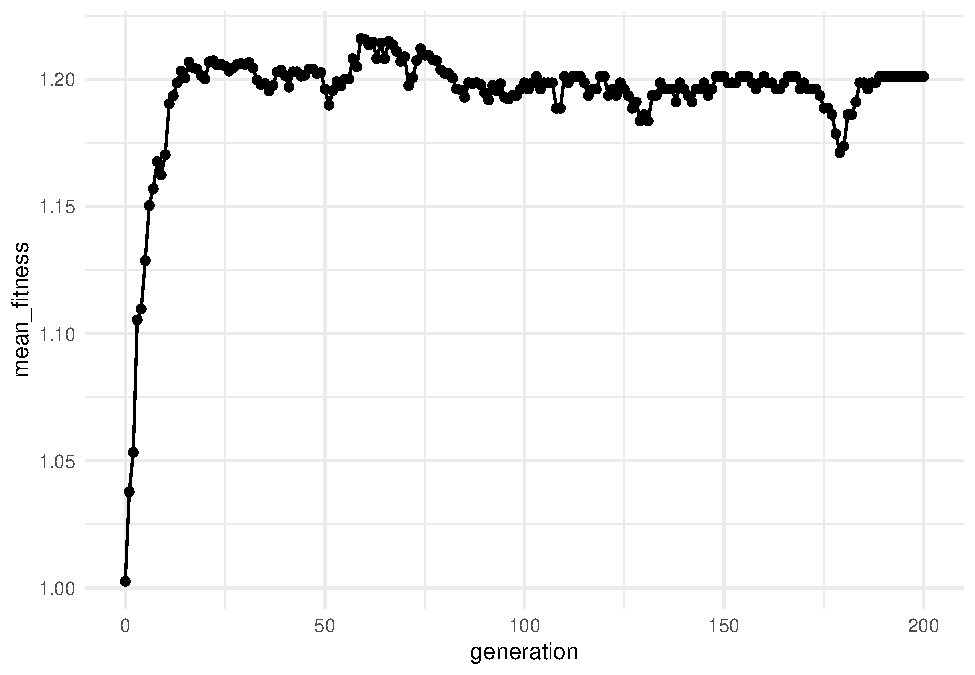
\includegraphics{lifesimulatoR-book_files/lifesimulatoR-book_files/figure-latex/ch03-fitness-plot-1.pdf}

This plot helps reveal whether fitter molecular variants become more common through time.

\section{Visualizing Diversity Through Time}\label{visualizing-diversity-through-time}

\begin{Shaded}
\begin{Highlighting}[]
\FunctionTok{plot\_simulation}\NormalTok{(}
\NormalTok{  sim,}
  \AttributeTok{x =} \StringTok{"generation"}\NormalTok{,}
  \AttributeTok{y =} \StringTok{"diversity"}
\NormalTok{)}
\end{Highlighting}
\end{Shaded}

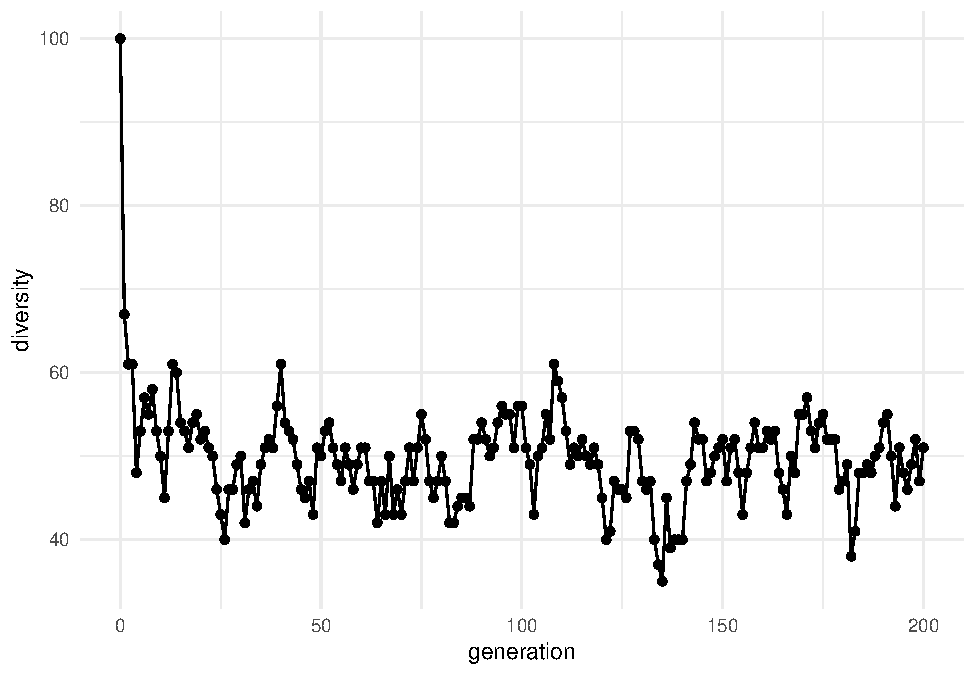
\includegraphics{lifesimulatoR-book_files/lifesimulatoR-book_files/figure-latex/ch03-diversity-plot-1.pdf}

Diversity provides information about how broadly the population is exploring sequence space.

\section{Interpreting Simulation Results}\label{interpreting-simulation-results}

Several outcomes are possible.

\subsection{Increasing Fitness}\label{increasing-fitness}

May indicate:

\begin{itemize}
\tightlist
\item
  Successful variants becoming more common
\item
  Selection acting effectively
\end{itemize}

\subsection{Increasing Diversity}\label{increasing-diversity}

May indicate:

\begin{itemize}
\tightlist
\item
  Exploration of new sequence space
\item
  Significant mutation activity
\end{itemize}

\subsection{Decreasing Diversity}\label{decreasing-diversity}

May indicate:

\begin{itemize}
\tightlist
\item
  Dominance by a small number of successful variants
\item
  Strong selective pressures
\end{itemize}

\subsection{Stable Values}\label{stable-values}

May indicate:

\begin{itemize}
\tightlist
\item
  Equilibrium under the assumptions of the model
\item
  Balance between mutation and selection
\end{itemize}

\section{Evolution as Information Processing}\label{evolution-as-information-processing}

A useful way to think about evolution is as a process that accumulates information.

Mutation generates possibilities.

Selection filters possibilities.

Replication preserves successful patterns.

Together, these processes can gradually increase organization within a population.

From this perspective, evolution can be viewed as a mechanism for discovering and preserving useful information.

\section{Limitations of the Model}\label{limitations-of-the-model-1}

This model intentionally omits many aspects of real chemistry, including:

\begin{itemize}
\tightlist
\item
  RNA folding
\item
  Catalytic mechanisms
\item
  Resource competition
\item
  Environmental fluctuations
\item
  Thermodynamics
\item
  Spatial organization
\item
  Membrane compartmentalization
\item
  Metabolic networks
\end{itemize}

The goal is conceptual clarity rather than chemical realism.

\section{Connections to Later Chapters}\label{connections-to-later-chapters}

Molecular evolution addresses how information-bearing molecules may change through time.

However, life requires more than information.

Living systems also require:

\begin{itemize}
\tightlist
\item
  Compartments
\item
  Networks
\item
  Energy flow
\item
  Self-maintenance
\end{itemize}

The next chapters explore diversity, complexity, protocells, and autocatalytic networks to examine how these additional ingredients may have contributed to the emergence of life.

\section{Key Takeaways}\label{key-takeaways}

\begin{itemize}
\tightlist
\item
  Molecular evolution may have preceded modern cellular life.
\item
  The RNA World hypothesis provides one possible framework for early evolution.
\item
  Replication, mutation, and selection generate evolutionary change.
\item
  Fitness landscapes help explain adaptation.
\item
  Excessive mutation can destroy information through the error threshold.
\item
  Evolution can be viewed as an information-processing process.
\item
  Molecular populations can accumulate organization through repeated cycles of variation and selection.
\item
  \texttt{lifesimulatoR} provides simplified computational models for exploring these concepts.
\end{itemize}

\section{Suggested Readings}\label{suggested-readings}

\begin{itemize}
\tightlist
\item
  Eigen, M. (1971). \emph{Self-Organization of Matter and the Evolution of Biological Macromolecules.}
\item
  Gilbert, W. (1986). \emph{The RNA World.}
\item
  Joyce, G. F. (2002). \emph{The Antiquity of RNA-Based Evolution.}
\item
  Maynard Smith, J., \& Szathmáry, E. (1999). \emph{The Origins of Life.}
\item
  Kauffman, S. (1993). \emph{The Origins of Order.}
\end{itemize}

\section{Reflection Questions}\label{reflection-questions-2}

\begin{enumerate}
\def\labelenumi{\arabic{enumi}.}
\tightlist
\item
  Why is information essential for evolution?
\item
  Could evolution occur before cells existed?
\item
  What limits the mutation rate of early replicators?
\item
  How does the concept of a fitness landscape help explain adaptation?
\item
  Is higher fitness always associated with greater complexity?
\item
  Could molecular evolution begin before metabolism?
\item
  What additional mechanisms are needed to transform evolving molecules into living systems?
\item
  What aspects of molecular evolution are not captured by symbolic sequence models?
\item
  Can selection create information, or only preserve it?
\item
  What role might molecular evolution have played in the transition from chemistry to biology?
\end{enumerate}

\chapter{Diversity, Entropy, and Complexity}\label{diversity-entropy-and-complexity}

\section{Why Diversity Matters}\label{why-diversity-matters}

One of the most important questions in origin-of-life research is how simple chemical systems became sufficiently complex to give rise to life.

A key ingredient in this process is diversity.

A system containing many different molecular types can explore more possibilities than a system containing only a few molecular types. Diversity creates opportunities for new interactions, new structures, and potentially new functions.

However, diversity alone is not the same as life.

A completely random mixture of molecules may be highly diverse but possess no organization, no persistence, and no capacity for evolution.

This distinction is important:

\begin{quote}
Diversity creates possibilities, but organization creates life-like behaviour.
\end{quote}

Understanding the relationship between diversity, entropy, and complexity helps us investigate how chemical systems may transition from randomness to biological organization.

\section{Diversity in Origin-of-Life Research}\label{diversity-in-origin-of-life-research}

Many origin-of-life theories rely on diversity as a source of innovation.

Examples include:

\begin{itemize}
\tightlist
\item
  Diverse molecular pools exploring chemical space
\item
  Diverse catalytic networks generating new reactions
\item
  Diverse protocell populations competing for resources
\item
  Diverse replicators undergoing selection
\end{itemize}

Without variation, evolution cannot occur.

Without diversity, selection has nothing to act upon.

Consequently, diversity is often viewed as the raw material of evolutionary change.

\section{What Is Entropy?}\label{what-is-entropy}

Entropy is a concept used in several scientific disciplines.

In thermodynamics, entropy is often associated with disorder and the number of possible microscopic arrangements of a system.

In information theory, entropy measures uncertainty or unpredictability.

Although these definitions are related, they are not identical.

This chapter focuses primarily on \textbf{Shannon entropy}, which is widely used to quantify diversity in populations.

\section{Shannon Entropy}\label{shannon-entropy}

Claude Shannon introduced entropy in 1948 as a measure of information and uncertainty.

Suppose a population contains several categories with different abundances.

If one category dominates, uncertainty is low because outcomes are predictable.

If abundances are evenly distributed, uncertainty is higher because outcomes are less predictable.

Shannon entropy quantifies this uncertainty.

Higher entropy generally indicates:

\begin{itemize}
\tightlist
\item
  Greater diversity
\item
  More even distributions
\item
  Less predictability
\end{itemize}

Lower entropy generally indicates:

\begin{itemize}
\tightlist
\item
  Less diversity
\item
  Dominance by a few categories
\item
  Greater predictability
\end{itemize}

\section{Conceptual Model}\label{conceptual-model-2}

In \texttt{lifesimulatoR}, diversity can be explored through:

\begin{itemize}
\tightlist
\item
  symbolic molecular populations,
\item
  abundance distributions,
\item
  summary statistics,
\item
  entropy calculations,
\item
  evolutionary simulations.
\end{itemize}

These tools help us examine how diversity changes through time and how diversity interacts with mutation and selection.

\section{Summarizing a Molecular Population}\label{summarizing-a-molecular-population}

Before measuring diversity, it is useful to summarize the molecular population.

\begin{Shaded}
\begin{Highlighting}[]
\NormalTok{molecules }\OtherTok{\textless{}{-}} \FunctionTok{c}\NormalTok{(}
  \StringTok{"AUGC"}\NormalTok{,}
  \StringTok{"AUGC"}\NormalTok{,}
  \StringTok{"UUUU"}\NormalTok{,}
  \StringTok{"GCGCGC"}\NormalTok{,}
  \StringTok{"AUAUAUAUAU"}
\NormalTok{)}

\FunctionTok{summarize\_molecules}\NormalTok{(}
  \AttributeTok{molecules =}\NormalTok{ molecules,}
  \AttributeTok{generation =} \DecValTok{0}
\NormalTok{)}
\end{Highlighting}
\end{Shaded}

\begin{verbatim}
## # A tibble: 1 x 6
##   generation n_molecules mean_length mean_fitness diversity max_fitness
##        <dbl>       <int>       <dbl>        <dbl>     <int>       <dbl>
## 1          0           5         5.6        0.787         4        1.20
\end{verbatim}

The summary may include information such as:

\begin{itemize}
\tightlist
\item
  Number of molecules
\item
  Mean sequence length
\item
  Diversity
\item
  Mean fitness
\item
  Maximum fitness
\end{itemize}

These metrics provide a high-level description of the population.

\section{Measuring Shannon Entropy}\label{measuring-shannon-entropy}

Entropy can be calculated directly from abundance counts.

\begin{Shaded}
\begin{Highlighting}[]
\NormalTok{counts }\OtherTok{\textless{}{-}} \FunctionTok{c}\NormalTok{(}\DecValTok{10}\NormalTok{, }\DecValTok{5}\NormalTok{, }\DecValTok{1}\NormalTok{)}

\FunctionTok{shannon\_entropy}\NormalTok{(counts)}
\end{Highlighting}
\end{Shaded}

\begin{verbatim}
## [1] 1.198192
\end{verbatim}

The result represents the uncertainty associated with randomly selecting an individual from the population.

\section{Comparing Low and High Diversity Systems}\label{comparing-low-and-high-diversity-systems}

Consider two populations.

The first population is dominated by one category.

The second population is evenly distributed.

\begin{Shaded}
\begin{Highlighting}[]
\NormalTok{low\_diversity }\OtherTok{\textless{}{-}} \FunctionTok{c}\NormalTok{(}\DecValTok{100}\NormalTok{, }\DecValTok{1}\NormalTok{, }\DecValTok{1}\NormalTok{, }\DecValTok{1}\NormalTok{)}

\NormalTok{high\_diversity }\OtherTok{\textless{}{-}} \FunctionTok{c}\NormalTok{(}\DecValTok{25}\NormalTok{, }\DecValTok{25}\NormalTok{, }\DecValTok{25}\NormalTok{, }\DecValTok{25}\NormalTok{)}

\FunctionTok{shannon\_entropy}\NormalTok{(low\_diversity)}
\end{Highlighting}
\end{Shaded}

\begin{verbatim}
## [1] 0.2361547
\end{verbatim}

\begin{Shaded}
\begin{Highlighting}[]
\FunctionTok{shannon\_entropy}\NormalTok{(high\_diversity)}
\end{Highlighting}
\end{Shaded}

\begin{verbatim}
## [1] 2
\end{verbatim}

The evenly distributed population has higher entropy because outcomes are less predictable.

This illustrates one of the most important properties of entropy:

\begin{quote}
Entropy increases when abundance is distributed more evenly among categories.
\end{quote}

\section{Diversity Versus Randomness}\label{diversity-versus-randomness}

An important misconception is that high entropy automatically means high complexity.

This is not necessarily true.

Consider three systems:

\subsection{Ordered System}\label{ordered-system}

\begin{Shaded}
\begin{Highlighting}[]
\NormalTok{AAAAAAAAAAAA}
\end{Highlighting}
\end{Shaded}

Characteristics:

\begin{itemize}
\tightlist
\item
  Low diversity
\item
  Low entropy
\item
  Low complexity
\end{itemize}

\subsection{Random System}\label{random-system}

\begin{Shaded}
\begin{Highlighting}[]
\NormalTok{AUGCGAUUGCGA}
\end{Highlighting}
\end{Shaded}

Characteristics:

\begin{itemize}
\tightlist
\item
  High diversity
\item
  High entropy
\item
  Often low organization
\end{itemize}

\subsection{Organized System}\label{organized-system}

\begin{Shaded}
\begin{Highlighting}[]
\NormalTok{Functional replicator}
\end{Highlighting}
\end{Shaded}

Characteristics:

\begin{itemize}
\tightlist
\item
  Moderate diversity
\item
  Structured information
\item
  Potentially high complexity
\end{itemize}

Life appears to occupy a middle ground between complete order and complete randomness.

This idea is central to many theories of emergence and self-organization.

\section{Diversity During Evolution}\label{diversity-during-evolution}

Mutation and selection continually influence diversity.

Mutation tends to create new variants.

Selection tends to amplify successful variants.

The interaction between these forces determines how diversity changes through time.

\begin{Shaded}
\begin{Highlighting}[]
\NormalTok{sim }\OtherTok{\textless{}{-}} \FunctionTok{simulate\_abiogenesis}\NormalTok{(}
  \AttributeTok{n\_molecules =} \DecValTok{100}\NormalTok{,}
  \AttributeTok{generations =} \DecValTok{100}\NormalTok{,}
  \AttributeTok{mutation\_rate =} \FloatTok{0.02}\NormalTok{,}
  \AttributeTok{selection\_strength =} \DecValTok{1}\NormalTok{,}
  \AttributeTok{seed =} \DecValTok{123}
\NormalTok{)}

\FunctionTok{head}\NormalTok{(sim)}
\end{Highlighting}
\end{Shaded}

\begin{verbatim}
## # A tibble: 6 x 6
##   generation n_molecules mean_length mean_fitness diversity max_fitness
##        <int>       <int>       <dbl>        <dbl>     <int>       <dbl>
## 1          0         100        12.6         1.00       100        1.25
## 2          1         100        12.7         1.04        67        1.25
## 3          2         100        12.3         1.05        61        1.25
## 4          3         100        12.3         1.11        61        1.25
## 5          4         100        12.5         1.11        48        1.25
## 6          5         100        12.8         1.13        53        1.25
\end{verbatim}

\section{Visualizing Diversity Through Time}\label{visualizing-diversity-through-time-1}

\begin{Shaded}
\begin{Highlighting}[]
\FunctionTok{plot\_simulation}\NormalTok{(}
\NormalTok{  sim,}
  \AttributeTok{x =} \StringTok{"generation"}\NormalTok{,}
  \AttributeTok{y =} \StringTok{"diversity"}
\NormalTok{)}
\end{Highlighting}
\end{Shaded}

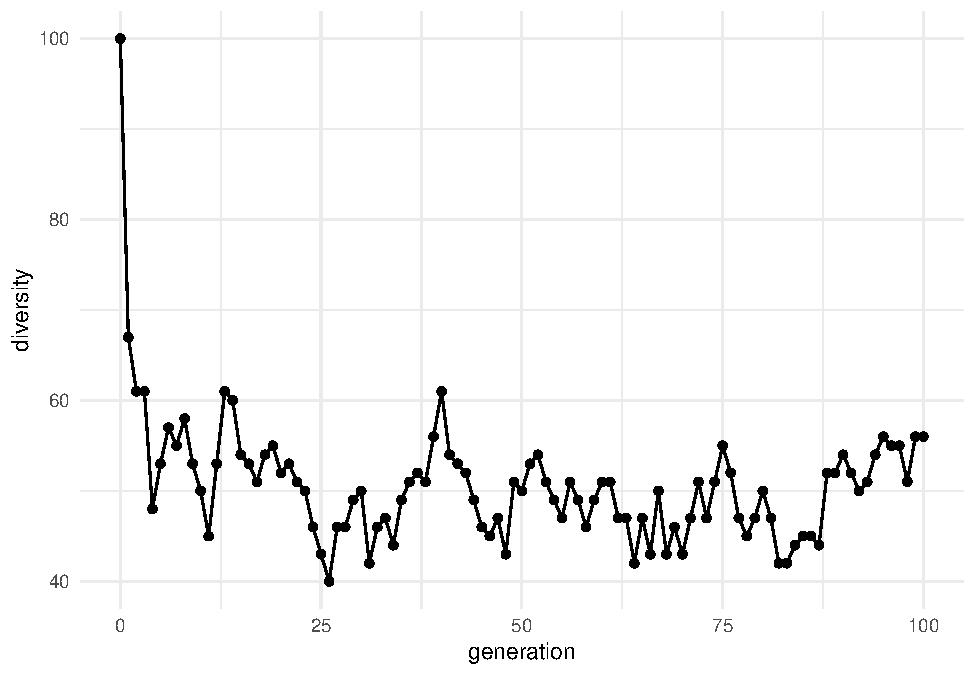
\includegraphics{lifesimulatoR-book_files/lifesimulatoR-book_files/figure-latex/diverse-plot-1.pdf}

This plot allows us to examine how molecular diversity changes throughout the simulation.

\section{Interpreting Diversity Trends}\label{interpreting-diversity-trends}

Several outcomes are possible.

\subsection{Increasing Diversity}\label{increasing-diversity-1}

May indicate:

\begin{itemize}
\tightlist
\item
  Exploration of sequence space
\item
  High mutation rates
\item
  Continued generation of novelty
\end{itemize}

\subsection{Decreasing Diversity}\label{decreasing-diversity-1}

May indicate:

\begin{itemize}
\tightlist
\item
  Strong selection
\item
  Dominance by a small number of successful variants
\item
  Reduced exploration
\end{itemize}

\subsection{Stable Diversity}\label{stable-diversity}

May indicate:

\begin{itemize}
\tightlist
\item
  Balance between mutation and selection
\item
  Dynamic equilibrium
\end{itemize}

No single pattern is inherently better.

Different evolutionary scenarios may produce different diversity trajectories.

\section{Complexity and the Origin of Life}\label{complexity-and-the-origin-of-life}

Complexity is one of the most challenging concepts in science.

A system may be considered complex when:

\begin{itemize}
\tightlist
\item
  Many components interact
\item
  Patterns emerge across multiple scales
\item
  The whole exhibits properties not obvious from the parts
\end{itemize}

Life is often regarded as a complex system because:

\begin{itemize}
\tightlist
\item
  Molecules interact in networks
\item
  Information is stored and transmitted
\item
  Feedback loops exist
\item
  Evolution generates adaptation
\end{itemize}

One of the central challenges in origin-of-life research is explaining how complexity emerged from simpler chemical systems.

\section{Diversity Is Not Enough}\label{diversity-is-not-enough}

Diversity is necessary for evolution, but it is not sufficient.

A highly diverse system may still lack:

\begin{itemize}
\tightlist
\item
  Replication
\item
  Heredity
\item
  Selection
\item
  Compartmentalization
\item
  Self-maintenance
\end{itemize}

Many origin-of-life theories therefore focus on understanding how diversity became organized into increasingly integrated systems.

This transition from diversity to organization may represent one of the most important steps in the emergence of life.

\section{Connections to Other Chapters}\label{connections-to-other-chapters}

This chapter builds upon:

\begin{itemize}
\tightlist
\item
  Prebiotic molecular pools
\item
  Molecular evolution
\end{itemize}

It also prepares the foundation for:

\begin{itemize}
\tightlist
\item
  Protocells
\item
  Autocatalytic networks
\item
  Emergence
\item
  Information theory
\item
  Complexity science
\end{itemize}

These topics explore how diversity becomes structured and how organization emerges from interacting components.

\section{Key Takeaways}\label{key-takeaways-1}

\begin{itemize}
\tightlist
\item
  Diversity provides the variation required for evolution.
\item
  Shannon entropy measures uncertainty and diversity.
\item
  High entropy does not necessarily imply high complexity.
\item
  Mutation tends to increase diversity.
\item
  Selection often reduces diversity.
\item
  Complexity emerges from interactions among components.
\item
  Life appears to occupy a region between complete order and complete randomness.
\item
  Understanding diversity is essential for understanding the origin of life.
\end{itemize}

\section{Suggested Readings}\label{suggested-readings-1}

\begin{itemize}
\tightlist
\item
  Shannon, C. E. (1948). \emph{A Mathematical Theory of Communication.}
\item
  Maynard Smith, J., \& Szathmáry, E. (1999). \emph{The Origins of Life.}
\item
  Kauffman, S. (1993). \emph{The Origins of Order.}
\item
  Adami, C. (2016). \emph{What Is Information?}
\item
  Walker, S. I. (2017). \emph{Origins of Life and Complexity.}
\end{itemize}

\section{Reflection Questions}\label{reflection-questions-3}

\begin{enumerate}
\def\labelenumi{\arabic{enumi}.}
\tightlist
\item
  Is a highly diverse system always more life-like?
\item
  Can selection reduce diversity while increasing organization?
\item
  How is Shannon entropy different from thermodynamic entropy?
\item
  Why is high entropy not necessarily equivalent to high complexity?
\item
  Can complexity emerge without evolution?
\item
  How much diversity is needed before selection becomes effective?
\item
  Could life emerge in a system with very low diversity?
\item
  What additional complexity metrics could be added to future simulations?
\item
  Why does life appear to exist between complete order and complete randomness?
\item
  How might diversity contribute to the emergence of new biological functions?
\end{enumerate}

\chapter{Protocells and Compartmentalization}\label{protocells-and-compartmentalization}

\section{Why Compartments Matter}\label{why-compartments-matter}

One of the greatest challenges facing early life was maintaining organization in a dynamic environment.

Even if useful molecules formed naturally, they faced a fundamental problem:

\begin{itemize}
\tightlist
\item
  molecules diffuse,
\item
  reactions disperse products,
\item
  useful combinations are easily lost.
\end{itemize}

Modern cells solve this problem through membranes that separate internal chemistry from the surrounding environment.

Origin-of-life researchers therefore ask an important question:

\begin{quote}
Could compartmentalization have emerged before modern cells existed?
\end{quote}

Many scientists believe that primitive compartments, known as protocells, may have provided a critical stepping stone between chemistry and biology.

\section{What Is a Protocell?}\label{what-is-a-protocell}

A protocell is a simplified cell-like structure that contains an internal chemical environment separated from the outside world.

Unlike modern cells, protocells do not necessarily possess:

\begin{itemize}
\tightlist
\item
  DNA
\item
  RNA genomes
\item
  proteins
\item
  complex metabolism
\item
  sophisticated membranes
\end{itemize}

Instead, protocells are often envisioned as simple compartments capable of:

\begin{itemize}
\tightlist
\item
  containing molecules,
\item
  growing,
\item
  exchanging materials,
\item
  dividing,
\item
  competing with other compartments.
\end{itemize}

A protocell does not need to be alive in the modern sense to play an important role in origin-of-life theories.

\section{Why Compartments May Have Been Essential}\label{why-compartments-may-have-been-essential}

Compartmentalization offers several potential advantages.

\subsection{Concentration of Molecules}\label{concentration-of-molecules}

In an open environment, molecules diffuse and become diluted.

A compartment can keep molecules close together, increasing the probability of interaction.

\subsection{Protection}\label{protection}

Compartments may protect fragile molecules from:

\begin{itemize}
\tightlist
\item
  degradation,
\item
  dilution,
\item
  ultraviolet radiation,
\item
  environmental fluctuations.
\end{itemize}

\subsection{Cooperation}\label{cooperation}

Molecules trapped within the same compartment can repeatedly interact.

This may allow simple reaction networks to become more effective.

\subsection{Inheritance}\label{inheritance}

When a compartment divides, groups of molecules may be passed together to daughter compartments.

This creates a primitive form of inheritance.

\subsection{Selection at Multiple Levels}\label{selection-at-multiple-levels}

Selection may act not only on molecules but also on compartments.

A protocell containing a particularly successful collection of molecules may grow and divide more effectively than competing protocells.

\section{Protocells in Origin-of-Life Theories}\label{protocells-in-origin-of-life-theories}

Several major origin-of-life theories incorporate protocells.

\subsection{RNA World Models}\label{rna-world-models}

RNA replicators may have benefited from compartments that prevented useful molecules from diffusing away.

\subsection{Metabolism-First Models}\label{metabolism-first-models}

Primitive metabolic networks may have required compartments to maintain reaction gradients.

\subsection{Autocatalytic Network Models}\label{autocatalytic-network-models}

Catalytic networks may become more stable when confined within compartments.

\subsection{Hybrid Models}\label{hybrid-models}

Many modern theories propose that compartments, information-bearing molecules, and reaction networks co-evolved.

Rather than one component appearing first, life may have emerged through interactions among all three.

\section{Early Membranes}\label{early-membranes}

Modern cells use highly sophisticated phospholipid membranes.

Early protocells were likely much simpler.

Possible membrane materials include:

\begin{itemize}
\tightlist
\item
  fatty acids,
\item
  lipid vesicles,
\item
  mineral pores,
\item
  surface-bound compartments,
\item
  coacervate droplets.
\end{itemize}

Laboratory experiments have demonstrated that simple fatty acids can spontaneously assemble into vesicles under appropriate conditions.

This observation has strengthened interest in protocell-based origin-of-life theories.

\section{Conceptual Model}\label{conceptual-model-3}

In \texttt{lifesimulatoR}, protocells are represented using a simplified abundance-based model.

Each protocell contains an internal quantity that can:

\begin{itemize}
\tightlist
\item
  increase through growth,
\item
  decrease through leakage,
\item
  trigger division when a threshold is reached.
\end{itemize}

Although highly simplified, this model captures several important concepts:

\begin{itemize}
\tightlist
\item
  accumulation,
\item
  retention,
\item
  growth,
\item
  division,
\item
  population dynamics.
\end{itemize}

\section{Simulating a Protocell Population}\label{simulating-a-protocell-population}

\begin{Shaded}
\begin{Highlighting}[]
\NormalTok{cells }\OtherTok{\textless{}{-}} \FunctionTok{protocell\_simulation}\NormalTok{(}
  \AttributeTok{n\_cells =} \DecValTok{20}\NormalTok{,}
  \AttributeTok{steps =} \DecValTok{100}\NormalTok{,}
  \AttributeTok{growth\_rate =} \FloatTok{0.2}\NormalTok{,}
  \AttributeTok{division\_threshold =} \DecValTok{10}\NormalTok{,}
  \AttributeTok{leakage\_rate =} \FloatTok{0.03}\NormalTok{,}
  \AttributeTok{seed =} \DecValTok{123}
\NormalTok{)}

\FunctionTok{head}\NormalTok{(cells)}
\end{Highlighting}
\end{Shaded}

\begin{verbatim}
## # A tibble: 6 x 4
##    step n_cells mean_abundance max_abundance
##   <int>   <int>          <dbl>         <dbl>
## 1     0      20           2.10          2.91
## 2     1      20           2.24          3.14
## 3     2      20           2.39          3.24
## 4     3      20           2.54          3.58
## 5     4      20           2.67          3.78
## 6     5      20           2.80          3.95
\end{verbatim}

The output summarizes how the protocell population changes through time.

\section{Visualizing Population Growth}\label{visualizing-population-growth}

\begin{Shaded}
\begin{Highlighting}[]
\FunctionTok{plot\_simulation}\NormalTok{(}
\NormalTok{  cells,}
  \AttributeTok{x =} \StringTok{"step"}\NormalTok{,}
  \AttributeTok{y =} \StringTok{"n\_cells"}
\NormalTok{)}
\end{Highlighting}
\end{Shaded}

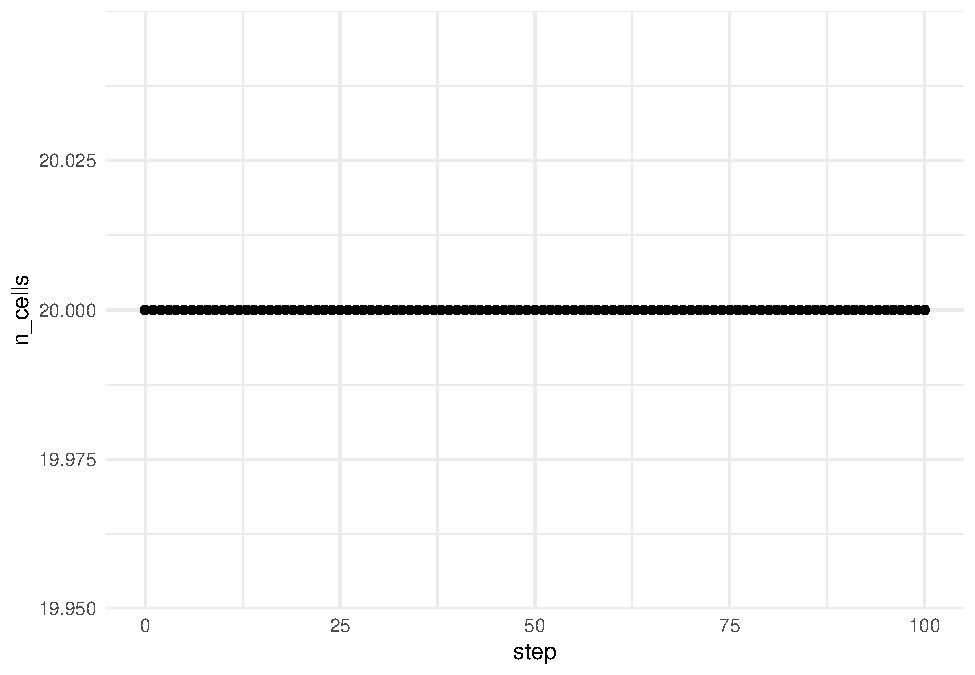
\includegraphics{lifesimulatoR-book_files/lifesimulatoR-book_files/figure-latex/protocell-plot-1.pdf}

This plot illustrates how the number of protocells changes as growth, leakage, and division interact.

\section{Understanding Growth}\label{understanding-growth}

Growth represents the accumulation of internal material.

In real systems, growth might result from:

\begin{itemize}
\tightlist
\item
  nutrient uptake,
\item
  chemical reactions,
\item
  energy harvesting,
\item
  molecular synthesis.
\end{itemize}

In the simulation, growth is represented by a simplified parameter.

Higher growth rates generally increase the likelihood of division.

\section{Understanding Leakage}\label{understanding-leakage}

No membrane is perfect.

Early protocells were probably highly permeable.

Leakage represents the loss of internal material to the surrounding environment.

Leakage creates a tension between:

\begin{itemize}
\tightlist
\item
  retaining useful molecules,
\item
  allowing exchange with the environment.
\end{itemize}

Too much leakage may prevent protocells from maintaining sufficient internal organization.

\section{Experiment: Exploring Leakage}\label{experiment-exploring-leakage}

\begin{Shaded}
\begin{Highlighting}[]
\NormalTok{low\_leakage }\OtherTok{\textless{}{-}} \FunctionTok{protocell\_simulation}\NormalTok{(}
  \AttributeTok{n\_cells =} \DecValTok{20}\NormalTok{,}
  \AttributeTok{steps =} \DecValTok{100}\NormalTok{,}
  \AttributeTok{growth\_rate =} \FloatTok{0.2}\NormalTok{,}
  \AttributeTok{division\_threshold =} \DecValTok{10}\NormalTok{,}
  \AttributeTok{leakage\_rate =} \FloatTok{0.01}\NormalTok{,}
  \AttributeTok{seed =} \DecValTok{123}
\NormalTok{)}

\NormalTok{high\_leakage }\OtherTok{\textless{}{-}} \FunctionTok{protocell\_simulation}\NormalTok{(}
  \AttributeTok{n\_cells =} \DecValTok{20}\NormalTok{,}
  \AttributeTok{steps =} \DecValTok{100}\NormalTok{,}
  \AttributeTok{growth\_rate =} \FloatTok{0.2}\NormalTok{,}
  \AttributeTok{division\_threshold =} \DecValTok{10}\NormalTok{,}
  \AttributeTok{leakage\_rate =} \FloatTok{0.15}\NormalTok{,}
  \AttributeTok{seed =} \DecValTok{123}
\NormalTok{)}

\FunctionTok{tail}\NormalTok{(low\_leakage)}
\end{Highlighting}
\end{Shaded}

\begin{verbatim}
## # A tibble: 6 x 4
##    step n_cells mean_abundance max_abundance
##   <int>   <int>          <dbl>         <dbl>
## 1    95      74           6.65          9.73
## 2    96      74           6.78          9.88
## 3    97      75           6.84          9.95
## 4    98      76           6.89          9.85
## 5    99      77           6.95         10.00
## 6   100      79           6.91          9.89
\end{verbatim}

\begin{Shaded}
\begin{Highlighting}[]
\FunctionTok{tail}\NormalTok{(high\_leakage)}
\end{Highlighting}
\end{Shaded}

\begin{verbatim}
## # A tibble: 6 x 4
##    step n_cells mean_abundance max_abundance
##   <int>   <int>          <dbl>         <dbl>
## 1    95      20           1.26          1.51
## 2    96      20           1.27          1.54
## 3    97      20           1.27          1.61
## 4    98      20           1.27          1.55
## 5    99      20           1.28          1.64
## 6   100      20           1.26          1.53
\end{verbatim}

Comparing these simulations illustrates how membrane properties can strongly influence protocell success.

\section{The Trade-Off Between Openness and Isolation}\label{the-trade-off-between-openness-and-isolation}

One of the most important challenges faced by protocells is balancing openness and isolation.

A completely closed compartment may:

\begin{itemize}
\tightlist
\item
  retain useful molecules,
\item
  prevent nutrient exchange.
\end{itemize}

A completely open compartment may:

\begin{itemize}
\tightlist
\item
  access environmental resources,
\item
  lose valuable contents.
\end{itemize}

Successful protocells likely occupied an intermediate position.

This trade-off remains important even in modern cells.

\section{Division and Reproduction}\label{division-and-reproduction}

When a protocell reaches a threshold size, it divides.

Division is important because it allows successful compartments to generate descendants.

Although protocell division is not identical to modern biological reproduction, it introduces a primitive form of population growth.

This creates opportunities for selection to act at the compartment level.

\section{Selection Among Protocells}\label{selection-among-protocells}

An intriguing possibility is that selection may have operated on protocells themselves.

Consider two protocells:

\begin{itemize}
\tightlist
\item
  one retains useful molecules effectively,
\item
  one loses useful molecules rapidly.
\end{itemize}

The first protocell may grow faster and divide more often.

Over time, populations may become enriched in more successful compartment types.

This idea introduces the possibility of evolution occurring simultaneously at multiple levels:

\begin{itemize}
\tightlist
\item
  molecular evolution,
\item
  network evolution,
\item
  protocell evolution.
\end{itemize}

\section{The Hypercycle and Cooperative Systems}\label{the-hypercycle-and-cooperative-systems}

Some origin-of-life researchers have proposed that compartments may help stabilize cooperative molecular systems.

Without compartments:

\begin{itemize}
\tightlist
\item
  selfish molecules may dominate,
\item
  cooperative systems may collapse.
\end{itemize}

With compartments:

\begin{itemize}
\tightlist
\item
  groups of cooperating molecules can remain together,
\item
  cooperative networks may become more stable.
\end{itemize}

This idea plays an important role in several theories of early evolution.

\section{Interpreting Simulation Results}\label{interpreting-simulation-results-1}

Several outcomes are possible.

\subsection{Increasing Protocell Numbers}\label{increasing-protocell-numbers}

May indicate:

\begin{itemize}
\tightlist
\item
  successful growth,
\item
  sufficient retention,
\item
  frequent division.
\end{itemize}

\subsection{Stable Populations}\label{stable-populations}

May indicate:

\begin{itemize}
\tightlist
\item
  balance between growth and leakage.
\end{itemize}

\subsection{Declining Populations}\label{declining-populations}

May indicate:

\begin{itemize}
\tightlist
\item
  excessive leakage,
\item
  insufficient growth,
\item
  inability to divide.
\end{itemize}

Different parameter combinations can produce very different population dynamics.

\section{Limitations of the Model}\label{limitations-of-the-model-2}

The protocell model in \texttt{lifesimulatoR} is intentionally simplified.

It does not include:

\begin{itemize}
\tightlist
\item
  membrane chemistry,
\item
  lipid synthesis,
\item
  osmotic effects,
\item
  nutrient transport,
\item
  internal reaction networks,
\item
  molecular composition,
\item
  environmental variability.
\end{itemize}

Its purpose is to illustrate the conceptual importance of compartmentalization rather than reproduce realistic protocell behavior.

\section{Connections to Other Chapters}\label{connections-to-other-chapters-1}

This chapter builds upon:

\begin{itemize}
\tightlist
\item
  prebiotic chemistry,
\item
  molecular evolution,
\item
  diversity and complexity.
\end{itemize}

It prepares the foundation for the next chapter on autocatalytic networks.

Together these chapters explore how molecules, information, networks, and compartments may have interacted during the emergence of life.

\section{Key Takeaways}\label{key-takeaways-2}

\begin{itemize}
\tightlist
\item
  Compartments may have been essential for the emergence of life.
\item
  Protocells provide a bridge between chemistry and biology.
\item
  Compartments concentrate molecules and facilitate interactions.
\item
  Leakage and growth create important evolutionary trade-offs.
\item
  Division introduces a primitive form of inheritance and reproduction.
\item
  Selection may operate on compartments as well as molecules.
\item
  Many origin-of-life theories view protocells as critical intermediates.
\item
  \texttt{lifesimulatoR} provides a simplified framework for exploring these ideas.
\end{itemize}

\section{Suggested Readings}\label{suggested-readings-2}

\begin{itemize}
\tightlist
\item
  Luisi, P. L. (2006). \emph{The Emergence of Life.}
\item
  Szostak, J. W., Bartel, D. P., \& Luisi, P. L. (2001). Synthesizing Life.
\item
  Deamer, D. (2019). \emph{Assembling Life.}
\item
  Morowitz, H. J. (1992). \emph{Beginnings of Cellular Life.}
\item
  Rasmussen, S. et al.~(2008). \emph{Protocells: Bridging Nonliving and Living Matter.}
\end{itemize}

\section{Reflection Questions}\label{reflection-questions-4}

\begin{enumerate}
\def\labelenumi{\arabic{enumi}.}
\tightlist
\item
  Why are compartments important for the emergence of life?
\item
  Can selection act on protocells themselves?
\item
  What advantages do compartments provide compared with open environments?
\item
  What trade-offs arise between membrane permeability and retention?
\item
  Could molecular evolution occur without compartments?
\item
  How might protocells and replicators have co-evolved?
\item
  What aspects of real membrane biology are missing from this model?
\item
  Could compartments emerge before information-bearing molecules?
\item
  Why might cooperation be easier inside compartments?
\item
  How might future simulations incorporate molecular contents and membrane chemistry?
\end{enumerate}

\chapter{Autocatalytic Networks}\label{autocatalytic-networks}

\section{Why Autocatalytic Networks Matter}\label{why-autocatalytic-networks-matter}

One of the central questions in origin-of-life research is how simple chemistry became capable of self-maintenance and evolution.

Many origin-of-life theories focus on replication. In these models, a molecule capable of copying itself is viewed as the starting point of evolution.

However, another possibility exists.

Instead of a single molecule reproducing itself, an entire network of molecules may collectively sustain its own production.

This idea forms the basis of autocatalytic network theory.

In this view:

\begin{quote}
Life may have begun not with a single replicator, but with a community of mutually supportive molecules.
\end{quote}

Autocatalytic networks provide one possible explanation for how organization emerged before the appearance of modern genes.

\section{What Is Catalysis?}\label{what-is-catalysis}

Catalysis occurs when one molecule increases the rate of a chemical reaction without being permanently consumed.

Catalysts are essential in modern biology.

Examples include:

\begin{itemize}
\tightlist
\item
  enzymes accelerating metabolic reactions,
\item
  ribozymes catalyzing RNA reactions,
\item
  mineral surfaces promoting chemical transformations.
\end{itemize}

Without catalysis, many biological reactions would proceed far too slowly to sustain life.

Catalysis therefore provides a mechanism by which chemical systems can become increasingly organized.

\section{What Is an Autocatalytic Network?}\label{what-is-an-autocatalytic-network}

An autocatalytic network is a collection of molecules in which members of the network help produce one another.

For example:

Molecule A helps produce Molecule B.

Molecule B helps produce Molecule C.

Molecule C helps produce Molecule A.

No single molecule is self-sufficient.

However, the network as a whole becomes self-reinforcing.

This creates an important shift in perspective:

\begin{quote}
The unit of organization becomes the network rather than the individual molecule.
\end{quote}

\section{Historical Background}\label{historical-background}

The concept of autocatalytic networks became particularly influential through the work of Stuart Kauffman.

Kauffman proposed that sufficiently complex chemical systems may naturally undergo a transition from disconnected reactions to self-sustaining networks.

This idea suggested a possible route to life's emergence that does not require a highly improbable self-replicating molecule appearing first.

Instead:

\begin{itemize}
\tightlist
\item
  diversity increases,
\item
  catalytic interactions accumulate,
\item
  networks become increasingly connected,
\item
  self-maintaining systems emerge.
\end{itemize}

This perspective remains an important alternative to purely gene-first theories.

\section{Network-First Versus Replication-First Models}\label{network-first-versus-replication-first-models}

Two broad approaches to the origin of life can be contrasted.

\subsection{Replication-First Models}\label{replication-first-models}

Focus on:

\begin{itemize}
\tightlist
\item
  informational molecules,
\item
  heredity,
\item
  mutation,
\item
  selection.
\end{itemize}

Examples:

\begin{itemize}
\tightlist
\item
  RNA World hypothesis
\item
  genetic-first scenarios
\end{itemize}

\subsection{Network-First Models}\label{network-first-models}

Focus on:

\begin{itemize}
\tightlist
\item
  chemical organization,
\item
  catalysis,
\item
  metabolic interactions,
\item
  collective self-maintenance.
\end{itemize}

Examples:

\begin{itemize}
\tightlist
\item
  autocatalytic set theory
\item
  metabolism-first theories
\end{itemize}

Many modern researchers suspect that both perspectives may capture important aspects of life's emergence.

\section{Emergence in Chemical Networks}\label{emergence-in-chemical-networks}

Autocatalytic networks provide an excellent example of emergence.

No individual molecule may possess life-like properties.

However, when many molecules interact:

\begin{itemize}
\tightlist
\item
  feedback loops appear,
\item
  self-maintenance emerges,
\item
  system-level organization develops.
\end{itemize}

The resulting behavior cannot always be predicted by examining molecules individually.

This illustrates one of the central themes of complexity science:

\begin{quote}
The whole can exhibit properties that are not obvious from the parts.
\end{quote}

\section{Conceptual Model}\label{conceptual-model-4}

In \texttt{lifesimulatoR}, an autocatalytic network is represented using:

\begin{itemize}
\tightlist
\item
  molecular types,
\item
  catalytic relationships,
\item
  abundance changes through time,
\item
  a catalysis matrix.
\end{itemize}

Although highly simplified, this framework captures the essential idea of mutual reinforcement.

\section{Creating an Autocatalytic Network}\label{creating-an-autocatalytic-network}

\begin{Shaded}
\begin{Highlighting}[]
\NormalTok{network }\OtherTok{\textless{}{-}} \FunctionTok{autocatalytic\_network}\NormalTok{(}
  \AttributeTok{n\_types =} \DecValTok{8}\NormalTok{,}
  \AttributeTok{steps =} \DecValTok{50}\NormalTok{,}
  \AttributeTok{catalysis\_probability =} \FloatTok{0.2}\NormalTok{,}
  \AttributeTok{seed =} \DecValTok{123}
\NormalTok{)}

\FunctionTok{names}\NormalTok{(network)}
\end{Highlighting}
\end{Shaded}

\begin{verbatim}
## [1] "time_series"      "catalysis_matrix"
\end{verbatim}

\begin{Shaded}
\begin{Highlighting}[]
\FunctionTok{head}\NormalTok{(network}\SpecialCharTok{$}\NormalTok{time\_series)}
\end{Highlighting}
\end{Shaded}

\begin{verbatim}
## # A tibble: 6 x 3
##    step molecule abundance
##   <int> <chr>        <dbl>
## 1     0 M1           0.833
## 2     0 M2           0.504
## 3     0 M3           0.829
## 4     0 M4           0.831
## 5     0 M5           0.815
## 6     0 M6           0.496
\end{verbatim}

The output contains both network structure and abundance dynamics.

\section{Understanding the Catalysis Matrix}\label{understanding-the-catalysis-matrix}

The catalysis matrix records which molecules catalyze the production of others.

\texttt{\{r\ autocatalytic-matrix\}\ id="autocatalytic-matrix"\ network\$catalysis\_matrix}

The matrix can be viewed as a map of catalytic interactions.

Each connection represents a potential pathway through which molecules influence one another.

\section{Visualizing Molecular Dynamics}\label{visualizing-molecular-dynamics}

We can examine the abundance of a particular molecular type.

\begin{Shaded}
\begin{Highlighting}[]
\NormalTok{m1 }\OtherTok{\textless{}{-}} \FunctionTok{subset}\NormalTok{(}
\NormalTok{  network}\SpecialCharTok{$}\NormalTok{time\_series,}
\NormalTok{  molecule }\SpecialCharTok{==} \StringTok{"M1"}
\NormalTok{)}

\FunctionTok{plot\_simulation}\NormalTok{(}
\NormalTok{  m1,}
  \AttributeTok{x =} \StringTok{"step"}\NormalTok{,}
  \AttributeTok{y =} \StringTok{"abundance"}
\NormalTok{)}
\end{Highlighting}
\end{Shaded}

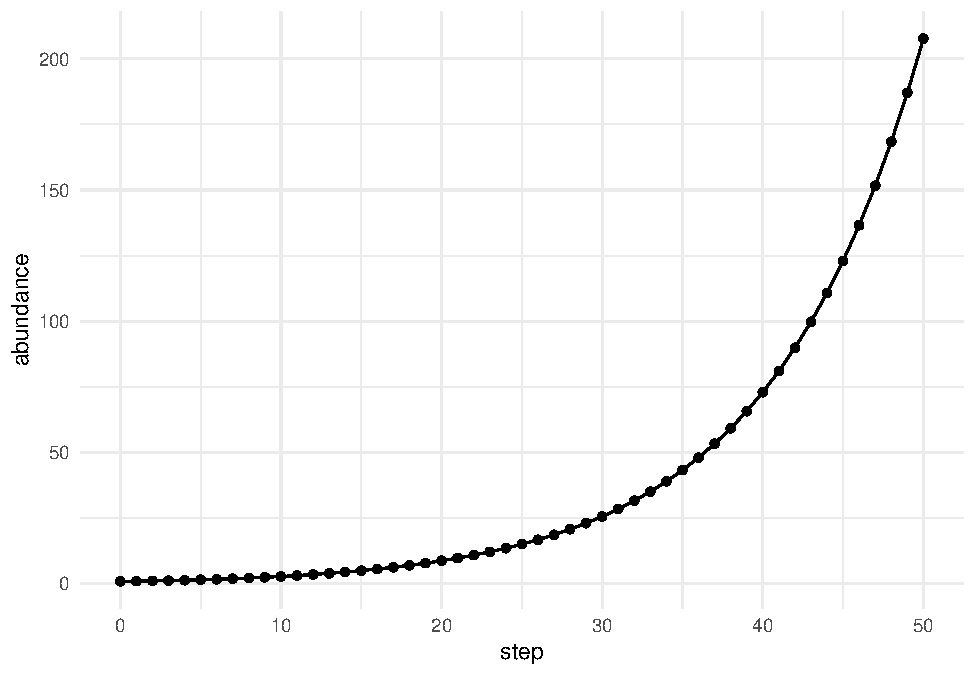
\includegraphics{lifesimulatoR-book_files/lifesimulatoR-book_files/figure-latex/autocatalytic-plot-1.pdf}

This plot shows how one molecule changes through time as it participates in the broader network.

\section{Feedback Loops}\label{feedback-loops}

One of the most important features of autocatalytic systems is the presence of feedback.

\subsection{Positive Feedback}\label{positive-feedback}

Positive feedback amplifies change.

Example:

A promotes B

B promotes C

C promotes A

Growth of one component reinforces the others.

\subsection{Negative Feedback}\label{negative-feedback}

Negative feedback stabilizes systems and prevents runaway growth.

Modern biological systems contain both positive and negative feedback loops.

Understanding feedback is essential for understanding living systems.

\section{Network Connectivity}\label{network-connectivity}

An important property of a network is connectivity.

Connectivity refers to how many interactions exist among components.

Low connectivity produces sparse networks.

High connectivity produces dense networks.

The level of connectivity strongly influences network behavior.

\section{Sparse Versus Dense Networks}\label{sparse-versus-dense-networks}

\begin{Shaded}
\begin{Highlighting}[]
\NormalTok{sparse\_network }\OtherTok{\textless{}{-}} \FunctionTok{autocatalytic\_network}\NormalTok{(}
  \AttributeTok{n\_types =} \DecValTok{8}\NormalTok{,}
  \AttributeTok{steps =} \DecValTok{50}\NormalTok{,}
  \AttributeTok{catalysis\_probability =} \FloatTok{0.05}\NormalTok{,}
  \AttributeTok{seed =} \DecValTok{123}
\NormalTok{)}

\NormalTok{dense\_network }\OtherTok{\textless{}{-}} \FunctionTok{autocatalytic\_network}\NormalTok{(}
  \AttributeTok{n\_types =} \DecValTok{8}\NormalTok{,}
  \AttributeTok{steps =} \DecValTok{50}\NormalTok{,}
  \AttributeTok{catalysis\_probability =} \FloatTok{0.4}\NormalTok{,}
  \AttributeTok{seed =} \DecValTok{123}
\NormalTok{)}

\FunctionTok{head}\NormalTok{(sparse\_network}\SpecialCharTok{$}\NormalTok{time\_series)}
\end{Highlighting}
\end{Shaded}

\begin{verbatim}
## # A tibble: 6 x 3
##    step molecule abundance
##   <int> <chr>        <dbl>
## 1     0 M1           0.833
## 2     0 M2           0.504
## 3     0 M3           0.829
## 4     0 M4           0.831
## 5     0 M5           0.815
## 6     0 M6           0.496
\end{verbatim}

\begin{Shaded}
\begin{Highlighting}[]
\FunctionTok{head}\NormalTok{(dense\_network}\SpecialCharTok{$}\NormalTok{time\_series)}
\end{Highlighting}
\end{Shaded}

\begin{verbatim}
## # A tibble: 6 x 3
##    step molecule abundance
##   <int> <chr>        <dbl>
## 1     0 M1           0.833
## 2     0 M2           0.504
## 3     0 M3           0.829
## 4     0 M4           0.831
## 5     0 M5           0.815
## 6     0 M6           0.496
\end{verbatim}

Dense networks are more likely to contain:

\begin{itemize}
\tightlist
\item
  feedback loops,
\item
  indirect interactions,
\item
  collective dynamics.
\end{itemize}

Sparse networks tend to be less interconnected.

\section{The Autocatalytic Threshold}\label{the-autocatalytic-threshold}

Kauffman proposed that sufficiently connected networks may experience a phase transition.

Below a critical threshold:

\begin{itemize}
\tightlist
\item
  reactions remain largely disconnected.
\end{itemize}

Above the threshold:

\begin{itemize}
\tightlist
\item
  self-sustaining networks become possible.
\end{itemize}

This idea is similar to phase transitions observed elsewhere in nature, such as:

\begin{itemize}
\tightlist
\item
  water freezing,
\item
  magnets becoming ordered,
\item
  percolation in physical systems.
\end{itemize}

The emergence of autocatalytic sets may represent a comparable transition in chemical organization.

\section{Autocatalytic Networks and Evolution}\label{autocatalytic-networks-and-evolution}

Autocatalytic networks raise an important question:

Can evolution occur before genetic replication?

Some researchers argue that network-level selection may occur when:

\begin{itemize}
\tightlist
\item
  certain networks persist longer,
\item
  certain networks utilize resources more efficiently,
\item
  certain networks generate more stable structures.
\end{itemize}

If so, evolution may have begun before modern genes existed.

\section{Networks Inside Protocells}\label{networks-inside-protocells}

Autocatalytic networks become even more interesting when combined with compartments.

A protocell can:

\begin{itemize}
\tightlist
\item
  retain catalytic molecules,
\item
  protect network components,
\item
  maintain higher concentrations,
\item
  enable network inheritance during division.
\end{itemize}

Many modern theories propose that life emerged through interactions among:

\begin{itemize}
\tightlist
\item
  molecular evolution,
\item
  autocatalytic networks,
\item
  protocells.
\end{itemize}

Rather than one appearing first, these systems may have co-evolved.

\section{Interpreting Simulation Results}\label{interpreting-simulation-results-2}

Several outcomes are possible.

\subsection{Stable Abundances}\label{stable-abundances}

May indicate:

\begin{itemize}
\tightlist
\item
  balanced network interactions,
\item
  stable catalytic relationships.
\end{itemize}

\subsection{Increasing Abundances}\label{increasing-abundances}

May indicate:

\begin{itemize}
\tightlist
\item
  strong positive feedback,
\item
  successful catalytic reinforcement.
\end{itemize}

\subsection{Large Fluctuations}\label{large-fluctuations}

May indicate:

\begin{itemize}
\tightlist
\item
  unstable network dynamics,
\item
  sensitivity to network structure.
\end{itemize}

\subsection{Collapse of Components}\label{collapse-of-components}

May indicate:

\begin{itemize}
\tightlist
\item
  insufficient support from the rest of the network.
\end{itemize}

Different network architectures can produce dramatically different outcomes.

\section{Limitations of the Model}\label{limitations-of-the-model-3}

The autocatalytic network model in \texttt{lifesimulatoR} is intentionally simplified.

It does not include:

\begin{itemize}
\tightlist
\item
  realistic reaction kinetics,
\item
  thermodynamic constraints,
\item
  energy requirements,
\item
  environmental variation,
\item
  molecular structure,
\item
  reaction mechanisms,
\item
  resource competition.
\end{itemize}

Its purpose is to illustrate the principles of network organization and emergence rather than reproduce real chemistry.

\section{Connections to Other Chapters}\label{connections-to-other-chapters-2}

This chapter integrates many ideas developed earlier.

Prebiotic chemistry provides molecular diversity.

Molecular evolution introduces information and selection.

Diversity creates opportunities for interaction.

Protocells create compartments.

Autocatalytic networks provide organization.

Together these components illustrate several of the major pathways proposed for the emergence of life.

\section{Key Takeaways}\label{key-takeaways-3}

\begin{itemize}
\tightlist
\item
  Autocatalytic networks consist of mutually reinforcing molecules.
\item
  Organization can emerge from interactions among many components.
\item
  Networks may provide an alternative to purely replication-first origin-of-life theories.
\item
  Feedback loops play a central role in network behavior.
\item
  Connectivity strongly influences network dynamics.
\item
  Self-sustaining systems may emerge above critical network thresholds.
\item
  Autocatalytic networks become especially powerful when combined with protocells.
\item
  \texttt{lifesimulatoR} provides a simplified framework for exploring these ideas.
\end{itemize}

\section{Suggested Readings}\label{suggested-readings-3}

\begin{itemize}
\tightlist
\item
  Kauffman, S. (1993). \emph{The Origins of Order.}
\item
  Dyson, F. (1985). \emph{Origins of Life.}
\item
  Hordijk, W., \& Steel, M. (2004). Detecting Autocatalytic Sets.
\item
  Smith, E., \& Morowitz, H. (2016). \emph{The Origin and Nature of Life on Earth.}
\item
  Walker, S. I. (2017). Origins of Life and Complexity.
\end{itemize}

\section{Reflection Questions}\label{reflection-questions-5}

\begin{enumerate}
\def\labelenumi{\arabic{enumi}.}
\tightlist
\item
  How does a network-first model differ from a replication-first model?
\item
  Can organization emerge without genetic information?
\item
  What role do feedback loops play in complex systems?
\item
  Why might connectivity be important for life's emergence?
\item
  Could autocatalytic networks evolve before genes existed?
\item
  How might protocells stabilize catalytic networks?
\item
  What limitations arise when modeling networks using simple abstractions?
\item
  Can complexity emerge without selection?
\item
  Are autocatalytic networks sufficient for life, or merely one component of it?
\item
  Could life's origin have required both networks and replicators simultaneously?
\end{enumerate}

\chapter{Comparing Origin-of-Life Frameworks}\label{comparing-origin-of-life-frameworks}

\section{Why This Chapter Matters}\label{why-this-chapter-matters}

The previous chapters introduced several major pieces of the origin-of-life puzzle:

\begin{itemize}
\tightlist
\item
  Prebiotic chemistry
\item
  Molecular evolution
\item
  Diversity and complexity
\item
  Protocells
\item
  Autocatalytic networks
\end{itemize}

Each topic explains something important, but none of them alone fully explains the origin of life.

This chapter brings these ideas together.

The goal is not to choose one theory as the final answer. Instead, the goal is to compare what each framework explains well, what it struggles to explain, and how multiple frameworks may fit together.

\section{The Central Problem}\label{the-central-problem}

Origin-of-life research asks how non-living chemistry became living biology.

This transition likely required several processes to become linked:

\begin{itemize}
\tightlist
\item
  Molecular building blocks had to form
\item
  Molecules had to interact
\item
  Some systems had to persist
\item
  Information had to be stored and transmitted
\item
  Variation had to appear
\item
  Selection had to act
\item
  Compartments had to organize chemical systems
\item
  Energy flow had to sustain reactions
\end{itemize}

Different theories emphasize different starting points.

\section{Major Origin-of-Life Frameworks}\label{major-origin-of-life-frameworks}

Origin-of-life theories often differ in what they treat as the first major breakthrough.

\begin{longtable}[]{@{}
  >{\raggedright\arraybackslash}p{(\columnwidth - 4\tabcolsep) * \real{0.3333}}
  >{\raggedright\arraybackslash}p{(\columnwidth - 4\tabcolsep) * \real{0.3333}}
  >{\raggedright\arraybackslash}p{(\columnwidth - 4\tabcolsep) * \real{0.3333}}@{}}
\toprule\noalign{}
\begin{minipage}[b]{\linewidth}\raggedright
Framework
\end{minipage} & \begin{minipage}[b]{\linewidth}\raggedright
Main Starting Point
\end{minipage} & \begin{minipage}[b]{\linewidth}\raggedright
Central Idea
\end{minipage} \\
\midrule\noalign{}
\endhead
\bottomrule\noalign{}
\endlastfoot
RNA World & Information-bearing molecules & RNA-like molecules stored information and catalyzed reactions \\
Metabolism First & Energy and reaction networks & Self-sustaining chemical cycles emerged before genes \\
Protocell First & Compartments & Cell-like boundaries organized chemistry \\
Autocatalytic Sets & Networks & Molecules collectively supported their own production \\
Hybrid Models & Integration & Life emerged from coupling among molecules, networks, compartments, and energy flow \\
\end{longtable}

These frameworks are sometimes presented as competitors, but they may also be complementary.

\section{RNA World}\label{rna-world}

The RNA World hypothesis proposes that early life may have been based on RNA-like molecules.

RNA is important because it can:

\begin{itemize}
\tightlist
\item
  Store information
\item
  Participate in catalysis
\item
  Be copied with variation
\item
  Support evolutionary dynamics
\end{itemize}

In this view, the origin of life begins with information-bearing molecules.

\section{What RNA World Explains Well}\label{what-rna-world-explains-well}

RNA World models help explain:

\begin{itemize}
\tightlist
\item
  Heredity
\item
  Mutation
\item
  Selection
\item
  Molecular evolution
\item
  The central role of RNA in modern biology
\end{itemize}

RNA still plays essential roles in living cells, including protein synthesis and regulation. This makes RNA a plausible relic of an earlier stage of life.

\section{What RNA World Struggles to Explain}\label{what-rna-world-struggles-to-explain}

RNA World models face several challenges:

\begin{itemize}
\tightlist
\item
  How did the first RNA-like molecules form?
\item
  How were nucleotides produced under prebiotic conditions?
\item
  How did long enough RNA molecules accumulate?
\item
  How did early replication become accurate enough?
\item
  How were RNA molecules protected from degradation?
\end{itemize}

The key difficulty is that RNA is chemically complex.

\section{RNA World in lifesimulatoR}\label{rna-world-in-lifesimulator}

\begin{Shaded}
\begin{Highlighting}[]
\NormalTok{rna\_like }\OtherTok{\textless{}{-}} \FunctionTok{simulate\_abiogenesis}\NormalTok{(}
  \AttributeTok{n\_molecules =} \DecValTok{100}\NormalTok{,}
  \AttributeTok{generations =} \DecValTok{100}\NormalTok{,}
  \AttributeTok{mutation\_rate =} \FloatTok{0.02}\NormalTok{,}
  \AttributeTok{selection\_strength =} \DecValTok{1}\NormalTok{,}
  \AttributeTok{seed =} \DecValTok{123}
\NormalTok{)}

\FunctionTok{head}\NormalTok{(rna\_like)}
\end{Highlighting}
\end{Shaded}

\begin{verbatim}
## # A tibble: 6 x 6
##   generation n_molecules mean_length mean_fitness diversity max_fitness
##        <int>       <int>       <dbl>        <dbl>     <int>       <dbl>
## 1          0         100        12.6         1.00       100        1.25
## 2          1         100        12.7         1.04        67        1.25
## 3          2         100        12.3         1.05        61        1.25
## 4          3         100        12.3         1.11        61        1.25
## 5          4         100        12.5         1.11        48        1.25
## 6          5         100        12.8         1.13        53        1.25
\end{verbatim}

\begin{Shaded}
\begin{Highlighting}[]
\FunctionTok{plot\_simulation}\NormalTok{(}
\NormalTok{  rna\_like,}
  \AttributeTok{x =} \StringTok{"generation"}\NormalTok{,}
  \AttributeTok{y =} \StringTok{"mean\_fitness"}
\NormalTok{)}
\end{Highlighting}
\end{Shaded}

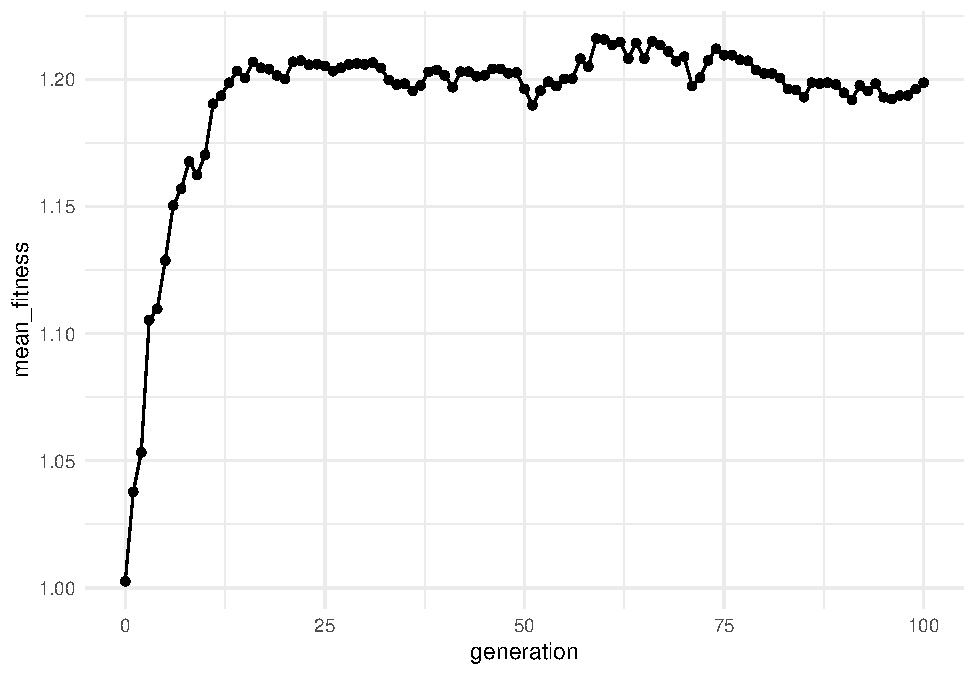
\includegraphics{lifesimulatoR-book_files/lifesimulatoR-book_files/figure-latex/rna-world-plot-1.pdf}

\section{Interpretation}\label{interpretation}

This simulation represents a simplified replication-first model.

If mean fitness increases, the model demonstrates how variation, mutation, replication, and selection can drive evolutionary change.

\section{Metabolism First}\label{metabolism-first}

Metabolism-first theories propose that life began with self-sustaining reaction networks rather than genetic molecules.

In this view, the earliest life-like systems may have been organized flows of matter and energy.

Instead of asking how the first genetic molecule formed, metabolism-first models ask:

\begin{quote}
How could chemistry organize itself into self-maintaining reaction cycles?
\end{quote}

\section{What Metabolism First Explains Well}\label{what-metabolism-first-explains-well}

Metabolism-first models help explain:

\begin{itemize}
\tightlist
\item
  Energy flow
\item
  Chemical self-organization
\item
  Reaction cycles
\item
  Geochemical continuity
\item
  Environmental gradients
\end{itemize}

These theories are frequently associated with hydrothermal vent environments.

\section{What Metabolism First Struggles to Explain}\label{what-metabolism-first-struggles-to-explain}

Metabolism-first models face several questions:

\begin{itemize}
\tightlist
\item
  How did reaction networks become heritable?
\item
  How did they evolve without genetic information?
\item
  How were successful networks preserved?
\item
  How did metabolism become linked to informational polymers?
\end{itemize}

The key difficulty is explaining how chemical organization became evolvable.

\section{Autocatalytic Set Theory}\label{autocatalytic-set-theory}

Autocatalytic set theory proposes that molecules formed networks in which members helped produce one another.

No single molecule needed to reproduce itself perfectly.

Instead, the network as a whole became self-supporting.

\section{What Autocatalytic Sets Explain Well}\label{what-autocatalytic-sets-explain-well}

Autocatalytic network models help explain:

\begin{itemize}
\tightlist
\item
  Collective organization
\item
  Self-maintenance
\item
  Feedback loops
\item
  Emergence
\item
  Network-level behavior
\end{itemize}

They demonstrate how system-level organization can arise from interactions among many components.

\section{What Autocatalytic Sets Struggle to Explain}\label{what-autocatalytic-sets-struggle-to-explain}

Autocatalytic set models face important questions:

\begin{itemize}
\tightlist
\item
  How is information stored?
\item
  How are successful networks inherited?
\item
  How does selection act on networks?
\item
  How do networks avoid collapse?
\item
  How do they become coupled to compartments?
\end{itemize}

The key difficulty is connecting network self-maintenance to heredity and evolution.

\section{Autocatalytic Networks in lifesimulatoR}\label{autocatalytic-networks-in-lifesimulator}

\begin{Shaded}
\begin{Highlighting}[]
\NormalTok{auto }\OtherTok{\textless{}{-}} \FunctionTok{autocatalytic\_network}\NormalTok{(}
  \AttributeTok{n\_types =} \DecValTok{8}\NormalTok{,}
  \AttributeTok{steps =} \DecValTok{50}\NormalTok{,}
  \AttributeTok{catalysis\_probability =} \FloatTok{0.2}\NormalTok{,}
  \AttributeTok{seed =} \DecValTok{123}
\NormalTok{)}

\FunctionTok{head}\NormalTok{(auto}\SpecialCharTok{$}\NormalTok{time\_series)}
\end{Highlighting}
\end{Shaded}

\begin{verbatim}
## # A tibble: 6 x 3
##    step molecule abundance
##   <int> <chr>        <dbl>
## 1     0 M1           0.833
## 2     0 M2           0.504
## 3     0 M3           0.829
## 4     0 M4           0.831
## 5     0 M5           0.815
## 6     0 M6           0.496
\end{verbatim}

\begin{Shaded}
\begin{Highlighting}[]
\NormalTok{auto}\SpecialCharTok{$}\NormalTok{catalysis\_matrix}
\end{Highlighting}
\end{Shaded}

\begin{verbatim}
##       [,1]  [,2]  [,3]  [,4]  [,5]  [,6]  [,7]  [,8]
## [1,] FALSE FALSE FALSE FALSE FALSE  TRUE FALSE  TRUE
## [2,] FALSE FALSE  TRUE FALSE FALSE FALSE FALSE FALSE
## [3,] FALSE FALSE FALSE FALSE  TRUE FALSE  TRUE FALSE
## [4,] FALSE FALSE FALSE FALSE FALSE FALSE FALSE FALSE
## [5,] FALSE FALSE FALSE FALSE FALSE  TRUE FALSE FALSE
## [6,]  TRUE FALSE FALSE  TRUE FALSE FALSE  TRUE  TRUE
## [7,] FALSE  TRUE FALSE FALSE FALSE FALSE FALSE FALSE
## [8,] FALSE FALSE FALSE FALSE FALSE FALSE FALSE FALSE
\end{verbatim}

\section{Interpretation}\label{interpretation-1}

This simulation illustrates how catalytic relationships can produce system-level dynamics.

The model does not simulate real reaction chemistry, but it helps explore how networks can become more important than individual molecules.

\section{Protocell First}\label{protocell-first}

Protocell-first theories emphasize the importance of compartments.

A protocell is a simplified cell-like structure that separates an internal chemical environment from the outside world.

Compartments may have helped early systems by:

\begin{itemize}
\tightlist
\item
  Concentrating molecules
\item
  Protecting fragile chemistry
\item
  Allowing repeated interactions
\item
  Supporting primitive inheritance
\item
  Creating units of selection
\end{itemize}

\section{What Protocell Models Explain Well}\label{what-protocell-models-explain-well}

Protocell models help explain:

\begin{itemize}
\tightlist
\item
  Individuality
\item
  Boundaries
\item
  Growth
\item
  Division
\item
  Group-level selection
\item
  The transition from chemistry to cell-like systems
\end{itemize}

Compartments are especially important because modern life is cellular.

\section{What Protocell Models Struggle to Explain}\label{what-protocell-models-struggle-to-explain}

Protocell-first models also face challenges:

\begin{itemize}
\tightlist
\item
  What molecules formed the first membranes?
\item
  How did protocells grow and divide reliably?
\item
  How were useful internal molecules retained?
\item
  How did protocells acquire metabolism or genetic systems?
\item
  How did protocell traits become heritable?
\end{itemize}

The key difficulty is explaining how compartments became linked to internal chemistry and information.

\section{Protocells in lifesimulatoR}\label{protocells-in-lifesimulator}

\begin{Shaded}
\begin{Highlighting}[]
\NormalTok{proto }\OtherTok{\textless{}{-}} \FunctionTok{protocell\_simulation}\NormalTok{(}
  \AttributeTok{n\_cells =} \DecValTok{20}\NormalTok{,}
  \AttributeTok{steps =} \DecValTok{100}\NormalTok{,}
  \AttributeTok{growth\_rate =} \FloatTok{0.2}\NormalTok{,}
  \AttributeTok{division\_threshold =} \DecValTok{10}\NormalTok{,}
  \AttributeTok{leakage\_rate =} \FloatTok{0.03}\NormalTok{,}
  \AttributeTok{seed =} \DecValTok{123}
\NormalTok{)}

\FunctionTok{head}\NormalTok{(proto)}
\end{Highlighting}
\end{Shaded}

\begin{verbatim}
## # A tibble: 6 x 4
##    step n_cells mean_abundance max_abundance
##   <int>   <int>          <dbl>         <dbl>
## 1     0      20           2.10          2.91
## 2     1      20           2.24          3.14
## 3     2      20           2.39          3.24
## 4     3      20           2.54          3.58
## 5     4      20           2.67          3.78
## 6     5      20           2.80          3.95
\end{verbatim}

\begin{Shaded}
\begin{Highlighting}[]
\FunctionTok{plot\_simulation}\NormalTok{(}
\NormalTok{  proto,}
  \AttributeTok{x =} \StringTok{"step"}\NormalTok{,}
  \AttributeTok{y =} \StringTok{"n\_cells"}
\NormalTok{)}
\end{Highlighting}
\end{Shaded}

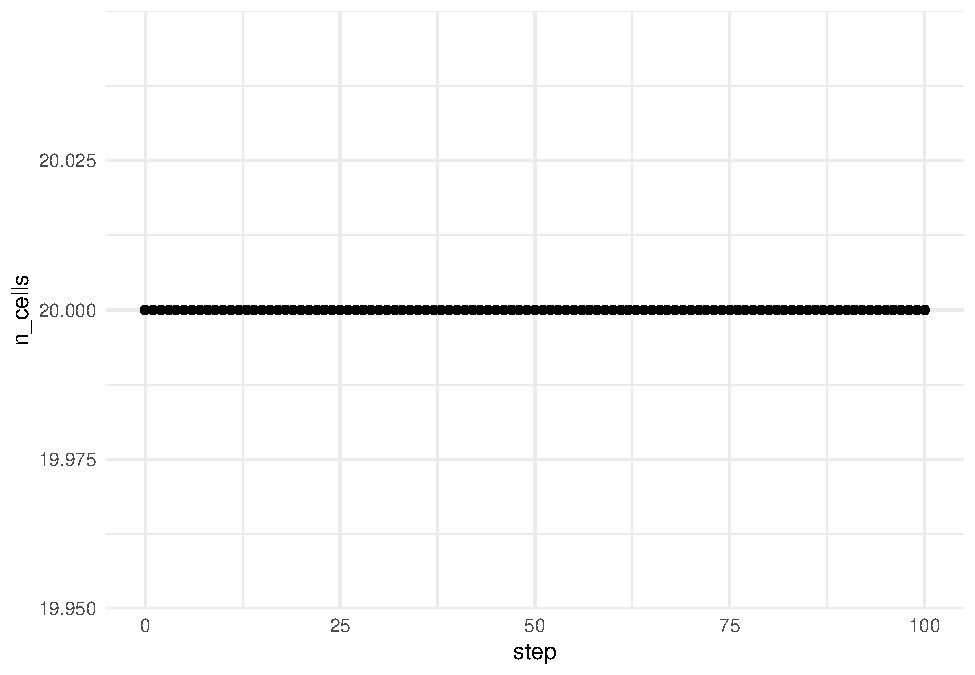
\includegraphics{lifesimulatoR-book_files/lifesimulatoR-book_files/figure-latex/compare-proto-plot-1.pdf}

\section{Interpretation}\label{interpretation-2}

This simulation shows how simple growth, leakage, and division rules can create protocell population dynamics.

\section{The Chicken-and-Egg Problem}\label{the-chicken-and-egg-problem}

A central challenge in origin-of-life research is the chicken-and-egg problem.

Which came first?

\begin{itemize}
\tightlist
\item
  Information?
\item
  Metabolism?
\item
  Compartments?
\item
  Networks?
\end{itemize}

Different theories answer differently.

\section{Possible Sequences}\label{possible-sequences}

\subsection{RNA World}\label{rna-world-1}

\begin{enumerate}
\def\labelenumi{\arabic{enumi}.}
\tightlist
\item
  Information
\item
  Replication
\item
  Evolution
\item
  Cells
\end{enumerate}

\subsection{Metabolism First}\label{metabolism-first-1}

\begin{enumerate}
\def\labelenumi{\arabic{enumi}.}
\tightlist
\item
  Energy flow
\item
  Reaction networks
\item
  Chemical self-maintenance
\item
  Information
\end{enumerate}

\subsection{Protocell First}\label{protocell-first-1}

\begin{enumerate}
\def\labelenumi{\arabic{enumi}.}
\tightlist
\item
  Compartments
\item
  Local chemistry
\item
  Growth and division
\item
  Internal evolution
\end{enumerate}

\subsection{Autocatalytic Sets}\label{autocatalytic-sets}

\begin{enumerate}
\def\labelenumi{\arabic{enumi}.}
\tightlist
\item
  Molecular diversity
\item
  Catalytic interactions
\item
  Network closure
\item
  Self-maintenance
\end{enumerate}

Hybrid models suggest that these processes may have developed together.

\section{Comparing Strengths and Limitations}\label{comparing-strengths-and-limitations}

\begin{longtable}[]{@{}
  >{\raggedright\arraybackslash}p{(\columnwidth - 4\tabcolsep) * \real{0.3333}}
  >{\raggedright\arraybackslash}p{(\columnwidth - 4\tabcolsep) * \real{0.3333}}
  >{\raggedright\arraybackslash}p{(\columnwidth - 4\tabcolsep) * \real{0.3333}}@{}}
\toprule\noalign{}
\begin{minipage}[b]{\linewidth}\raggedright
Framework
\end{minipage} & \begin{minipage}[b]{\linewidth}\raggedright
Explains Well
\end{minipage} & \begin{minipage}[b]{\linewidth}\raggedright
Struggles To Explain
\end{minipage} \\
\midrule\noalign{}
\endhead
\bottomrule\noalign{}
\endlastfoot
RNA World & Information, heredity, mutation, selection & Origin of first replicators \\
Metabolism First & Energy flow, reaction cycles & Heredity and evolvability \\
Protocell First & Boundaries, individuality & Origin of information systems \\
Autocatalytic Sets & Self-organization, feedback & Accurate inheritance \\
Hybrid Models & Integrates strengths & Harder to test experimentally \\
\end{longtable}

\section{Are These Theories Competitors?}\label{are-these-theories-competitors}

It is tempting to treat origin-of-life theories as mutually exclusive.

However, they may describe different parts of the same process.

For example:

\begin{itemize}
\tightlist
\item
  Prebiotic chemistry may have produced molecular diversity
\item
  Autocatalytic networks may have organized some molecules into self-maintaining systems
\item
  Protocells may have contained and protected these systems
\item
  RNA-like molecules may have introduced stronger heredity
\item
  Selection may have acted at both molecular and compartment levels
\end{itemize}

In this view, the origin of life was not a single event.

It was a sequence of transitions.

\section{Toward a Hybrid Model}\label{toward-a-hybrid-model}

A hybrid model may be the most realistic framework.

Such a model would include:

\begin{itemize}
\tightlist
\item
  Chemistry producing molecular diversity
\item
  Networks generating self-maintenance
\item
  Compartments creating individuality
\item
  Informational molecules enabling heredity
\item
  Energy flow sustaining reactions
\item
  Selection shaping populations
\end{itemize}

The central idea is:

\begin{quote}
Life may have emerged when chemistry, information, networks, compartments, and energy flow became coupled.
\end{quote}

\section{Conceptual Map}\label{conceptual-map}

\begin{Shaded}
\begin{Highlighting}[]
\NormalTok{Prebiotic chemistry}
\NormalTok{        ↓}
\NormalTok{Molecular diversity}
\NormalTok{        ↓}
\NormalTok{Autocatalytic interactions}
\NormalTok{        ↓}
\NormalTok{Compartmentalization}
\NormalTok{        ↓}
\NormalTok{Molecular evolution}
\NormalTok{        ↓}
\NormalTok{Coupled chemical systems}
\NormalTok{        ↓}
\NormalTok{Earliest life}
\end{Highlighting}
\end{Shaded}

\section{Package Comparison}\label{package-comparison}

The package allows users to explore simplified versions of several frameworks.

\subsection{Molecular Evolution}\label{molecular-evolution-1}

\begin{Shaded}
\begin{Highlighting}[]
\NormalTok{mol }\OtherTok{\textless{}{-}} \FunctionTok{simulate\_abiogenesis}\NormalTok{(}
  \AttributeTok{n\_molecules =} \DecValTok{100}\NormalTok{,}
  \AttributeTok{generations =} \DecValTok{100}\NormalTok{,}
  \AttributeTok{mutation\_rate =} \FloatTok{0.02}\NormalTok{,}
  \AttributeTok{selection\_strength =} \DecValTok{1}\NormalTok{,}
  \AttributeTok{seed =} \DecValTok{123}
\NormalTok{)}

\FunctionTok{tail}\NormalTok{(mol)}
\end{Highlighting}
\end{Shaded}

\begin{verbatim}
## # A tibble: 6 x 6
##   generation n_molecules mean_length mean_fitness diversity max_fitness
##        <int>       <int>       <dbl>        <dbl>     <int>       <dbl>
## 1         95         100        10.6         1.19        56        1.24
## 2         96         100        10.9         1.19        55        1.24
## 3         97         100        10.8         1.19        55        1.20
## 4         98         100        10.8         1.19        51        1.20
## 5         99         100        10.8         1.20        56        1.20
## 6        100         100        10.8         1.20        56        1.20
\end{verbatim}

\subsection{Protocells}\label{protocells}

\begin{Shaded}
\begin{Highlighting}[]
\NormalTok{proto }\OtherTok{\textless{}{-}} \FunctionTok{protocell\_simulation}\NormalTok{(}
  \AttributeTok{n\_cells =} \DecValTok{20}\NormalTok{,}
  \AttributeTok{steps =} \DecValTok{100}\NormalTok{,}
  \AttributeTok{seed =} \DecValTok{123}
\NormalTok{)}

\FunctionTok{tail}\NormalTok{(proto)}
\end{Highlighting}
\end{Shaded}

\begin{verbatim}
## # A tibble: 6 x 4
##    step n_cells mean_abundance max_abundance
##   <int>   <int>          <dbl>         <dbl>
## 1    95      20           6.84          7.44
## 2    96      20           6.85          7.41
## 3    97      20           6.87          7.43
## 4    98      20           6.89          7.48
## 5    99      20           6.91          7.56
## 6   100      20           6.90          7.49
\end{verbatim}

\subsection{Autocatalytic Networks}\label{autocatalytic-networks-1}

\begin{Shaded}
\begin{Highlighting}[]
\NormalTok{net }\OtherTok{\textless{}{-}} \FunctionTok{autocatalytic\_network}\NormalTok{(}
  \AttributeTok{n\_types =} \DecValTok{8}\NormalTok{,}
  \AttributeTok{steps =} \DecValTok{50}\NormalTok{,}
  \AttributeTok{catalysis\_probability =} \FloatTok{0.2}\NormalTok{,}
  \AttributeTok{seed =} \DecValTok{123}
\NormalTok{)}

\FunctionTok{tail}\NormalTok{(net}\SpecialCharTok{$}\NormalTok{time\_series)}
\end{Highlighting}
\end{Shaded}

\begin{verbatim}
## # A tibble: 6 x 3
##    step molecule abundance
##   <int> <chr>        <dbl>
## 1    50 M3            199.
## 2    50 M4            208.
## 3    50 M5            148.
## 4    50 M6            271.
## 5    50 M7            354.
## 6    50 M8            366.
\end{verbatim}

\section{What a Complete Model Would Need}\label{what-a-complete-model-would-need}

A more complete origin-of-life simulation would include:

\begin{itemize}
\tightlist
\item
  Realistic prebiotic chemistry
\item
  Energy sources and sinks
\item
  Molecular degradation
\item
  Catalytic reaction networks
\item
  Compartments
\item
  Transport across boundaries
\item
  Heredity
\item
  Mutation
\item
  Selection
\item
  Environmental change
\item
  Spatial structure
\end{itemize}

Such a model would be vastly more complex than the current educational simulations.

\section{Open Questions in Origin-of-Life Research}\label{open-questions-in-origin-of-life-research}

Despite decades of research, the origin of life remains one of science's greatest unsolved problems. Significant progress has been made, but many fundamental questions remain open.

\subsection{What Is Life?}\label{what-is-life}

A surprisingly difficult question is:

\begin{quote}
What exactly do we mean by life?
\end{quote}

Scientists generally agree that living systems exhibit characteristics such as:

\begin{itemize}
\tightlist
\item
  organization,
\item
  metabolism,
\item
  reproduction,
\item
  evolution,
\item
  information storage,
\item
  adaptation.
\end{itemize}

However, there is no universally accepted definition.

For example:

\begin{itemize}
\tightlist
\item
  Are viruses alive?
\item
  Could self-maintaining chemical systems be considered alive?
\item
  Is evolution required before a system can be called living?
\end{itemize}

Understanding the origin of life requires understanding what life itself actually is.

\subsection{How Did Information First Emerge?}\label{how-did-information-first-emerge}

Modern life depends on information stored in DNA and RNA.

Important questions include:

\begin{itemize}
\tightlist
\item
  Did RNA emerge first?
\item
  Were there earlier information systems?
\item
  How did molecular information become heritable?
\item
  How did accurate replication arise?
\end{itemize}

Information is central to biology, but its earliest origins remain uncertain.

\subsection{How Did Metabolism Begin?}\label{how-did-metabolism-begin}

Living systems continuously process energy and matter.

Open questions include:

\begin{itemize}
\tightlist
\item
  How did the first reaction networks arise?
\item
  Could metabolism emerge spontaneously?
\item
  What role did hydrothermal vents play?
\item
  How did energy flow become organized?
\end{itemize}

The emergence of metabolism remains one of the major challenges for origin-of-life theories.

\subsection{How Did Compartments Arise?}\label{how-did-compartments-arise}

Cells depend on membranes and compartments.

Researchers continue to investigate:

\begin{itemize}
\tightlist
\item
  What molecules formed the first membranes?
\item
  How stable were early protocells?
\item
  How did compartments interact with molecular evolution?
\item
  How did primitive cells become increasingly complex?
\end{itemize}

Compartmentalization may have been essential for transforming chemistry into biology.

\subsection{Was the Origin of Life Inevitable?}\label{was-the-origin-of-life-inevitable}

One of the most profound questions is whether life is common or rare.

Possible viewpoints include:

\begin{itemize}
\tightlist
\item
  Life emerges whenever suitable conditions exist.
\item
  Life is extremely unlikely and rare.
\item
  Multiple pathways can lead to life.
\item
  Life may emerge repeatedly under different chemical conditions.
\end{itemize}

At present, we do not know which possibility is correct.

\subsection{Is Life Common in the Universe?}\label{is-life-common-in-the-universe}

The search for life beyond Earth is closely connected to origin-of-life research.

Questions include:

\begin{itemize}
\tightlist
\item
  Did life emerge independently elsewhere?
\item
  What environments are most promising?
\item
  Should we expect life to resemble Earth life?
\item
  Could completely different forms of life exist?
\end{itemize}

Astrobiology continues to expand our understanding of these possibilities.

\section{Future Directions}\label{future-directions}

Origin-of-life research is advancing rapidly through new experiments, computational models, and interdisciplinary collaboration.

Several areas are likely to play major roles in future discoveries.

\subsection{Experimental Advances}\label{experimental-advances}

Researchers are actively exploring:

\begin{itemize}
\tightlist
\item
  Prebiotic synthesis pathways
\item
  Synthetic protocells
\item
  Artificial evolution experiments
\item
  RNA catalysis
\item
  Self-assembling chemical systems
\item
  Laboratory models of early Earth environments
\end{itemize}

These studies help constrain what may have been possible on the early Earth.

\subsection{Computational Advances}\label{computational-advances}

Computer simulations are becoming increasingly important.

Future models may include:

\begin{itemize}
\tightlist
\item
  Realistic reaction chemistry
\item
  Molecular folding
\item
  Environmental variability
\item
  Energy flow
\item
  Multi-level selection
\item
  Spatial structure
\item
  Network evolution
\item
  Coupled protocell-network systems
\end{itemize}

Computational models allow researchers to explore scenarios that are difficult to study experimentally.

\subsection{Future Directions for lifesimulatoR}\label{future-directions-for-lifesimulator}

The current package focuses on educational models. Future versions could incorporate more advanced concepts, including:

\begin{itemize}
\tightlist
\item
  RNA World simulations
\item
  Metabolism-first models
\item
  Hydrothermal vent environments
\item
  Wet-dry cycling chemistry
\item
  Lipid vesicle formation
\item
  Multi-level selection
\item
  Spatial simulations
\item
  Energy-gradient environments
\item
  Reaction-diffusion systems
\item
  Information-theoretic complexity metrics
\item
  Evolution of protocells
\item
  Coupled network-compartment simulations
\item
  Interactive Shiny applications
\item
  Animated educational visualizations
\end{itemize}

These additions would allow users to explore a broader range of origin-of-life hypotheses.

\section{Final Reflections}\label{final-reflections}

The origin of life remains one of the deepest scientific mysteries.

No single theory currently explains how non-living matter became living systems. Instead, researchers continue to investigate how molecular information, reaction networks, compartmentalization, and energy flow may have combined to produce the first life-like systems.

The purpose of this book has not been to provide a final answer. Rather, it has been to introduce the major ideas, theories, models, and questions that shape modern origin-of-life research.

Through the simplified simulations provided by \texttt{lifesimulatoR}, readers can explore these concepts directly and develop intuition about how complex biological systems may emerge from simpler beginnings.

The story of life's origins is still being written. Future discoveries may confirm existing theories, reveal entirely new mechanisms, or show that several frameworks must be combined to explain how life first emerged.

Perhaps the most exciting aspect of origin-of-life research is that some of the most important discoveries may still lie ahead.

\section{Key Takeaways}\label{key-takeaways-4}

\begin{itemize}
\tightlist
\item
  Origin-of-life theories emphasize different starting points.
\item
  RNA World focuses on information and heredity.
\item
  Metabolism First focuses on energy flow and reaction cycles.
\item
  Protocell First focuses on compartments and individuality.
\item
  Autocatalytic Set Theory focuses on network self-maintenance.
\item
  Hybrid models combine these ideas.
\item
  Theories may be complementary rather than mutually exclusive.
\item
  A complete theory likely requires chemistry, information, networks, compartments, and energy flow.
\item
  \texttt{lifesimulatoR} provides simplified models for exploring these frameworks.
\end{itemize}

\section{Suggested Readings}\label{suggested-readings-4}

\begin{itemize}
\tightlist
\item
  Gilbert, W. (1986). \emph{The RNA World}
\item
  Kauffman, S. (1993). \emph{The Origins of Order}
\item
  Deamer, D. (2019). \emph{Assembling Life}
\item
  Szostak, J. W., Bartel, D. P., \& Luisi, P. L. (2001). \emph{Synthesizing Life}
\item
  Smith, E., \& Morowitz, H. J. (2016). \emph{The Origin and Nature of Life on Earth}
\item
  Walker, S. I. (2017). \emph{Origins of Life and Complexity}
\end{itemize}

\section{Reflection Questions}\label{reflection-questions-6}

\begin{enumerate}
\def\labelenumi{\arabic{enumi}.}
\tightlist
\item
  Which framework seems most convincing?
\item
  Are these theories competitors or complementary explanations?
\item
  What does each framework explain particularly well?
\item
  What does each framework fail to explain?
\item
  Could life have emerged through several interacting processes rather than one dominant mechanism?
\item
  Which process seems most fundamental: information, metabolism, compartments, or networks?
\item
  What would be needed to build a more complete simulation?
\item
  How could \texttt{lifesimulatoR} be expanded to better compare these hypotheses?
\item
  Does a hybrid model make the origin of life easier or harder to explain?
\item
  What would count as strong evidence for one framework over another?
\end{enumerate}

\chapter{Appendix A: Package Function Reference}\label{appendix-a-package-function-reference}

\section{Purpose of This Appendix}\label{purpose-of-this-appendix}

This appendix serves as a comprehensive reference guide to the functions available in \texttt{lifesimulatoR}.

Throughout this book, we explored several major ideas in origin-of-life research, including:

\begin{itemize}
\tightlist
\item
  Prebiotic chemistry
\item
  Molecular evolution
\item
  Mutation and selection
\item
  Diversity and complexity
\item
  Protocells and compartmentalization
\item
  Autocatalytic networks
\item
  Competing origin-of-life frameworks
\end{itemize}

The goal of this appendix is to bring together all package functions in a single location and explain how they fit into the broader conceptual framework of the package.

The package is designed to support teaching, learning, science communication, and exploratory research through simplified computational models inspired by origin-of-life science.

\section{How the Package is Organized}\label{how-the-package-is-organized}

The package follows a simple conceptual workflow:

\begin{enumerate}
\def\labelenumi{\arabic{enumi}.}
\tightlist
\item
  Create molecular populations.
\item
  Measure molecular properties.
\item
  Replicate molecules.
\item
  Introduce mutation.
\item
  Apply selection.
\item
  Simulate evolutionary dynamics.
\item
  Measure diversity and complexity.
\item
  Explore alternative origin-of-life models.
\item
  Visualize results.
\end{enumerate}

These functions are intentionally simple so that the underlying scientific concepts remain transparent and easy to understand.

\section{A Typical Workflow}\label{a-typical-workflow}

A complete molecular evolution workflow might look like:

\begin{Shaded}
\begin{Highlighting}[]
\NormalTok{pool }\OtherTok{\textless{}{-}} \FunctionTok{create\_prebiotic\_pool}\NormalTok{()}

\NormalTok{fitness }\OtherTok{\textless{}{-}} \FunctionTok{molecule\_fitness}\NormalTok{(pool)}

\NormalTok{next\_generation }\OtherTok{\textless{}{-}} \FunctionTok{evolve\_generation}\NormalTok{(pool)}

\NormalTok{simulation }\OtherTok{\textless{}{-}} \FunctionTok{simulate\_abiogenesis}\NormalTok{()}

\FunctionTok{plot\_simulation}\NormalTok{(simulation)}
\end{Highlighting}
\end{Shaded}

This workflow represents a simplified progression from molecular diversity to evolutionary change.

\section{Package Workflow Diagram}\label{package-workflow-diagram}

\begin{Shaded}
\begin{Highlighting}[]
\NormalTok{Create molecules}
\NormalTok{        ↓}
\NormalTok{Measure properties}
\NormalTok{        ↓}
\NormalTok{Replicate}
\NormalTok{        ↓}
\NormalTok{Mutate}
\NormalTok{        ↓}
\NormalTok{Select}
\NormalTok{        ↓}
\NormalTok{Simulate evolution}
\NormalTok{        ↓}
\NormalTok{Analyze results}
\NormalTok{        ↓}
\NormalTok{Visualize outcomes}
\end{Highlighting}
\end{Shaded}

Alternative workflows explore protocells and autocatalytic networks independently of molecular evolution.

\section{Molecular Evolution Functions}\label{molecular-evolution-functions}

These functions support the molecular evolution framework discussed throughout the book.

\subsection{create\_prebiotic\_pool()}\label{create_prebiotic_pool}

Creates an initial population of symbolic molecules.

Purpose:

\begin{itemize}
\tightlist
\item
  Generate molecular diversity
\item
  Create starting populations
\item
  Explore prebiotic chemical space
\end{itemize}

Example:

\begin{Shaded}
\begin{Highlighting}[]
\NormalTok{pool }\OtherTok{\textless{}{-}} \FunctionTok{create\_prebiotic\_pool}\NormalTok{(}
  \AttributeTok{n\_molecules =} \DecValTok{100}\NormalTok{,}
  \AttributeTok{min\_length =} \DecValTok{5}\NormalTok{,}
  \AttributeTok{max\_length =} \DecValTok{20}
\NormalTok{)}
\end{Highlighting}
\end{Shaded}

Key concepts:

\begin{itemize}
\tightlist
\item
  Prebiotic chemistry
\item
  Molecular diversity
\item
  Chemical space exploration
\end{itemize}

\subsection{molecule\_fitness()}\label{molecule_fitness}

Assigns simplified fitness values to symbolic molecules.

Purpose:

\begin{itemize}
\tightlist
\item
  Model differential success
\item
  Support selection
\item
  Explore evolutionary dynamics
\end{itemize}

Example:

\begin{Shaded}
\begin{Highlighting}[]
\NormalTok{fitness }\OtherTok{\textless{}{-}} \FunctionTok{molecule\_fitness}\NormalTok{(pool)}
\end{Highlighting}
\end{Shaded}

Key concepts:

\begin{itemize}
\tightlist
\item
  Selection
\item
  Differential success
\item
  Evolutionary potential
\end{itemize}

\subsection{replicate\_molecules()}\label{replicate_molecules}

Generates offspring molecules according to fitness and selection.

Purpose:

\begin{itemize}
\tightlist
\item
  Simulate heredity
\item
  Create new generations
\item
  Explore selection effects
\end{itemize}

Example:

\begin{Shaded}
\begin{Highlighting}[]
\NormalTok{offspring }\OtherTok{\textless{}{-}} \FunctionTok{replicate\_molecules}\NormalTok{(pool)}
\end{Highlighting}
\end{Shaded}

Key concepts:

\begin{itemize}
\tightlist
\item
  Replication
\item
  Heredity
\item
  Population growth
\end{itemize}

\subsection{mutate\_sequence()}\label{mutate_sequence}

Mutates a single molecular sequence.

Purpose:

\begin{itemize}
\tightlist
\item
  Introduce novelty
\item
  Explore mutation effects
\item
  Demonstrate sequence variation
\end{itemize}

Example:

\begin{Shaded}
\begin{Highlighting}[]
\FunctionTok{mutate\_sequence}\NormalTok{(}
  \AttributeTok{sequence =} \StringTok{"AUGCAUGC"}\NormalTok{,}
  \AttributeTok{mutation\_rate =} \FloatTok{0.02}\NormalTok{,}
  \AttributeTok{alphabet =} \FunctionTok{c}\NormalTok{(}\StringTok{"A"}\NormalTok{, }\StringTok{"U"}\NormalTok{, }\StringTok{"G"}\NormalTok{, }\StringTok{"C"}\NormalTok{)}
\NormalTok{)}
\end{Highlighting}
\end{Shaded}

Key concepts:

\begin{itemize}
\tightlist
\item
  Mutation
\item
  Novelty
\item
  Sequence variation
\end{itemize}

\subsection{mutate\_population()}\label{mutate_population}

Applies mutation across an entire molecular population.

Purpose:

\begin{itemize}
\tightlist
\item
  Generate population-level variation
\item
  Support evolutionary simulations
\end{itemize}

Example:

\begin{Shaded}
\begin{Highlighting}[]
\FunctionTok{mutate\_population}\NormalTok{(}
  \AttributeTok{molecules =}\NormalTok{ pool,}
  \AttributeTok{mutation\_rate =} \FloatTok{0.02}
\NormalTok{)}
\end{Highlighting}
\end{Shaded}

Key concepts:

\begin{itemize}
\tightlist
\item
  Population-level variation
\item
  Evolutionary exploration
\end{itemize}

\subsection{evolve\_generation()}\label{evolve_generation}

Combines mutation, replication, and selection into a single evolutionary step.

Purpose:

\begin{itemize}
\tightlist
\item
  Model one generation of evolution
\item
  Combine mutation and selection
\item
  Produce the next generation
\end{itemize}

Example:

\begin{Shaded}
\begin{Highlighting}[]
\NormalTok{next\_generation }\OtherTok{\textless{}{-}} \FunctionTok{evolve\_generation}\NormalTok{(pool)}
\end{Highlighting}
\end{Shaded}

Key concepts:

\begin{itemize}
\tightlist
\item
  Evolutionary dynamics
\item
  Selection
\item
  Adaptation
\end{itemize}

\subsection{simulate\_abiogenesis()}\label{simulate_abiogenesis}

Runs a complete molecular evolution simulation over many generations.

Purpose:

\begin{itemize}
\tightlist
\item
  Explore evolutionary trajectories
\item
  Study mutation-selection dynamics
\item
  Simulate simplified origin-of-life scenarios
\end{itemize}

Example:

\begin{Shaded}
\begin{Highlighting}[]
\NormalTok{sim }\OtherTok{\textless{}{-}} \FunctionTok{simulate\_abiogenesis}\NormalTok{(}
  \AttributeTok{n\_molecules =} \DecValTok{100}\NormalTok{,}
  \AttributeTok{generations =} \DecValTok{200}
\NormalTok{)}
\end{Highlighting}
\end{Shaded}

Key concepts:

\begin{itemize}
\tightlist
\item
  Evolutionary trajectories
\item
  Population change through time
\item
  Origin-of-life modeling
\end{itemize}

\section{Diversity and Complexity Functions}\label{diversity-and-complexity-functions}

These functions help quantify variation and organization within molecular populations.

\subsection{summarize\_molecules()}\label{summarize_molecules}

Generates summary statistics for a molecular population.

Purpose:

\begin{itemize}
\tightlist
\item
  Summarize population properties
\item
  Monitor evolutionary change
\item
  Track simulation outcomes
\end{itemize}

Example:

\begin{Shaded}
\begin{Highlighting}[]
\FunctionTok{summarize\_molecules}\NormalTok{(pool)}
\end{Highlighting}
\end{Shaded}

Typical outputs include:

\begin{itemize}
\tightlist
\item
  Population size
\item
  Average sequence length
\item
  Diversity
\item
  Mean fitness
\item
  Maximum fitness
\end{itemize}

\subsection{shannon\_entropy()}\label{shannon_entropy}

Calculates Shannon entropy from abundance counts.

Purpose:

\begin{itemize}
\tightlist
\item
  Measure diversity
\item
  Explore information theory concepts
\item
  Compare molecular populations
\end{itemize}

Example:

\begin{Shaded}
\begin{Highlighting}[]
\NormalTok{counts }\OtherTok{\textless{}{-}} \FunctionTok{c}\NormalTok{(}\DecValTok{10}\NormalTok{, }\DecValTok{5}\NormalTok{, }\DecValTok{1}\NormalTok{)}

\FunctionTok{shannon\_entropy}\NormalTok{(counts)}
\end{Highlighting}
\end{Shaded}

Key concepts:

\begin{itemize}
\tightlist
\item
  Information theory
\item
  Diversity
\item
  Uncertainty
\item
  Complexity
\end{itemize}

\section{Visualization Functions}\label{visualization-functions}

Visualization helps reveal patterns that are difficult to see in raw numerical output.

\subsection{plot\_simulation()}\label{plot_simulation}

Creates plots from simulation outputs.

Purpose:

\begin{itemize}
\tightlist
\item
  Visualize evolutionary change
\item
  Explore diversity trends
\item
  Analyze protocell and network dynamics
\end{itemize}

Example:

\begin{Shaded}
\begin{Highlighting}[]
\FunctionTok{plot\_simulation}\NormalTok{(}
\NormalTok{  sim,}
  \AttributeTok{x =} \StringTok{"generation"}\NormalTok{,}
  \AttributeTok{y =} \StringTok{"mean\_fitness"}
\NormalTok{)}
\end{Highlighting}
\end{Shaded}

Common applications include:

\begin{itemize}
\tightlist
\item
  Fitness through time
\item
  Diversity through time
\item
  Population growth
\item
  Protocell dynamics
\item
  Network abundance trajectories
\end{itemize}

\section{Alternative Origin-of-Life Models}\label{alternative-origin-of-life-models}

These functions explore major alternatives and complements to replication-first models.

\subsection{protocell\_simulation()}\label{protocell_simulation}

Simulates protocell growth, leakage, and division.

Purpose:

\begin{itemize}
\tightlist
\item
  Explore compartmentalization
\item
  Investigate protocell dynamics
\item
  Study population growth
\end{itemize}

Example:

\begin{Shaded}
\begin{Highlighting}[]
\NormalTok{cells }\OtherTok{\textless{}{-}} \FunctionTok{protocell\_simulation}\NormalTok{(}
  \AttributeTok{n\_cells =} \DecValTok{20}\NormalTok{,}
  \AttributeTok{steps =} \DecValTok{100}
\NormalTok{)}
\end{Highlighting}
\end{Shaded}

Key concepts:

\begin{itemize}
\tightlist
\item
  Compartments
\item
  Growth
\item
  Division
\item
  Protocell evolution
\end{itemize}

Related chapter:

\begin{itemize}
\tightlist
\item
  Protocells and Compartmentalization
\end{itemize}

\subsection{autocatalytic\_network()}\label{autocatalytic_network}

Simulates catalytic network interactions.

Purpose:

\begin{itemize}
\tightlist
\item
  Explore self-maintaining systems
\item
  Study emergence
\item
  Investigate network organization
\end{itemize}

Example:

\begin{Shaded}
\begin{Highlighting}[]
\NormalTok{network }\OtherTok{\textless{}{-}} \FunctionTok{autocatalytic\_network}\NormalTok{(}
  \AttributeTok{n\_types =} \DecValTok{8}\NormalTok{,}
  \AttributeTok{steps =} \DecValTok{50}
\NormalTok{)}
\end{Highlighting}
\end{Shaded}

Key concepts:

\begin{itemize}
\tightlist
\item
  Catalysis
\item
  Feedback loops
\item
  Emergence
\item
  Network self-maintenance
\end{itemize}

Related chapter:

\begin{itemize}
\tightlist
\item
  Autocatalytic Networks
\end{itemize}

\section{Function Relationship Map}\label{function-relationship-map}

The following diagram summarizes how the major functions relate to one another.

\begin{Shaded}
\begin{Highlighting}[]
\NormalTok{create\_prebiotic\_pool()}
\NormalTok{            │}
\NormalTok{            ▼}
\NormalTok{   molecule\_fitness()}
\NormalTok{            │}
\NormalTok{            ▼}
\NormalTok{ replicate\_molecules()}
\NormalTok{            │}
\NormalTok{            ▼}
\NormalTok{  mutate\_population()}
\NormalTok{            │}
\NormalTok{            ▼}
\NormalTok{  evolve\_generation()}
\NormalTok{            │}
\NormalTok{            ▼}
\NormalTok{ simulate\_abiogenesis()}
\NormalTok{            │}
\NormalTok{            ▼}
\NormalTok{ summarize\_molecules()}
\NormalTok{            │}
\NormalTok{            ▼}
\NormalTok{   shannon\_entropy()}
\NormalTok{            │}
\NormalTok{            ▼}
\NormalTok{   plot\_simulation()}
\end{Highlighting}
\end{Shaded}

Alternative pathways:

\begin{Shaded}
\begin{Highlighting}[]
\NormalTok{protocell\_simulation()}

\NormalTok{autocatalytic\_network()}
\end{Highlighting}
\end{Shaded}

These models can be explored independently or conceptually linked to molecular evolution scenarios.

\section{Accessing Documentation}\label{accessing-documentation}

Every exported function includes documentation.

Useful commands include:

\begin{Shaded}
\begin{Highlighting}[]
\FunctionTok{help}\NormalTok{(}\AttributeTok{package =} \StringTok{"lifesimulatoR"}\NormalTok{)}

\NormalTok{?create\_prebiotic\_pool}
\NormalTok{?molecule\_fitness}
\NormalTok{?replicate\_molecules}
\NormalTok{?mutate\_sequence}
\NormalTok{?mutate\_population}
\NormalTok{?evolve\_generation}
\NormalTok{?simulate\_abiogenesis}
\NormalTok{?summarize\_molecules}
\NormalTok{?shannon\_entropy}
\NormalTok{?protocell\_simulation}
\NormalTok{?autocatalytic\_network}
\NormalTok{?plot\_simulation}

\FunctionTok{browseVignettes}\NormalTok{(}\StringTok{"lifesimulatoR"}\NormalTok{)}
\end{Highlighting}
\end{Shaded}

\section{Current Scope of the Package}\label{current-scope-of-the-package}

The package currently supports:

\begin{itemize}
\tightlist
\item
  Symbolic molecular evolution
\item
  Mutation and selection
\item
  Diversity measurement
\item
  Protocell simulations
\item
  Autocatalytic networks
\item
  Educational visualization
\end{itemize}

The models are intentionally simplified and should be viewed as educational tools rather than chemically realistic reconstructions of abiogenesis.

\section{Future Development}\label{future-development}

Potential future modules include:

\begin{itemize}
\tightlist
\item
  RNA World simulations
\item
  Metabolism-first models
\item
  Hydrothermal vent environments
\item
  Wet-dry cycling chemistry
\item
  Mineral surface catalysis
\item
  Energy-gradient simulations
\item
  Lipid vesicle formation
\item
  Multi-level selection
\item
  Spatial simulations
\item
  Reaction-diffusion systems
\item
  Information-theoretic complexity metrics
\item
  Artificial life environments
\item
  Interactive Shiny applications
\item
  Animated educational visualizations
\end{itemize}

\section{Suggested Reading}\label{suggested-reading}

For readers interested in deeper exploration of origin-of-life concepts:

\begin{itemize}
\tightlist
\item
  Kauffman, S. (1993). \emph{The Origins of Order.}
\item
  Deamer, D. (2019). \emph{Assembling Life.}
\item
  Joyce, G. F. (2002). \emph{The Antiquity of RNA-Based Evolution.}
\item
  Szostak, J. W., Bartel, D. P., \& Luisi, P. L. (2001). \emph{Synthesizing Life.}
\item
  Lancet, D., Zidovetzki, R., \& Markovitch, O. (2018). \emph{Systems Protobiology.}
\end{itemize}

\section{Key Takeaways}\label{key-takeaways-5}

\begin{itemize}
\tightlist
\item
  \texttt{lifesimulatoR} provides educational tools for exploring major origin-of-life concepts.
\item
  Molecular evolution functions focus on mutation, replication, heredity, and selection.
\item
  Diversity functions quantify variation, uncertainty, and complexity.
\item
  Protocell simulations explore compartmentalization and population dynamics.
\item
  Autocatalytic network simulations explore emergence, feedback, and self-maintenance.
\item
  Visualization functions help reveal system-level patterns.
\item
  The package is intended for teaching, learning, science communication, and exploratory research.
\item
  The models emphasize conceptual understanding rather than detailed chemical realism.
\end{itemize}

This appendix can be revisited whenever you need a quick overview of the package structure, function relationships, and available simulation tools.

\chapter{Appendix B: Classroom Labs and Exploratory Activities}\label{appendix-b-classroom-labs-and-exploratory-activities}

\section{Purpose of This Appendix}\label{purpose-of-this-appendix-1}

The simulations in \texttt{lifesimulatoR} are designed not only to illustrate origin-of-life concepts but also to encourage exploration and scientific thinking.

The activities in this appendix allow students to investigate how changing model parameters influences system behavior. The goal is not to discover the ``correct'' origin-of-life scenario, but rather to understand how variation, selection, organization, and emergence interact in simplified models.

Each activity follows the scientific method:

\begin{enumerate}
\def\labelenumi{\arabic{enumi}.}
\tightlist
\item
  Form a hypothesis.
\item
  Run simulations.
\item
  Observe results.
\item
  Interpret patterns.
\item
  Identify limitations.
\item
  Propose improvements.
\end{enumerate}

These exercises can be used in classrooms, workshops, independent study projects, or science communication activities.

\section{Lab 1: Mutation Rate and Evolutionary Change}\label{lab-1-mutation-rate-and-evolutionary-change}

\subsection{Scientific Background}\label{scientific-background}

Mutation introduces novelty into a population.

Without mutation, evolution cannot explore new possibilities. However, excessive mutation may destroy useful information before selection can preserve it.

This creates a classic evolutionary trade-off.

\subsection{Goal}\label{goal}

Investigate how mutation rate affects molecular evolution.

\subsection{Activity}\label{activity}

\begin{Shaded}
\begin{Highlighting}[]
\NormalTok{rates }\OtherTok{\textless{}{-}} \FunctionTok{c}\NormalTok{(}\DecValTok{0}\NormalTok{, }\FloatTok{0.01}\NormalTok{, }\FloatTok{0.05}\NormalTok{, }\FloatTok{0.20}\NormalTok{)}

\NormalTok{results }\OtherTok{\textless{}{-}} \FunctionTok{lapply}\NormalTok{(rates, }\ControlFlowTok{function}\NormalTok{(rate) \{}
  \FunctionTok{simulate\_abiogenesis}\NormalTok{(}
    \AttributeTok{n\_molecules =} \DecValTok{100}\NormalTok{,}
    \AttributeTok{generations =} \DecValTok{100}\NormalTok{,}
    \AttributeTok{mutation\_rate =}\NormalTok{ rate,}
    \AttributeTok{selection\_strength =} \DecValTok{1}\NormalTok{,}
    \AttributeTok{seed =} \DecValTok{123}
\NormalTok{  )}
\NormalTok{\})}

\FunctionTok{names}\NormalTok{(results) }\OtherTok{\textless{}{-}} \FunctionTok{paste0}\NormalTok{(}\StringTok{"mutation\_"}\NormalTok{, rates)}

\FunctionTok{lapply}\NormalTok{(results, tail)}
\end{Highlighting}
\end{Shaded}

\begin{verbatim}
## $mutation_0
## # A tibble: 6 x 6
##   generation n_molecules mean_length mean_fitness diversity max_fitness
##        <int>       <int>       <dbl>        <dbl>     <int>       <dbl>
## 1         95         100          13         1.24         2        1.24
## 2         96         100          13         1.24         2        1.24
## 3         97         100          13         1.24         2        1.24
## 4         98         100          13         1.24         2        1.24
## 5         99         100          13         1.24         2        1.24
## 6        100         100          13         1.24         2        1.24
## 
## $mutation_0.01
## # A tibble: 6 x 6
##   generation n_molecules mean_length mean_fitness diversity max_fitness
##        <int>       <int>       <dbl>        <dbl>     <int>       <dbl>
## 1         95         100        11.4         1.24        42        1.25
## 2         96         100        11.5         1.24        33        1.25
## 3         97         100        11.5         1.24        35        1.25
## 4         98         100        11.7         1.24        36        1.25
## 5         99         100        11.8         1.24        37        1.25
## 6        100         100        11.9         1.25        40        1.25
## 
## $mutation_0.05
## # A tibble: 6 x 6
##   generation n_molecules mean_length mean_fitness diversity max_fitness
##        <int>       <int>       <dbl>        <dbl>     <int>       <dbl>
## 1         95         100          12         1.23        85        1.25
## 2         96         100          12         1.23        82        1.25
## 3         97         100          12         1.24        76        1.25
## 4         98         100          12         1.25        77        1.25
## 5         99         100          12         1.25        75        1.25
## 6        100         100          12         1.25        74        1.25
## 
## $mutation_0.2
## # A tibble: 6 x 6
##   generation n_molecules mean_length mean_fitness diversity max_fitness
##        <int>       <int>       <dbl>        <dbl>     <int>       <dbl>
## 1         95         100        12.8         1.23        99        1.25
## 2         96         100        12.7         1.24       100        1.25
## 3         97         100        12.7         1.23       100        1.25
## 4         98         100        12.7         1.22       100        1.25
## 5         99         100        12.5         1.24        99        1.25
## 6        100         100        12.5         1.24        99        1.25
\end{verbatim}

\subsection{Questions}\label{questions}

\begin{enumerate}
\def\labelenumi{\arabic{enumi}.}
\tightlist
\item
  Which mutation rate produces the highest fitness?
\item
  Which mutation rate produces the highest diversity?
\item
  Is there a trade-off between diversity and fitness?
\item
  What happens when mutation becomes extremely high?
\item
  Can evolution occur without mutation?
\end{enumerate}

\subsection{Extension}\label{extension}

Try mutation rates above 0.20 and compare the outcomes.

\section{Lab 2: Selection Strength and Adaptation}\label{lab-2-selection-strength-and-adaptation}

\subsection{Scientific Background}\label{scientific-background-1}

Selection favors some variants over others.

Stronger selection increases differences among variants, while weaker selection allows more variants to persist.

\subsection{Goal}\label{goal-1}

Explore how selection strength influences evolutionary outcomes.

\subsection{Activity}\label{activity-1}

\begin{Shaded}
\begin{Highlighting}[]
\NormalTok{strengths }\OtherTok{\textless{}{-}} \FunctionTok{c}\NormalTok{(}\DecValTok{0}\NormalTok{, }\FloatTok{0.5}\NormalTok{, }\DecValTok{1}\NormalTok{, }\DecValTok{3}\NormalTok{)}

\NormalTok{selection\_results }\OtherTok{\textless{}{-}} \FunctionTok{lapply}\NormalTok{(strengths, }\ControlFlowTok{function}\NormalTok{(s) \{}
  \FunctionTok{simulate\_abiogenesis}\NormalTok{(}
    \AttributeTok{n\_molecules =} \DecValTok{100}\NormalTok{,}
    \AttributeTok{generations =} \DecValTok{100}\NormalTok{,}
    \AttributeTok{mutation\_rate =} \FloatTok{0.02}\NormalTok{,}
    \AttributeTok{selection\_strength =}\NormalTok{ s,}
    \AttributeTok{seed =} \DecValTok{123}
\NormalTok{  )}
\NormalTok{\})}

\FunctionTok{names}\NormalTok{(selection\_results) }\OtherTok{\textless{}{-}} \FunctionTok{paste0}\NormalTok{(}\StringTok{"selection\_"}\NormalTok{, strengths)}

\FunctionTok{lapply}\NormalTok{(selection\_results, tail)}
\end{Highlighting}
\end{Shaded}

\begin{verbatim}
## $selection_0
## # A tibble: 6 x 6
##   generation n_molecules mean_length mean_fitness diversity max_fitness
##        <int>       <int>       <dbl>        <dbl>     <int>       <dbl>
## 1         95         100        11.1         1.12        57        1.20
## 2         96         100        11.0         1.11        54        1.20
## 3         97         100        11.6         1.09        63        1.20
## 4         98         100        11.5         1.07        60        1.20
## 5         99         100        12.2         1.06        59        1.20
## 6        100         100        12.2         1.04        64        1.20
## 
## $selection_0.5
## # A tibble: 6 x 6
##   generation n_molecules mean_length mean_fitness diversity max_fitness
##        <int>       <int>       <dbl>        <dbl>     <int>       <dbl>
## 1         95         100          13         1.22        50        1.24
## 2         96         100          13         1.23        49        1.24
## 3         97         100          13         1.23        59        1.24
## 4         98         100          13         1.23        57        1.24
## 5         99         100          13         1.22        62        1.24
## 6        100         100          13         1.22        63        1.24
## 
## $selection_1
## # A tibble: 6 x 6
##   generation n_molecules mean_length mean_fitness diversity max_fitness
##        <int>       <int>       <dbl>        <dbl>     <int>       <dbl>
## 1         95         100        10.6         1.19        56        1.24
## 2         96         100        10.9         1.19        55        1.24
## 3         97         100        10.8         1.19        55        1.20
## 4         98         100        10.8         1.19        51        1.20
## 5         99         100        10.8         1.20        56        1.20
## 6        100         100        10.8         1.20        56        1.20
## 
## $selection_3
## # A tibble: 6 x 6
##   generation n_molecules mean_length mean_fitness diversity max_fitness
##        <int>       <int>       <dbl>        <dbl>     <int>       <dbl>
## 1         95         100          12         1.25        48        1.25
## 2         96         100          12         1.25        51        1.25
## 3         97         100          12         1.25        55        1.25
## 4         98         100          12         1.25        54        1.25
## 5         99         100          12         1.25        50        1.25
## 6        100         100          12         1.25        45        1.25
\end{verbatim}

\subsection{Questions}\label{questions-1}

\begin{enumerate}
\def\labelenumi{\arabic{enumi}.}
\tightlist
\item
  What happens when selection strength equals zero?
\item
  Does stronger selection always increase fitness?
\item
  How does diversity change as selection becomes stronger?
\item
  Can strong selection reduce exploration of new possibilities?
\end{enumerate}

\subsection{Extension}\label{extension-1}

Plot diversity and fitness for each selection strength and compare the trajectories.

\section{Lab 3: Diversity Versus Selection}\label{lab-3-diversity-versus-selection}

\subsection{Scientific Background}\label{scientific-background-2}

Mutation generates diversity, while selection often reduces diversity.

Understanding the balance between these forces is a central problem in evolutionary theory.

\subsection{Goal}\label{goal-2}

Explore how diversity changes under different levels of selection.

\subsection{Activity}\label{activity-2}

\begin{Shaded}
\begin{Highlighting}[]
\NormalTok{strengths }\OtherTok{\textless{}{-}} \FunctionTok{c}\NormalTok{(}\DecValTok{0}\NormalTok{, }\DecValTok{1}\NormalTok{, }\DecValTok{3}\NormalTok{, }\DecValTok{5}\NormalTok{)}

\NormalTok{diversity\_results }\OtherTok{\textless{}{-}} \FunctionTok{lapply}\NormalTok{(strengths, }\ControlFlowTok{function}\NormalTok{(s) \{}
  \FunctionTok{simulate\_abiogenesis}\NormalTok{(}
    \AttributeTok{n\_molecules =} \DecValTok{100}\NormalTok{,}
    \AttributeTok{generations =} \DecValTok{100}\NormalTok{,}
    \AttributeTok{mutation\_rate =} \FloatTok{0.02}\NormalTok{,}
    \AttributeTok{selection\_strength =}\NormalTok{ s,}
    \AttributeTok{seed =} \DecValTok{123}
\NormalTok{  )}
\NormalTok{\})}

\FunctionTok{names}\NormalTok{(diversity\_results) }\OtherTok{\textless{}{-}} \FunctionTok{paste0}\NormalTok{(}\StringTok{"selection\_"}\NormalTok{, strengths)}

\FunctionTok{lapply}\NormalTok{(diversity\_results, tail)}
\end{Highlighting}
\end{Shaded}

\begin{verbatim}
## $selection_0
## # A tibble: 6 x 6
##   generation n_molecules mean_length mean_fitness diversity max_fitness
##        <int>       <int>       <dbl>        <dbl>     <int>       <dbl>
## 1         95         100        11.1         1.12        57        1.20
## 2         96         100        11.0         1.11        54        1.20
## 3         97         100        11.6         1.09        63        1.20
## 4         98         100        11.5         1.07        60        1.20
## 5         99         100        12.2         1.06        59        1.20
## 6        100         100        12.2         1.04        64        1.20
## 
## $selection_1
## # A tibble: 6 x 6
##   generation n_molecules mean_length mean_fitness diversity max_fitness
##        <int>       <int>       <dbl>        <dbl>     <int>       <dbl>
## 1         95         100        10.6         1.19        56        1.24
## 2         96         100        10.9         1.19        55        1.24
## 3         97         100        10.8         1.19        55        1.20
## 4         98         100        10.8         1.19        51        1.20
## 5         99         100        10.8         1.20        56        1.20
## 6        100         100        10.8         1.20        56        1.20
## 
## $selection_3
## # A tibble: 6 x 6
##   generation n_molecules mean_length mean_fitness diversity max_fitness
##        <int>       <int>       <dbl>        <dbl>     <int>       <dbl>
## 1         95         100          12         1.25        48        1.25
## 2         96         100          12         1.25        51        1.25
## 3         97         100          12         1.25        55        1.25
## 4         98         100          12         1.25        54        1.25
## 5         99         100          12         1.25        50        1.25
## 6        100         100          12         1.25        45        1.25
## 
## $selection_5
## # A tibble: 6 x 6
##   generation n_molecules mean_length mean_fitness diversity max_fitness
##        <int>       <int>       <dbl>        <dbl>     <int>       <dbl>
## 1         95         100          12         1.25        53        1.25
## 2         96         100          12         1.25        50        1.25
## 3         97         100          12         1.25        54        1.25
## 4         98         100          12         1.25        62        1.25
## 5         99         100          12         1.25        51        1.25
## 6        100         100          12         1.25        53        1.25
\end{verbatim}

\subsection{Questions}\label{questions-2}

\begin{enumerate}
\def\labelenumi{\arabic{enumi}.}
\tightlist
\item
  Does strong selection always reduce diversity?
\item
  Can diversity remain high while fitness increases?
\item
  Why might evolution require both diversity and selection?
\item
  Is the most diverse population necessarily the most successful?
\end{enumerate}

\subsection{Extension}\label{extension-2}

Calculate diversity through time and compare different selection strengths.

\section{Lab 4: Protocell Leakage and Compartment Stability}\label{lab-4-protocell-leakage-and-compartment-stability}

\subsection{Scientific Background}\label{scientific-background-3}

Early compartments likely faced a difficult challenge.

They needed to retain useful molecules while still exchanging materials with the environment.

Too much leakage may prevent growth. Too little exchange may limit access to resources.

\subsection{Goal}\label{goal-3}

Explore how membrane leakage affects protocell populations.

\subsection{Activity}\label{activity-3}

\begin{Shaded}
\begin{Highlighting}[]
\NormalTok{leakages }\OtherTok{\textless{}{-}} \FunctionTok{c}\NormalTok{(}\FloatTok{0.01}\NormalTok{, }\FloatTok{0.03}\NormalTok{, }\FloatTok{0.10}\NormalTok{, }\FloatTok{0.20}\NormalTok{)}

\NormalTok{leakage\_results }\OtherTok{\textless{}{-}} \FunctionTok{lapply}\NormalTok{(leakages, }\ControlFlowTok{function}\NormalTok{(l) \{}
  \FunctionTok{protocell\_simulation}\NormalTok{(}
    \AttributeTok{n\_cells =} \DecValTok{20}\NormalTok{,}
    \AttributeTok{steps =} \DecValTok{100}\NormalTok{,}
    \AttributeTok{leakage\_rate =}\NormalTok{ l,}
    \AttributeTok{seed =} \DecValTok{123}
\NormalTok{  )}
\NormalTok{\})}

\FunctionTok{names}\NormalTok{(leakage\_results) }\OtherTok{\textless{}{-}} \FunctionTok{paste0}\NormalTok{(}\StringTok{"leakage\_"}\NormalTok{, leakages)}

\FunctionTok{lapply}\NormalTok{(leakage\_results, tail)}
\end{Highlighting}
\end{Shaded}

\begin{verbatim}
## $leakage_0.01
## # A tibble: 6 x 4
##    step n_cells mean_abundance max_abundance
##   <int>   <int>          <dbl>         <dbl>
## 1    95      74           6.65          9.73
## 2    96      74           6.78          9.88
## 3    97      75           6.84          9.95
## 4    98      76           6.89          9.85
## 5    99      77           6.95         10.00
## 6   100      79           6.91          9.89
## 
## $leakage_0.03
## # A tibble: 6 x 4
##    step n_cells mean_abundance max_abundance
##   <int>   <int>          <dbl>         <dbl>
## 1    95      20           6.84          7.44
## 2    96      20           6.85          7.41
## 3    97      20           6.87          7.43
## 4    98      20           6.89          7.48
## 5    99      20           6.91          7.56
## 6   100      20           6.90          7.49
## 
## $leakage_0.1
## # A tibble: 6 x 4
##    step n_cells mean_abundance max_abundance
##   <int>   <int>          <dbl>         <dbl>
## 1    95      20           2.00          2.28
## 2    96      20           2.00          2.32
## 3    97      20           2.01          2.39
## 4    98      20           2.01          2.35
## 5    99      20           2.02          2.45
## 6   100      20           2.00          2.35
## 
## $leakage_0.2
## # A tibble: 6 x 4
##    step n_cells mean_abundance max_abundance
##   <int>   <int>          <dbl>         <dbl>
## 1    95      20          0.895          1.11
## 2    96      20          0.898          1.13
## 3    97      20          0.900          1.21
## 4    98      20          0.904          1.14
## 5    99      20          0.911          1.21
## 6   100      20          0.892          1.10
\end{verbatim}

\subsection{Questions}\label{questions-3}

\begin{enumerate}
\def\labelenumi{\arabic{enumi}.}
\tightlist
\item
  What happens when leakage becomes very high?
\item
  Why might some leakage be beneficial?
\item
  What membrane properties would be favored by selection?
\item
  How might real protocells balance retention and exchange?
\end{enumerate}

\subsection{Extension}\label{extension-3}

Change both growth rate and leakage rate to explore interactions between them.

\section{Lab 5: Autocatalytic Network Connectivity}\label{lab-5-autocatalytic-network-connectivity}

\subsection{Scientific Background}\label{scientific-background-4}

Autocatalytic networks become more interconnected as catalytic interactions increase.

Highly connected networks may develop feedback loops and self-reinforcing behavior.

\subsection{Goal}\label{goal-4}

Explore how network connectivity influences system dynamics.

\subsection{Activity}\label{activity-4}

\begin{Shaded}
\begin{Highlighting}[]
\NormalTok{probabilities }\OtherTok{\textless{}{-}} \FunctionTok{c}\NormalTok{(}\FloatTok{0.05}\NormalTok{, }\FloatTok{0.10}\NormalTok{, }\FloatTok{0.20}\NormalTok{, }\FloatTok{0.40}\NormalTok{)}

\NormalTok{network\_results }\OtherTok{\textless{}{-}} \FunctionTok{lapply}\NormalTok{(probabilities, }\ControlFlowTok{function}\NormalTok{(p) \{}
  \FunctionTok{autocatalytic\_network}\NormalTok{(}
    \AttributeTok{n\_types =} \DecValTok{8}\NormalTok{,}
    \AttributeTok{steps =} \DecValTok{50}\NormalTok{,}
    \AttributeTok{catalysis\_probability =}\NormalTok{ p,}
    \AttributeTok{seed =} \DecValTok{123}
\NormalTok{  )}
\NormalTok{\})}

\FunctionTok{names}\NormalTok{(network\_results) }\OtherTok{\textless{}{-}} \FunctionTok{paste0}\NormalTok{(}\StringTok{"catalysis\_"}\NormalTok{, probabilities)}

\FunctionTok{lapply}\NormalTok{(network\_results, }\ControlFlowTok{function}\NormalTok{(x) }\FunctionTok{tail}\NormalTok{(x}\SpecialCharTok{$}\NormalTok{time\_series))}
\end{Highlighting}
\end{Shaded}

\begin{verbatim}
## $catalysis_0.05
## # A tibble: 6 x 3
##    step molecule abundance
##   <int> <chr>        <dbl>
## 1    50 M3            6.13
## 2    50 M4            1.89
## 3    50 M5           14.0 
## 4    50 M6            1.77
## 5    50 M7           14.0 
## 6    50 M8            1.83
## 
## $catalysis_0.1
## # A tibble: 6 x 3
##    step molecule abundance
##   <int> <chr>        <dbl>
## 1    50 M3            6.13
## 2    50 M4            1.89
## 3    50 M5           14.0 
## 4    50 M6            1.77
## 5    50 M7           14.0 
## 6    50 M8            6.06
## 
## $catalysis_0.2
## # A tibble: 6 x 3
##    step molecule abundance
##   <int> <chr>        <dbl>
## 1    50 M3            199.
## 2    50 M4            208.
## 3    50 M5            148.
## 4    50 M6            271.
## 5    50 M7            354.
## 6    50 M8            366.
## 
## $catalysis_0.4
## # A tibble: 6 x 3
##    step molecule abundance
##   <int> <chr>        <dbl>
## 1    50 M3          48509.
## 2    50 M4         156282.
## 3    50 M5         234561.
## 4    50 M6         225042.
## 5    50 M7         194458.
## 6    50 M8         221803.
\end{verbatim}

\subsection{Questions}\label{questions-4}

\begin{enumerate}
\def\labelenumi{\arabic{enumi}.}
\tightlist
\item
  How do sparse and dense networks differ?
\item
  Which networks appear more stable?
\item
  Which networks show stronger feedback effects?
\item
  What might happen if connectivity becomes extremely high?
\end{enumerate}

\subsection{Extension}\label{extension-4}

Experiment with larger numbers of molecule types.

\section{Lab 6: Comparing Origin-of-Life Frameworks}\label{lab-6-comparing-origin-of-life-frameworks}

\subsection{Scientific Background}\label{scientific-background-5}

Different origin-of-life theories emphasize different processes.

This activity compares three major frameworks represented in the package.

\subsection{Goal}\label{goal-5}

Compare molecular evolution, protocells, and autocatalytic networks.

\subsection{Activity}\label{activity-5}

Run:

\begin{Shaded}
\begin{Highlighting}[]
\FunctionTok{simulate\_abiogenesis}\NormalTok{()}

\FunctionTok{protocell\_simulation}\NormalTok{()}

\FunctionTok{autocatalytic\_network}\NormalTok{()}
\end{Highlighting}
\end{Shaded}

\subsection{Questions}\label{questions-5}

\begin{enumerate}
\def\labelenumi{\arabic{enumi}.}
\tightlist
\item
  Which origin-of-life framework does each simulation represent?
\item
  What does each model explain particularly well?
\item
  What does each model fail to explain?
\item
  Which model seems most convincing?
\item
  Could multiple frameworks be correct simultaneously?
\end{enumerate}

\subsection{Extension}\label{extension-5}

Create a comparison table summarizing strengths and weaknesses.

\section{Lab 7: Design Your Own Origin-of-Life Model}\label{lab-7-design-your-own-origin-of-life-model}

\subsection{Scientific Background}\label{scientific-background-6}

Real scientific research often involves designing new models rather than simply using existing ones.

\subsection{Goal}\label{goal-6}

Develop a conceptual next-generation origin-of-life simulation.

\subsection{Activity}\label{activity-6}

Students should design a hypothetical model that combines multiple concepts from the book.

Possible components include:

\begin{itemize}
\tightlist
\item
  Mutation
\item
  Selection
\item
  Molecular diversity
\item
  Protocells
\item
  Autocatalytic networks
\item
  Energy gradients
\item
  Environmental cycles
\item
  Spatial structure
\end{itemize}

\subsection{Questions}\label{questions-6}

\begin{enumerate}
\def\labelenumi{\arabic{enumi}.}
\tightlist
\item
  What mechanisms would your model include?
\item
  What variables would be tracked?
\item
  How would selection operate?
\item
  How would new information arise?
\item
  How would compartments interact with molecular evolution?
\end{enumerate}

\subsection{Extension}\label{extension-6}

Create a flowchart or pseudocode describing the proposed simulation.

\section{Assessment Ideas}\label{assessment-ideas}

Students can be asked to:

\begin{enumerate}
\def\labelenumi{\arabic{enumi}.}
\tightlist
\item
  Explain parameter choices.
\item
  Compare simulation outputs.
\item
  Interpret graphs and trends.
\item
  Identify model limitations.
\item
  Connect simulations to scientific theories.
\item
  Propose model improvements.
\item
  Design new experiments.
\item
  Critically evaluate competing hypotheses.
\end{enumerate}

\section{Suggested Capstone Project}\label{suggested-capstone-project}

Students can select one major origin-of-life framework and investigate it in depth.

Possible projects include:

\begin{itemize}
\tightlist
\item
  RNA World simulations
\item
  Protocell evolution
\item
  Autocatalytic networks
\item
  Diversity and complexity
\item
  Hybrid origin-of-life models
\end{itemize}

The project should include:

\begin{itemize}
\tightlist
\item
  Background research
\item
  Simulation experiments
\item
  Data analysis
\item
  Interpretation
\item
  Discussion of limitations
\item
  Recommendations for future work
\end{itemize}

\section{Key Takeaways}\label{key-takeaways-6}

\begin{itemize}
\tightlist
\item
  Scientific understanding develops through experimentation.
\item
  Simple models can reveal important principles.
\item
  Mutation, selection, diversity, networks, and compartments interact in complex ways.
\item
  No single simulation explains the origin of life.
\item
  Comparing models helps reveal strengths and limitations.
\item
  The origin of life remains one of the most fascinating open questions in science.
\item
  \texttt{lifesimulatoR} provides a platform for exploring these ideas through computational experiments.
\end{itemize}

\chapter{Appendix C: Installation and Quick Start Guide}\label{appendix-c-installation-and-quick-start-guide}

\section{Purpose of This Appendix}\label{purpose-of-this-appendix-2}

This appendix helps new users install and begin using \texttt{lifesimulatoR}.

No prior experience with R is assumed.

By the end of this appendix you should be able to:

\begin{itemize}
\tightlist
\item
  Install R and RStudio
\item
  Install \texttt{lifesimulatoR}
\item
  Load the package
\item
  Run your first simulation
\item
  Access documentation and tutorials
\end{itemize}

\section{Step 1: Install R}\label{step-1-install-r}

R is the programming language used by \texttt{lifesimulatoR}.

Download the latest version from:

\url{https://cran.r-project.org}

Follow the installation instructions for your operating system.

\section{Step 2: Install RStudio}\label{step-2-install-rstudio}

RStudio provides a convenient interface for working with R.

Download RStudio Desktop from:

\url{https://posit.co/download/rstudio-desktop/}

Install using the default settings.

\section{Step 3: Install Required Packages}\label{step-3-install-required-packages}

Open RStudio and run:

\begin{Shaded}
\begin{Highlighting}[]
\FunctionTok{install.packages}\NormalTok{(}\StringTok{"remotes"}\NormalTok{)}
\end{Highlighting}
\end{Shaded}

This package allows installation directly from GitHub.

\section{Step 4: Install lifesimulatoR}\label{step-4-install-lifesimulator}

Install the package from GitHub:

\begin{Shaded}
\begin{Highlighting}[]
\NormalTok{remotes}\SpecialCharTok{::}\FunctionTok{install\_github}\NormalTok{(}
  \StringTok{"NoushinN/lifesimulatoR"}
\NormalTok{)}
\end{Highlighting}
\end{Shaded}

Replace the repository name if it changes in the future.

\section{Step 5: Load the Package}\label{step-5-load-the-package}

\begin{Shaded}
\begin{Highlighting}[]
\FunctionTok{library}\NormalTok{(lifesimulatoR)}
\end{Highlighting}
\end{Shaded}

If no error appears, installation was successful.

\section{Your First Simulation}\label{your-first-simulation}

Run a simple molecular evolution simulation:

\begin{Shaded}
\begin{Highlighting}[]
\NormalTok{sim }\OtherTok{\textless{}{-}} \FunctionTok{simulate\_abiogenesis}\NormalTok{(}
  \AttributeTok{n\_molecules =} \DecValTok{100}\NormalTok{,}
  \AttributeTok{generations =} \DecValTok{100}\NormalTok{,}
  \AttributeTok{mutation\_rate =} \FloatTok{0.02}\NormalTok{,}
  \AttributeTok{selection\_strength =} \DecValTok{1}\NormalTok{,}
  \AttributeTok{seed =} \DecValTok{123}
\NormalTok{)}

\FunctionTok{head}\NormalTok{(sim)}
\end{Highlighting}
\end{Shaded}

You should see a data frame describing how the population changed through time.

\section{Create Your First Plot}\label{create-your-first-plot}

\begin{Shaded}
\begin{Highlighting}[]
\FunctionTok{plot\_simulation}\NormalTok{(}
\NormalTok{  sim,}
  \AttributeTok{x =} \StringTok{"generation"}\NormalTok{,}
  \AttributeTok{y =} \StringTok{"mean\_fitness"}
\NormalTok{)}
\end{Highlighting}
\end{Shaded}

This plot shows how mean fitness changes throughout the simulation.

\section{Exploring Diversity}\label{exploring-diversity}

Create a molecular population:

\begin{Shaded}
\begin{Highlighting}[]
\NormalTok{pool }\OtherTok{\textless{}{-}} \FunctionTok{create\_prebiotic\_pool}\NormalTok{(}
  \AttributeTok{n\_molecules =} \DecValTok{100}\NormalTok{,}
  \AttributeTok{seed =} \DecValTok{123}
\NormalTok{)}
\end{Highlighting}
\end{Shaded}

Summarize the population:

\begin{Shaded}
\begin{Highlighting}[]
\FunctionTok{summarize\_molecules}\NormalTok{(pool)}
\end{Highlighting}
\end{Shaded}

Calculate entropy:

\begin{Shaded}
\begin{Highlighting}[]
\NormalTok{counts }\OtherTok{\textless{}{-}} \FunctionTok{c}\NormalTok{(}\DecValTok{10}\NormalTok{, }\DecValTok{5}\NormalTok{, }\DecValTok{1}\NormalTok{)}

\FunctionTok{shannon\_entropy}\NormalTok{(counts)}
\end{Highlighting}
\end{Shaded}

\section{Exploring Protocells}\label{exploring-protocells}

\begin{Shaded}
\begin{Highlighting}[]
\NormalTok{cells }\OtherTok{\textless{}{-}} \FunctionTok{protocell\_simulation}\NormalTok{(}
  \AttributeTok{n\_cells =} \DecValTok{20}\NormalTok{,}
  \AttributeTok{steps =} \DecValTok{100}\NormalTok{,}
  \AttributeTok{seed =} \DecValTok{123}
\NormalTok{)}

\FunctionTok{head}\NormalTok{(cells)}
\end{Highlighting}
\end{Shaded}

Plot the results:

\begin{Shaded}
\begin{Highlighting}[]
\FunctionTok{plot\_simulation}\NormalTok{(}
\NormalTok{  cells,}
  \AttributeTok{x =} \StringTok{"step"}\NormalTok{,}
  \AttributeTok{y =} \StringTok{"n\_cells"}
\NormalTok{)}
\end{Highlighting}
\end{Shaded}

\section{Exploring Autocatalytic Networks}\label{exploring-autocatalytic-networks}

\begin{Shaded}
\begin{Highlighting}[]
\NormalTok{network }\OtherTok{\textless{}{-}} \FunctionTok{autocatalytic\_network}\NormalTok{(}
  \AttributeTok{n\_types =} \DecValTok{8}\NormalTok{,}
  \AttributeTok{steps =} \DecValTok{50}\NormalTok{,}
  \AttributeTok{catalysis\_probability =} \FloatTok{0.2}\NormalTok{,}
  \AttributeTok{seed =} \DecValTok{123}
\NormalTok{)}

\FunctionTok{head}\NormalTok{(network}\SpecialCharTok{$}\NormalTok{time\_series)}
\end{Highlighting}
\end{Shaded}

View the network structure:

\begin{Shaded}
\begin{Highlighting}[]
\NormalTok{network}\SpecialCharTok{$}\NormalTok{catalysis\_matrix}
\end{Highlighting}
\end{Shaded}

\section{Accessing Help}\label{accessing-help}

View package documentation:

\begin{Shaded}
\begin{Highlighting}[]
\FunctionTok{help}\NormalTok{(}\AttributeTok{package =} \StringTok{"lifesimulatoR"}\NormalTok{)}
\end{Highlighting}
\end{Shaded}

View help for individual functions:

\begin{Shaded}
\begin{Highlighting}[]
\NormalTok{?simulate\_abiogenesis}
\NormalTok{?create\_prebiotic\_pool}
\NormalTok{?protocell\_simulation}
\NormalTok{?autocatalytic\_network}
\end{Highlighting}
\end{Shaded}

View tutorials:

\begin{Shaded}
\begin{Highlighting}[]
\FunctionTok{browseVignettes}\NormalTok{(}\StringTok{"lifesimulatoR"}\NormalTok{)}
\end{Highlighting}
\end{Shaded}

\section{Common Problems and Solutions}\label{common-problems-and-solutions}

\subsection{Package Not Found}\label{package-not-found}

Error:

\begin{Shaded}
\begin{Highlighting}[]
\NormalTok{there is no package called }\StringTok{\textquotesingle{}lifesimulatoR\textquotesingle{}}
\end{Highlighting}
\end{Shaded}

Solution:

Reinstall using:

\begin{Shaded}
\begin{Highlighting}[]
\NormalTok{remotes}\SpecialCharTok{::}\FunctionTok{install\_github}\NormalTok{(}
  \StringTok{"NoushinN/lifesimulatoR"}
\NormalTok{)}
\end{Highlighting}
\end{Shaded}

\subsection{Function Not Found}\label{function-not-found}

Error:

\begin{Shaded}
\begin{Highlighting}[]
\NormalTok{could not find }\ControlFlowTok{function}
\end{Highlighting}
\end{Shaded}

Solution:

Load the package first:

\begin{Shaded}
\begin{Highlighting}[]
\FunctionTok{library}\NormalTok{(lifesimulatoR)}
\end{Highlighting}
\end{Shaded}

\subsection{Plotting Error}\label{plotting-error}

Error:

\begin{Shaded}
\begin{Highlighting}[]
\NormalTok{argument }\StringTok{"x"}\NormalTok{ is missing}
\end{Highlighting}
\end{Shaded}

Solution:

Always specify both axes:

\begin{Shaded}
\begin{Highlighting}[]
\FunctionTok{plot\_simulation}\NormalTok{(}
\NormalTok{  sim,}
  \AttributeTok{x =} \StringTok{"generation"}\NormalTok{,}
  \AttributeTok{y =} \StringTok{"mean\_fitness"}
\NormalTok{)}
\end{Highlighting}
\end{Shaded}

\subsection{Shannon Entropy Error}\label{shannon-entropy-error}

Error:

\begin{Shaded}
\begin{Highlighting}[]
\NormalTok{invalid }\StringTok{\textquotesingle{}type\textquotesingle{}}\NormalTok{ (character)}
\end{Highlighting}
\end{Shaded}

Solution:

\texttt{shannon\_entropy()} expects counts, not character sequences:

\begin{Shaded}
\begin{Highlighting}[]
\NormalTok{counts }\OtherTok{\textless{}{-}} \FunctionTok{c}\NormalTok{(}\DecValTok{10}\NormalTok{,}\DecValTok{5}\NormalTok{,}\DecValTok{1}\NormalTok{)}

\FunctionTok{shannon\_entropy}\NormalTok{(counts)}
\end{Highlighting}
\end{Shaded}

\section{Suggested Learning Path}\label{suggested-learning-path}

New users are encouraged to follow this sequence:

\begin{enumerate}
\def\labelenumi{\arabic{enumi}.}
\tightlist
\item
  Getting Started
\item
  Origin of Life: Big Questions
\item
  Prebiotic Chemistry
\item
  Molecular Evolution
\item
  Diversity and Complexity
\item
  Protocells
\item
  Autocatalytic Networks
\item
  Comparing Origin-of-Life Frameworks
\item
  Classroom Labs and Activities
\end{enumerate}

\section{Next Steps}\label{next-steps}

After becoming comfortable with the package you can:

\begin{itemize}
\tightlist
\item
  Explore parameter sensitivity
\item
  Design new simulations
\item
  Extend existing functions
\item
  Develop classroom activities
\item
  Contribute to package development
\end{itemize}

\section{Key Takeaways}\label{key-takeaways-7}

\begin{itemize}
\tightlist
\item
  \texttt{lifesimulatoR} is designed to be easy to install and use.
\item
  The package provides educational simulations inspired by origin-of-life research.
\item
  Simulations can be explored with only a few lines of code.
\item
  Documentation, vignettes, and labs provide guided learning opportunities.
\item
  The package can support teaching, self-study, workshops, and exploratory research.
\end{itemize}

\chapter{Selected References and Further Reading}\label{selected-references-and-further-reading}

This section collects selected readings recommended throughout the book. These sources provide background on origin-of-life theories, molecular evolution, protocells, autocatalytic networks, complexity, and astrobiology.

\section{Origin of Life and General Frameworks}\label{origin-of-life-and-general-frameworks}

\begin{itemize}
\tightlist
\item
  Deamer, D. W. (2019). \emph{Assembling Life: How Can Life Begin on Earth and Other Habitable Planets?}
\item
  Luisi, P. L. (2016). \emph{The Emergence of Life: From Chemical Origins to Synthetic Biology.}
\item
  Maynard Smith, J., \& Szathmáry, E. (1999). \emph{The Origins of Life: From the Birth of Life to the Origin of Language.}
\item
  Smith, E., \& Morowitz, H. J. (2016). \emph{The Origin and Nature of Life on Earth.}
\end{itemize}

\section{RNA World and Molecular Evolution}\label{rna-world-and-molecular-evolution}

\begin{itemize}
\tightlist
\item
  Eigen, M. (1971). \emph{Self-Organization of Matter and the Evolution of Biological Macromolecules.}
\item
  Gilbert, W. (1986). \emph{The RNA World.}
\item
  Joyce, G. F. (2002). \emph{The Antiquity of RNA-Based Evolution.}
\item
  Orgel, L. E. (2004). \emph{Prebiotic Chemistry and the Origin of the RNA World.}
\end{itemize}

\section{Protocells and Synthetic Life}\label{protocells-and-synthetic-life}

\begin{itemize}
\tightlist
\item
  Deamer, D. W. (2019). \emph{Assembling Life.}
\item
  Morowitz, H. J. (1992). \emph{Beginnings of Cellular Life.}
\item
  Szostak, J. W., Bartel, D. P., \& Luisi, P. L. (2001). \emph{Synthesizing Life.}
\end{itemize}

\section{Autocatalytic Networks and Complexity}\label{autocatalytic-networks-and-complexity}

\begin{itemize}
\tightlist
\item
  Hordijk, W., \& Steel, M. (2018). \emph{Autocatalytic Sets and the Origin of Life.}
\item
  Kauffman, S. A. (1993). \emph{The Origins of Order.}
\item
  Lancet, D., Zidovetzki, R., \& Markovitch, O. (2018). \emph{Systems Protobiology: Origin of Life in Lipid Catalytic Networks.}
\item
  Walker, S. I. (2017). \emph{Origins of Life and Complexity.}
\end{itemize}

\section{Prebiotic Chemistry and Early Earth Environments}\label{prebiotic-chemistry-and-early-earth-environments}

\begin{itemize}
\tightlist
\item
  Martin, W., Baross, J., Kelley, D., \& Russell, M. J. (2008). \emph{Hydrothermal Vents and the Origin of Life.}
\item
  Miller, S. L. (1953). \emph{A Production of Amino Acids Under Possible Primitive Earth Conditions.}
\item
  Sutherland, J. D. (2016). \emph{The Origin of Life---Out of the Blue.}
\item
  Wächtershäuser, G. (1988). \emph{Before Enzymes and Templates: Theory of Surface Metabolism.}
\end{itemize}

\end{document}
